%!TEX root = labo.tex

\documentclass[a4paper,onecolumn,10pt]{memoir}
\usepackage{subfig}
\usepackage{cite} 
\usepackage[pdftex]{graphicx} 
\usepackage{amssymb} 
\usepackage{amsmath} 
\usepackage[draft]{fixme} 
\usepackage{a4wide} 
\usepackage[printonlyused]{acronym} 
\usepackage[colorlinks,linkcolor=black,urlcolor=blue]{hyperref} 
\newsubfloat{figure}
\usepackage{xspace} 
\usepackage{array} 
\usepackage{helvet} 
\usepackage{ifthen}
\usepackage{forloop}
\usepackage{longtable}
\usepackage{boxedminipage}
\usepackage{listings}
\usepackage{color}
\usepackage{fancyvrb}
\usepackage{verbatim}
\usepackage{tikz}
\usepackage{listings}
\usepackage[inline]{enumitem}
\usepackage{framed}
\usepackage{titlesec}
\usepackage{calc}
\usepackage[T1]{fontenc}

\titleformat{\subsection}{\large\bfseries}{Part \arabic{subsection}.}{0.7em}{}
\setsecnumdepth{subsection}
\maxtocdepth{subsection}

\newboolean{Solutions} \setboolean{Solutions}{true}

\setlength{\parindent}{0pt}

\renewcommand{\chaptername}{Lab}

\newcommand{\stress}[1]{\emph{\textbf{#1}}} 
\newcommand{\iface}[1]{\emph{#1}}
\newcommand{\osversion}{trusty 14.04 LTS}
%\newcommand{\cmd}[1]{\texttt{#1}}
%\newcommand{\command}[1]{\texttt{#1}\newline} 
\newcommand{\incommand}[1]{\texttt{#1}}
%\newcounter{filecount}[section] 
%\newcommand{\file}[2]{\texttt{/mnt/usb/#1\stepcounter{filecount}\arabic{filecount}.#2}} 
%\newcommand{\curfile}[2]{\texttt{/mnt/usb/#1\arabic{filecount}.#2}} 
\newcommand{\remark}{
\includegraphics{images/remark.pdf}}
%\newcommand{\report}{ \includegraphics{images/report.pdf}}

\newcommand*{\boxerror}[1]{\par\begin{minipage}[t][][c]{1.0cm}
\includegraphics[width=0.6cm]{images/error.pdf}\end{minipage}\addtolength{\linewidth}{-1.0cm}\begin{minipage}[t][][c]{\linewidth}\emph{#1}\end{minipage}\addtolength{\linewidth}{+1.0cm}}
\newcommand*{\boxwarning}[1]{\par\begin{minipage}[t][][c]{1.0cm}
\includegraphics[width=0.6cm]{images/warning.pdf}\end{minipage}\addtolength{\linewidth}{-1.0cm}\begin{minipage}[t][][c]{\linewidth}\emph{#1}\end{minipage}\addtolength{\linewidth}{+1.0cm}}
\newcommand*{\boxquestion}[1]{\par\begin{minipage}[t][][c]{1.0cm}
\includegraphics[width=0.6cm]{images/question.pdf}\end{minipage}\addtolength{\linewidth}{-1.0cm}\begin{minipage}[t][][c]{\linewidth}\emph{#1}\end{minipage}\addtolength{\linewidth}{+1.0cm}}
\newcommand*{\boxinfo}[1]{\par\begin{minipage}[t][][c]{1.0cm}
\includegraphics[width=0.6cm]{images/info.pdf}\end{minipage}\addtolength{\linewidth}{-1.0cm}\begin{minipage}[t][][c]{\linewidth}\emph{#1}\end{minipage}\addtolength{\linewidth}{+1.0cm}}

\newcommand{\result}[1]{
\begin{verbatim}
	#1 
\end{verbatim}
} 
\newcommand{\prompt}[1]{#1 voyage:\textasciitilde\#}

\DefineVerbatimEnvironment%
 {cmdblock}{Verbatim}
 {gobble=1,frame=leftline,framerule=0.4mm}

%%%%%%%%%%%%%%%%%%%%%%%%%%%%%%%%%%%%%%
% exercise environment
%%%%%%%%%%%%%%%%%%%%%%%%%%%%%%%%%%%%%%

\newcounter{Exercisecount}[chapter]
\setcounter{Exercisecount}{0}
\newenvironment{exercise}[1]
{% This is the begin code
\refstepcounter{Exercisecount} {\textbf {Exercise \arabic{Exercisecount}}}: #1
}
{% This is the end code
 }

%%%%%%%%%%%%%%%%%%%%%%%%%%%%%%%%%%%%%%
% question counter environment
%%%%%%%%%%%%%%%%%%%%%%%%%%%%%%%%%%%%%%
\newcounter{questioncount}[Exercisecount]
\setcounter{questioncount}{0}

%\newcommand{\answerlabel}{L\arabic{chapter}-\arabic{Exercisecount}-\arabic{questioncount}}

\newcommand{\answer}[1]{
\begin{tikzpicture}
 
\node [fill=shade,rounded corners=5pt]
{
\refstepcounter{questioncount}
\color{white}{\textbf{#1}}
};
\end{tikzpicture}
}

\newcommand{\includeanswer}[2]{\input{solutions/#2/#1.tex}}

%Arg1: num of answer lines, arg2: question number, arg3: question
\newcommand{\question}[3][2]
{
\begin{minipage}[t]{1.3cm}
	\textbf{#2})
\end{minipage}
\begin{minipage}[t]{\linewidth-1.3cm}
	#3
	\begin{esolution}{#1}{#2}{\session}\end{esolution}
\end{minipage}
\vspace{0.3cm}
}

\newcommand{\setsession}[1]{\def\session{#1}}

%% TODO: Can this replace all of the above?
%\newcounter{QuestionSeriesTotal}\setcounter{QuestionSeriesTotal}{0}
%\newcounter{QuestionSeriesCounter}\setcounter{QuestionSeriesCounter}{0}
%\newcounter{QuestionSeriesTotalPrev}\setcounter{QuestionSeriesTotalPrev}{0}

%\newcounter{QuestionSeriesLevel}\setcounter{QuestionSeriesLevel}{0}

%\newcommand{\newquestionseries}[1]{\stepcounter{QuestionSeriesTotal}\setcounter{QuestionSeriesCounter}{#1}}

%\newenvironment{questions}[1][]
%	{
%		\ifthenelse{\not \value{QuestionSeriesTotalPrev} = \value{QuestionSeriesTotal}}{
%			\global\def\enumifmt{#1}
%			\setcounter{QuestionSeriesTotalPrev}{\value{QuestionSeriesTotal}}
%			\ifthenelse{\equal{#1}{A}}
%				{\begin{enumerate}[label=\textbf{\arabic{QuestionSeriesCounter}.\Alph*)},ref=\arabic{QuestionSeriesCounter}.\Alph*,series=QuestionSeries.\arabic{QuestionSeriesTotal}]}
%				{\ifthenelse{\equal{#1}{a}}
%					{\begin{enumerate}[label=\textbf{\arabic{QuestionSeriesCounter}.\alph*)},ref=\arabic{QuestionSeriesCounter}.\alph*,series=QuestionSeries.\arabic{QuestionSeriesTotal}]}
%					{\ifthenelse{\equal{#1}{I}}
%						{\begin{enumerate}[label=\textbf{\arabic{QuestionSeriesCounter}.\Roman*)},ref=\arabic{QuestionSeriesCounter}.\Roman*,series=QuestionSeries.\arabic{QuestionSeriesTotal}]}
%						{\ifthenelse{\equal{#1}{i}}
%							{\begin{enumerate}[label=\textbf{\arabic{QuestionSeriesCounter}.\roman*)},ref=\arabic{QuestionSeriesCounter}.\roman*,series=QuestionSeries.\arabic{QuestionSeriesTotal}]}
%							{\begin{enumerate}[label=\textbf{\arabic{QuestionSeriesCounter}.\arabic*)},ref=\arabic{QuestionSeriesCounter}.\arabic*,series=QuestionSeries.\arabic{QuestionSeriesTotal}]}
%						}
%					}
%				}
%			}
%			{
%				\begin{enumerate}[resume*=QuestionSeries.\arabic{QuestionSeriesTotal}]
%			}
%	}
%	{
%		\end{enumerate}
%	}

%\newcommand{\q}[2][2]
%	{
%		\item #2
%		\ifthenelse{\equal{\enumifmt}{A}}
%			{\begin{esolution}{#1}{\arabic{QuestionSeriesCounter}.\Alph{enumi}}{\session}\end{esolution}}
%			{\ifthenelse{\equal{\enumifmt}{a}}
%				{\begin{esolution}{#1}{\arabic{QuestionSeriesCounter}.\alph{enumi}}{\session}\end{esolution}}
%				{\ifthenelse{\equal{\enumifmt}{I}}
%					{\begin{esolution}{#1}{\arabic{QuestionSeriesCounter}.\Roman{enumi}}{\session}\end{esolution}}
%					{\ifthenelse{\equal{\enumifmt}{i}}
%						{\begin{esolution}{#1}{\arabic{QuestionSeriesCounter}.\roman{enumi}}{\session}\end{esolution}}
%						{\begin{esolution}{#1}{\arabic{QuestionSeriesCounter}.\arabic{enumi}}{\session}\end{esolution}}
%					}
%				}
%			}
%	}

\newenvironment{questions}
{\begin{description}}
{\end{description}}

\newcommand{\q}[3][2]{
	\item[\textbf{Question #2})]\hfill \\
	#3 \hfill
	\begin{esolution}{#1}{#2}{\session}\end{esolution}
}


%%%%%%%%%%%%%%%%%%%%%%%%%%%%%%%%%%%%%%
% verbatim solution environment
%%%%%%%%%%%%%%%%%%%%%%%%%%%%%%%%%%%%%%
\newcounter{linescounter}
\newenvironment{esolution}[3]
	{
		\ifthenelse{\boolean{Solutions}}{
				\color{blue}
				\\\includeanswer{#2}{#3}
			}
			{
				\setlength{\extrarowheight}{0.75cm}\\
				\forloop{linescounter}{0}{\value{linescounter}<#1}{\quad\newline\vspace{10pt} \dotfill\newline}
			}
	}
	{
	}


\DefineVerbatimEnvironment{Verbatim}{Verbatim}
{formatcom=\color{blue},fontfamily=courier,fontseries=b,frame=lines,numbers=left,fonsize=small}

\lstset{ %
basicstyle=\footnotesize,       % the size of the fonts that are used for the code
numbers=left,                   % where to put the line-numbers
numberstyle=\footnotesize,      % the size of the fonts that are used for the line-numbers
stepnumber=2,                   % the step between two line-numbers. If it's 1, each line 
                                % will be numbered
numbersep=5pt,                  % how far the line-numbers are from the code
backgroundcolor=\color{white},  % choose the background color. You must add \usepackage{color}
showspaces=false,               % show spaces adding particular underscores
showstringspaces=false,         % underline spaces within strings
showtabs=false,                 % show tabs within strings adding particular underscores
frame=single,                   % adds a frame around the code
tabsize=2,                      % sets default tabsize to 2 spaces
captionpos=b,                   % sets the caption-position to bottom
breaklines=true,                % sets automatic line breaking
breakatwhitespace=false,        % sets if automatic breaks should only happen at whitespace
title=\lstname,                 % show the filename of files included with \lstinputlisting;
                                % also try caption instead of title
escapeinside={\%*}{*)},         % if you want to add a comment within your code
morekeywords={*,...}            % if you want to add more keywords to the set
}

\makeatletter
\def\@xobeysp{ }
\makeatother


%%%%%%%%%%%%%%%%%%%%%%%%%%%%%%%%%%%%%%
% shortcuts
%%%%%%%%%%%%%%%%%%%%%%%%%%%%%%%%%%%%%%
\newcommand{\wifi}{IEEE 802.11\xspace}

%%%%%%%%%%%%%%%%%%%%%%%%%%%%%%%%%%%%%%
% fonts
%%%%%%%%%%%%%%%%%%%%%%%%%%%%%%%%%%%%%%
\renewcommand{\rmdefault}{phv}
\renewcommand{\sfdefault}{phv}

%%%%%%%%%%%%%%%%%%%%%%%%%%%%%%%%%%%%%%
% colors
%%%%%%%%%%%%%%%%%%%%%%%%%%%%%%%%%%%%%%
\definecolor{shade}{HTML}{3877A9}	%light blue shade
\setlength{\parskip}{10pt plus 1pt minus 1pt}

%If the variable below is set to 'false', dotted lines are generated where answers are expected.
%If it is set to 'true', LaTeX will search for the files specified in the document in the 'solutions' folder and include their contents where the answers are expected.
\setboolean{Solutions}{true}
%%%%%%%%%%%%%%%%%%%%%%%%%%%%%%%%%%%%%%%%%%%%%%%%
%        Fill in your name and group ID        %
%%%%%%%%%%%%%%%%%%%%%%%%%%%%%%%%%%%%%%%%%%%%%%%%
\author{Johan Bergs}
%\author{Name 1 \and Name 2 \and Name 3 \and Group groupID}  
%%%%%%%%%%%%%%%%%%%%%%%%%%%%%%%%%%%%%%%%%%%%%%%%


\title{
\textbf{Based on \\ Mastering Networks - An Internet Lab Manual\\
by J\"{o}rg Liebeherr and Magda Al Zarki}\\
\vspace{10mm}
\large{\emph{Adapted for \\ 'Labo Computernetwerken' \\
by Johan Bergs, Nicolas Letor, Michael Voorhaen and Kurt Smolderen}} \\
\vspace{10mm}
\large{Completed by}
\vspace{-10mm}
}

\begin{document}


\frontmatter
\maketitle

\mainmatter
%\input{lab0.tex}
\setcounter {chapter} {0}
%%!TEX root = labo.tex

\chapter{Introduction to the Internet Lab}

What you will learn in this lab:
\begin{itemize}
	\item Overview of the equipment
	\item Saving your data
	\item Navigating your way around Linux
	\item Working with protocol analysers: \cmd{tcpdump}, Wireshark
\end{itemize}

\newpage
\setsession{prelab1}
\section{Prelab 1}\label{sec:prelab1}
%!TEX root = labo.tex
\subsection*{Basic Linux commands}
Before entering the lab, you should familiarise yourself with some basic Linux commands and the Wireshark network analyser tool.

\subsubsection*{Man Pages}
The PCs run the Linux operating system, a Unix-like operating system. This assignment asks you to review some Unix commands. Man pages exist on every lab machine. You can also find the manual pages (``man pages'') online at

\qquad \url{http://manpages.ubuntu.com/}

For each of the following commands, type the name of the command as a search term. The search will return the appropriate man page.

Read the man pages of the following commands for the operating system version ``\osversion'':

\qquad \cmd{man}, \cmd{pwd}, \cmd{ls}, \cmd{more}, \cmd{mv}, \cmd{cp}, \cmd{rm}, \cmd{mkdir}, \cmd{rmdir}, \cmd{chmod}, \cmd{kill}, \cmd{ping}, \cmd{tcpdump}

\subsubsection*{Wireshark}
The man page for Wireshark, a network analyser tool, can be found on every lab machine. You can also read about the Wireshark network analyzer at the website
\url{https://www.wireshark.org/docs/}.
Read the introduction and the manual pages of Wireshark.

\newpage
\subsection*{Prelab Questions}

\begin{questions}
	\q{1}{What will happen if you type \cmd{man man} in Linux?}
	\q{2}{How can you use the command \cmd{ls} to find out about the size of file \path{/etc/fstab}?}
	\q{3}{What happens if you have two files with names \path{file1} and \path{file2} and you type \cmd{mv file1 file2}? Which option of \cmd{mv} issues a warning in this situation?}
	\q{4}{What is the command that you issue if you are in directory \path{/} and want to copy the file \path{/mydata} to directory \path{/labdata}?}
	\q{5}{What is the command that you issue if you are in directory \path{/} and want to copy all files and directories under directory \path{/mydirectory} to directory \path{/newdirectory}?}
	\q{6}{What happens if you type the command \cmd{rm *} in a directory?}
	\q{7}{What is the command that you issue if you want to delete all files and directories under the directory \path{/mydirectory}?}
\end{questions}


\newpage
\setsession{lab1}
\section{Lab 1}\label{sec:lab1}

In Lab 1, you will acquaint yourself with the equipment of the Internet Lab, the Linux operating system, and some traffic measurement tools.

\newpage
\subsection{Getting Started}
\subsubsection*{Lab reservations}

You need to book labs in advance at: \url{https://student.mosaic.uantwerpen.be/telecomlabo/}. To be able to go online you need to register and accept the terms of service published here: \url{https://euterpe.mosaic.uantwerpen.be/laboaccess/}.

\subsubsection*{Cables}

When you have booked a lab, you can ask for a box of cables in room M.G.236 (go through the server room M.G.235). The box contains a set of UTP cables in different colors and 1 cross-cable. Please return it when you are done.

\newpage
\subsection{Overview of the Internet Lab Hardware}

Each lab is equipped with:
\begin{itemize}
	\item 4 PC's, each equipped with their own monitor, keyboard, mouse and external USB hub. 
	\item 4 10BASE-T Hubs
	\item 1 10BASE-T/100BASE-TX Hub
	\item Patch panel: The interfaces of each of the PC's are connected with a patch panel, which means that it should not be necessary to change any of the network cabling directly on the PC.
	\item 4 Cisco 1760 routers.
\end{itemize}

\subsubsection*{Using the lab PC's for Computer Networks Lab}

It is important to know that on booting the PC's all previous changes are automatically flushed from the system, returning them to their original state.

\emph{Note: Please contact one of the course instructors to recover any lost files if the PC was accidentally shut down.}

You need to log in using your UA credentials. Make sure yo select the ``telecomlabo'' option in the login screen! This will disable all network related services on the device and configure the network stack for the Lab. Not doing this might affect your lab results.

When working in the terminal either use \cmd{sudo} before each command to get root privileges.

\begin{cmdblock}
	> sudo ip addr add 192.168.1.2/24 dev eth0
\end{cmdblock}

Or type in \cmd{sudo su -} at the beginning of each new terminal session to keep working with root privileges.

\begin{cmdblock}
	> sudo su -
\end{cmdblock}

You will be asked for a password when using the \cmd{sudo} command. For the remainder of this course, whenever a password is requested that is not your own student password, you should use \cmd{mvkbj1n}, which is derived from the phrase "Met veel kabels bouw je één netwerk".

Please turn off the lab PC's and screens when you are done with them.

\subsubsection*{Setting up an uplink to the internet}

Each lab PC should have 3 interfaces (\iface{eth0}, \iface{eth1} and \iface{internet}). \iface{eth0} and \iface{eth1} are meant for your lab setups, while the latter interface can be used to set up an uplink to the Internet. There is an icon ``Enable Internet Access'' on the desktop, double-click it and follow the instructions. You will be asked to enter you UA credentials. 

\emph{Note: to go online you will have to first register at: \url{http://euterpe.mosaic.uantwerpen.be/laboaccess}}

\subsubsection*{Removing the uplink to the internet}

When performing any of the lab tests it is recommended that they are not connected to the internet. This makes sure that the configurations made for the Internet uplink do not interfere with the lab setup. To remove the uplink double-click on the icon 'Disable Internet Access' on the desktop.

\newpage
\subsection{Saving files}

Each PC is configured with a USB hub that is placed next to the monitor. You can connect a USB stick to the computer and copy your results and traces to it. You can either do this using the file manager or from the command line. The USB sticks are automatically mounted in the \path{/media/} directory.

Make sure to unmount your stick before removing to avoid any data loss, either via the icon on the destop or on the command line using the \cmd{umount} command.

\begin{cmdblock}
	umount /media/usbstick/
\end{cmdblock}

We would like to stress again that, on booting the PC's, all previous changes are automatically flushed from the system, returning them to their original state.

You can use the simple single segment network that we will be discussing in Part 4 to copy files from one computer to another over the network. You can use tools like \cmd{scp} or \cmd{rsync} to do this. Please check the man pages of the programs on how to use them.

If Internet access is working you can also copy your files to an external server:

\begin{cmdblock}
	> scp -r /root/lab1/ user@student.mosaic.uantwerpen.be:labocomputernetwerken/
\end{cmdblock}

The above example will copy all files and directories from the \path{/root/lab1/} directory to the \path{labocomputernetwerken} directory in the user's home folder on student.mosaic.uantwerpen.be.

\newpage
\subsection{Setting up your first network}

We will now construct the simple single segment network shown in Figure \ref{fig:lab1-network} that we will be using throughout the remainder of this lab.

\begin{figure}[ht]
	\centering
	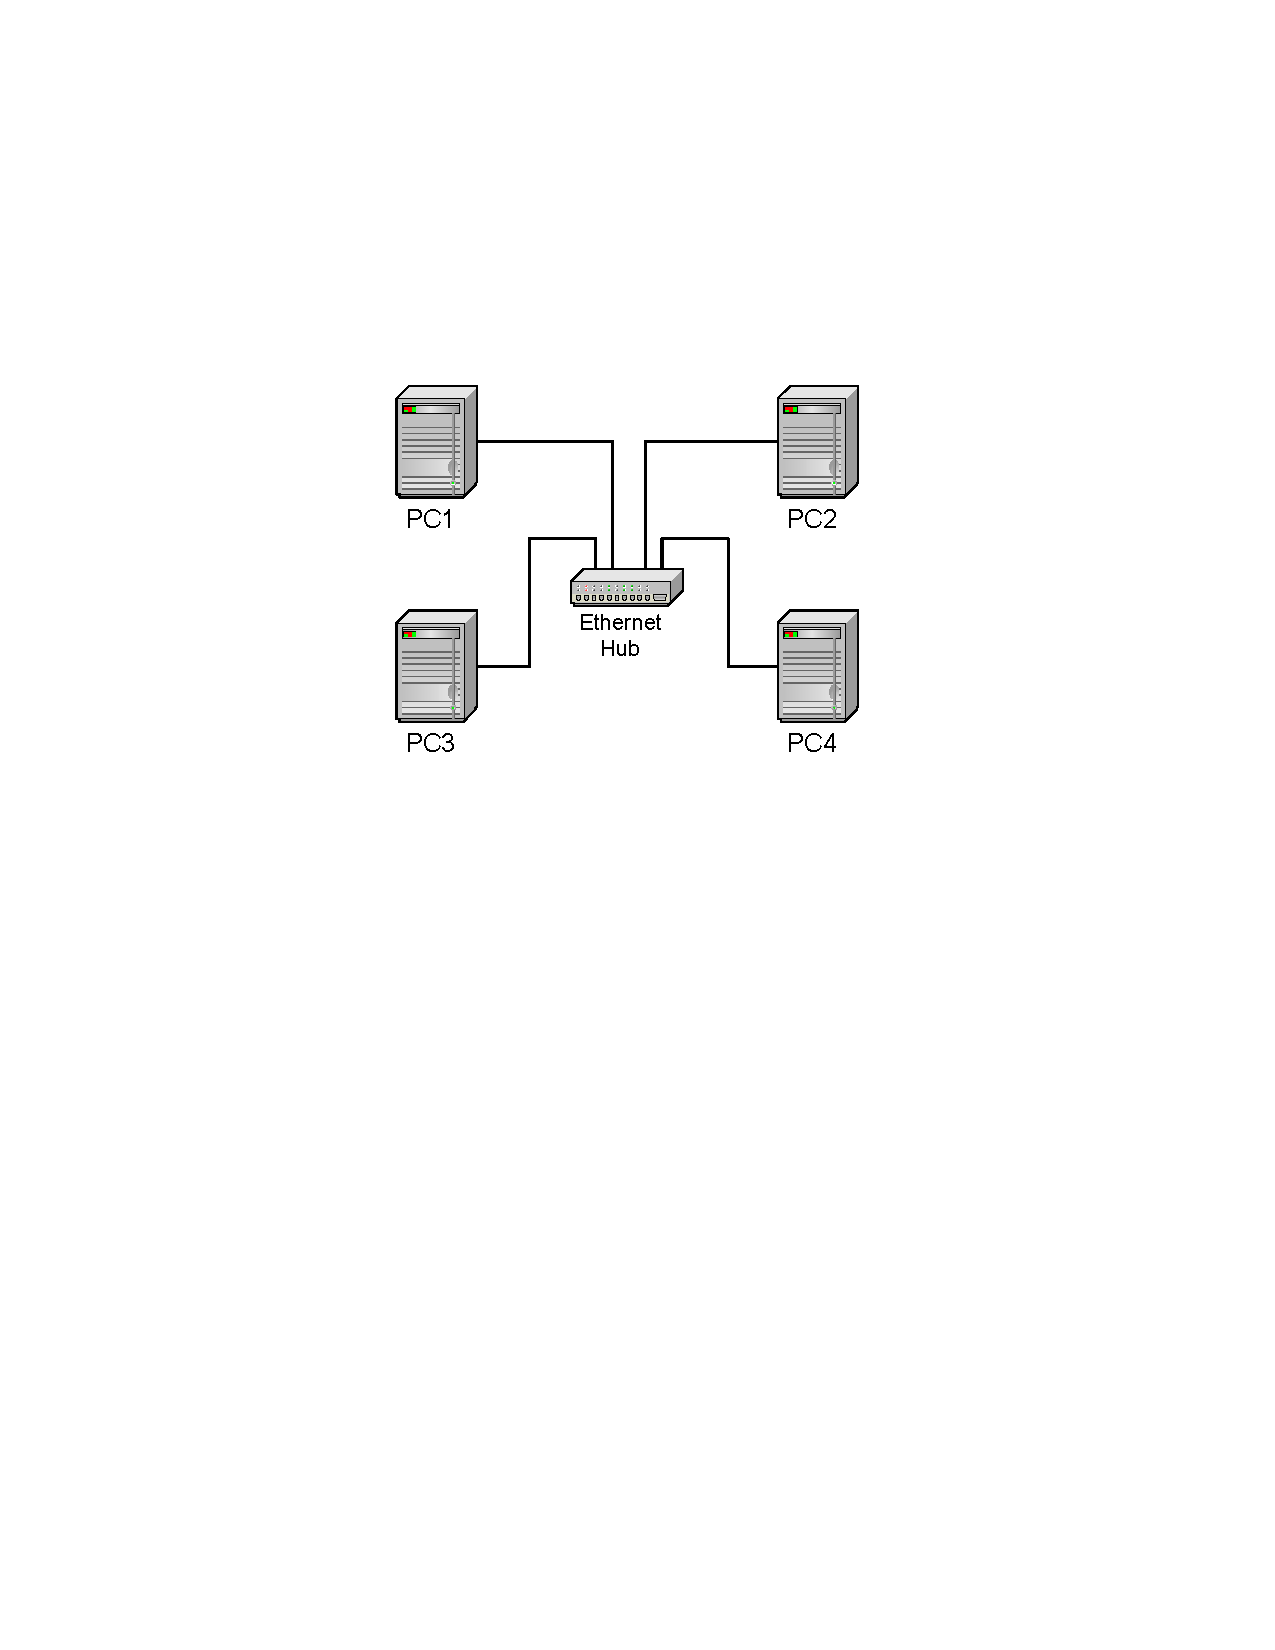
\includegraphics{graphics/lab1-network.pdf}	
	\caption{Network configuration for Lab 1.}
	\label{fig:lab1-network}
\end{figure}

\begin{itemize}
	\item All four Linux PCs are connected to a single Ethernet segment via a single hub as shown in Figure \ref{fig:lab1-network}.
	\item IP addresses for the Linux PCs are configured as in Table \ref{tab:lab1-ip-addresses}
		\begin{table}[ht]
			\centering
			\begin{tabular}{| c | c | c |}	
				\hline
				\textbf{Linux PC} & \textbf{IP Addresses of Ethernet Interface \iface{eth0}}  \\ \hline
				PC1 & 10.0.1.11/24 \\ 
				PC2 & 10.0.1.12/24 \\
				PC3 & 10.0.1.13/24 \\
				PC3 & 10.0.1.14/24 \\ \hline
			\end{tabular}
			\caption{IPv4 addresses for Lab 1}
			\label{tab:lab1-ip-addresses}
		\end{table}
	\item The notation 10.0.1.11/24 means that the IP address is 10.0.1.11 and the network prefix is 24 bits long. A network prefix of 24 bits corresponds to a netmask set to 255.255.255.0. With this netmask, all hosts are on the 10.0.1.0/24 network.
\end{itemize}


\subsubsection*{Mapping of the patch panel ports to the PC interfaces}
\begin{enumerate}
	\item Use the mapping in Table \ref{tab:lab1-patch-panel} to figure out which interface of which PC is which port on the patch panel. Connect the PC's to the hub using Ethernet cables.
		\begin{table}[ht]
			\centering
			\begin{tabular}{| c | c | c |}	
				\hline
				\textbf{Linux PC} & \textbf{Interface} & \textbf{Patch panel port}  \\ \hline
				PC1 & \iface{eth0} & 1 \\ 
				PC1 & \iface{eth1} & 2 \\ 
				PC2 & \iface{eth0} & 3 \\ 
				PC2 & \iface{eth1} & 4 \\ 
				PC3 & \iface{eth0} & 5 \\ 
				PC3 & \iface{eth1} & 6 \\ 
				PC4 & \iface{eth0} & 7 \\ 
				PC4 & \iface{eth1} & 8 \\ \hline
			\end{tabular}
			\caption{IP addresses for Lab 1}
			\label{tab:lab1-patch-panel}
		\end{table}
	\item Configure \iface{eth0} for each of the PCs. e.g. for PC1 use the following command.
		\begin{cmdblock}
	PC1% ifconfig eth0 10.0.1.11 netmask 255.255.255.0 broadcast 10.0.1.255 up
		\end{cmdblock}
		As an alternative, you can use th \cmd{ip} command:
		\begin{cmdblock}
	PC1% ip addr add 10.0.1.11/24 dev eth0
	PC1% ip link set dev eth0 up
		\end{cmdblock}
	\item Test connectivity by using \cmd{ping}, e.g.
		\begin{cmdblock}
	PC1% ping -c 5 10.0.1.11
		\end{cmdblock}
	\end{enumerate}

\newpage
\subsection{Locating Configuration Files in Linux}

Linux has numerous configuration files which set the environment variables of the operating system. For example, if you want to set up your Linux PC as an IP router, you merely need to change a single line in one of the configuration files. Studying configuration files also provides a way of learning what network configuration options are available to you.

\remark If you are unable to revert some of the changes you made, try rebooting the PC's as they will be reverted to their original settings.

\remark Configuration files are fundamentally different across different versions of Unix-like operating system (e.g., AIX, Solaris, Linux, FreeBSD). Sometimes the structure of configuration files changes between releases of the same Unix version. For example, the configuration files of different Linux distributions, such as, Ubuntu, Fedora, OpenSuSE at and Slackware, are quite different. Furthermore, the configuration files between different versions of the same Linux distribution can have significant differences.

The file \path{/etc/network/interfaces} contains settings on how the interfaces should be configured when starting the network service on Debian-based Linux distributions. You will notice that there is not much in this file as our lab PCs are preconfigured NOT to bring up their interfaces. You can read the man page to find out more on this file. It will not be used in the remainder of this course.

\begin{cmdblock}
	> man interfaces
\end{cmdblock}

You will not find much in \path{sysctl.conf} either: check out the \cmd{sysctl} tool and briefly browse \path{/proc/sys/net}. You will see that there are several parameters that allow you to tweak the behavior of the linux network stack.

\begin{cmdblock}
	> ls /proc/sys/net
	> man sysctl
\end{cmdblock}

The \path{/etc/hosts} files contains a mapping of hostnames to IP addresses.

\begin{cmdblock}
	> less /etc/hosts
\end{cmdblock}

\subsubsection*{Exercise 5. Network configuration files}
\begin{questions}
	\q{5.1}{Which file(s) must be edited to change the name of a Linux PC (e.g. from PC1 to machine1)?}
	\q{5.2}{Which file(s) include information that determines whether a Linux PC performs IP forwarding?}
\end{questions}

\newpage
\subsection{Using Ping}

One of the most basic, but also most effective tools to debug IP networks is the \cmd{ping} command. The ping command tests whether another host or router on the Internet is reachable. The \cmd{ping} command sends an ICMP Echo Request datagram to an interface, and expects an ICMP Echo Reply datagram in return.

Note:
\begin{itemize}
	\item On Linux systems, \cmd{ping} continues to send packets until you interrupt the command with the \cmd{Ctrl-c} keys.
	\item When using \cmd{ping} on the Linux PCs, we recommend to always send at least two ICMP Echo Request packets. We have observed that in some occasions, the first ICMP Echo Request may be dropped at the receiver.
\end{itemize}

\subsubsection*{Exercise 6. Issuing ping commands}

\begin{enumerate}
	\item From PC1, send 5 ping messages (using the -c option) to PC2. Save the output. 
		\begin{cmdblock}
	PC1% ping -c 5 10.0.1.12
		\end{cmdblock}
	\item On PC2, issue a ping to the IP address of PC1. Also, issue a \cmd{ping} command to the \iface{loopback} interface, \cmd{127.0.0.1}. Limit the number of pings to 5. Save the output.
\end{enumerate}

\begin{questions}
	\q{6.1}{Include the output you saved in the exercise.}
	\q{6.2}{Explain the difference between pinging the local Ethernet interface and the \iface{loopback} interface. Specifically, on PC1, what is the difference between typing \cmd{ping 10.0.1.11} and \cmd{ping 127.0.0.1}? (This is a conceptual question on the role of the \iface{loopback} interface. The response to the ping command does not provide you with the answer to this question.) Hint: Try using \cmd{tcpdump} or Wireshark, which are explained in the next section to verify your answer. Hint: Is this handled by software (the linux routing stack), hardware (the network card, hubs, switches, routers) or both?}
	\q{6.3}{Find a host connected to the Internet. Send ping messages to a number of web servers on the Internet and collect statistics on the maximum round-trip delay of the ICMP Echo Request/Echo Reply. Try to find a host with a very long round-trip time. To avoid overloading the destination, do not send more than 10 ping packets to any destination machine. Save the output data and include it in your lab report.}
\end{questions}

\newpage
\subsection{Basics of \cmd{tcpdump}}

\cmd{tcpdump} allows you to capture traffic on a network and display the packet headers of the captured traffic. \cmd{tcpdump} can be used to identify network problems or to monitor network activities.

\subsubsection*{Exercise 7-A. Simple \cmd{tcpdump} exercise}

Use \cmd{tcpdump} to observe the network traffic that is generated by issuing \cmd{ping} commands.
\begin{framed}
	If you use the \cmd{tee} or \cmd{tail} commands to simultaneously view and save the output from \cmd{tcpdump}, you need to use the \cmd{-l} option of \cmd{tcpdump}. For example:
	\begin{cmdblock}
	> tcpdump -n -l > filename & tail -f filename
	> tcpdump -n -l | tee filename
	\end{cmdblock}
	\emph{Note: It may be necessary to hit \cmd{Ctrl-c} to terminate the \cmd{tcpdump} session. In some situations, it may be best to simply redirect the output of \cmd{tcpdump} straight to a file (e.g., \cmd{tcpdump \textgreater filename}) and view it afterwards with the \cmd{less} command or a text editor.}
\end{framed}

\begin{enumerate}
	\item Switch to PC1. Start \cmd{tcpdump} so that it monitors all packets that contain the IP address of PC2, by typing
		\begin{cmdblock}
	PC1% tcpdump -n host 10.0.1.12
		\end{cmdblock}
	\item Open a new window and execute
		\begin{cmdblock}
	PC1% ping -c 1 10.0.1.12
		\end{cmdblock}
	\item Observe the output of \cmd{tcpdump}. Save the output to a file.
\end{enumerate}

\begin{questions}
	\q{7.A}{Include the saved output in your lab report. Explain the meaning of each field in the captured data.}
\end{questions}

\subsubsection*{Exercise 7-B. Another \cmd{tcpdump} traffic capture}
\begin{enumerate}
	\item On PC1, start capturing packets using the \cmd{tcpdump -n} command.
	\item Issue a ping to the non-existing IP address 111.111.111.111:
		\begin{cmdblock}
	PC1% ping -c 1 111.111.111.111
		\end{cmdblock}
	\item Issue a ping to the broadcast address 10.0.1.255 using the command:
		\begin{cmdblock}
	PC1% ping -c 2 -b 10.0.1.255
		\end{cmdblock}
		When sending pings to the broadcast address is not working, check out the \path{/proc/sys/net/ipv4/} directory for possible broadcast-related settings. Try enabling/disabling them if necessary (see the previous paragraph).
		\boxinfo{Explain what you did, what happened and why in the lab report. Simply stating that broadcast pings didn't work is not a correct answer.}
	\item Save the outputs of \cmd{ping} and \cmd{tcpdump} to a file.
\end{enumerate}

\begin{questions}
	\q{7.B}{Include the saved output in your lab report and interpret the results. How many of the Linux PCs responded to the broadcast ping? Why is this?}
\end{questions}

\newpage
\subsection{Basics of wireshark}

Wireshark is a network protocol analyzer with a graphical user interface. Using Wireshark, you can interactively capture and examine network traffic, view summaries and get detailed information for each packet.

\subsubsection*{Exercise 8. Running wireshark}

This exercise walks you through the steps of capturing and saving network traffic with Wireshark. The exercise is conducted on PC1.

\begin{figure}[ht]
	\centering
	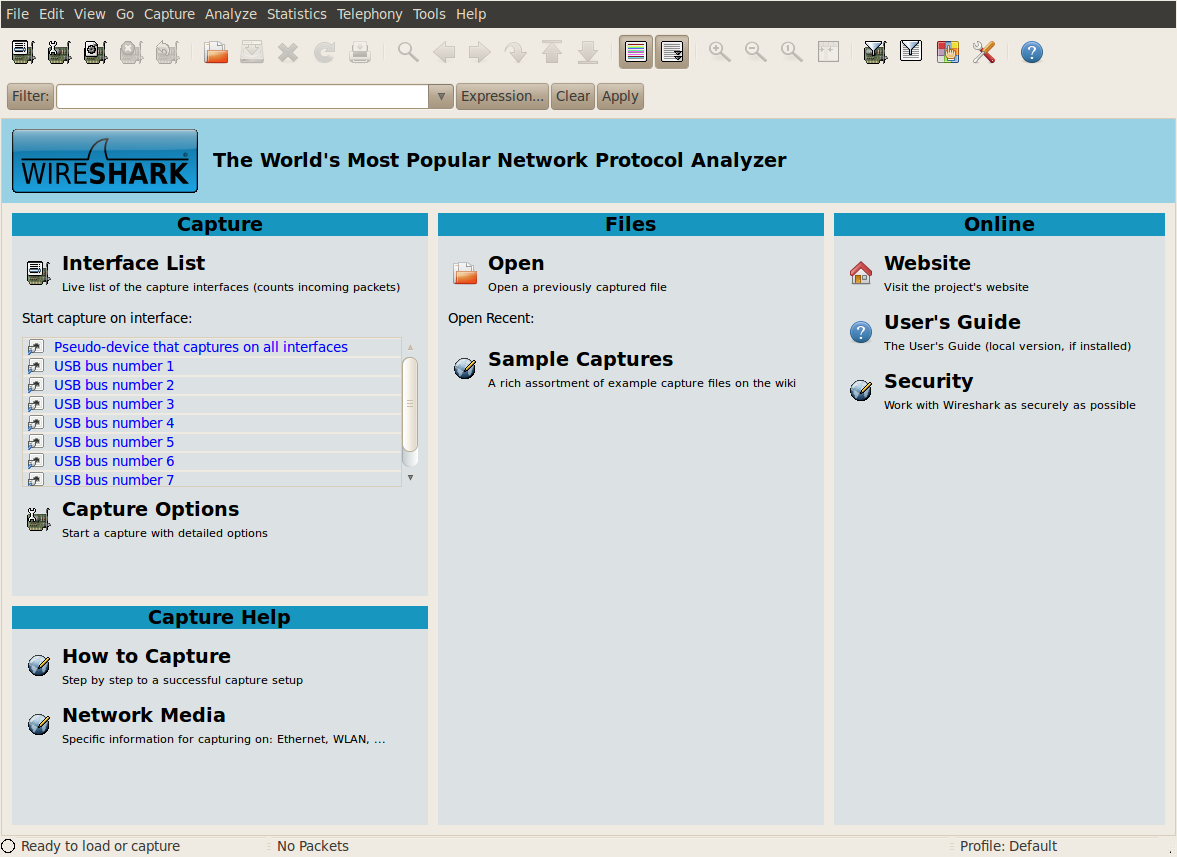
\includegraphics[width=\linewidth]{graphics/wireshark-main-updated.png}	
	\caption{Wireshark Main Window.}
	\label{fig:lab1-wireshark-main}
\end{figure}

\begin{enumerate}
	\item Starting Wireshark: On PC1, start Wireshark by typing 
		\begin{cmdblock}
	PC1% wireshark
		\end{cmdblock}
		This displays the Wireshark main window on your desktop as shown in Figure \ref{fig:lab1-wireshark-main}.
		\boxwarning{\textbf{Do not forget to start Wireshark with root permissions using \cmd{sudo} if you are not root already.}}
	\item Selecting the capture options: Use the instructions in Figure \ref{fig:lab1-capture-options} to set the options of Wireshark in preparation for capturing traffic. Use the same options in other labs, whenever Wireshark is started.
		\par
		\begin{minipage}{\linewidth}
			\begin{framed}
				\centering
				\textbf{Selecting capture preferences in Wireshark}
				\begin{enumerate}
					\item From the main window, select ``Capture:Start''.
					\item This displays the following ``Capture Preferences'' window:\par
						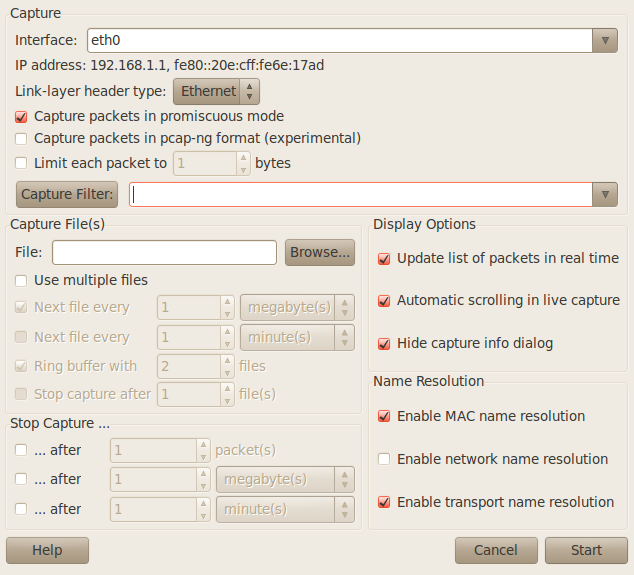
\includegraphics[width=\linewidth]{graphics/capture-options-updated.png}
						\begin{itemize}
							\item Select \iface{eth0} in ``Interface''.
							\item Select ``Capture packets in promiscuous mode''.
							\item Select ``Update list of packets in real time''.
							\item Select ``Automatic scrolling in live capture''.
							\item Unselect ``Enable MAC name resolution''.
							\item Unselect ``Enable network name resolution''.
							\item Unselect ``Enable transport name resolution''.
						\end{itemize}
				\end{enumerate}
			\end{framed}
			\captionof{figure}{General capture settings for Wireshark}
			\label{fig:lab1-capture-options}
		\end{minipage}

	\item Starting the traffic capture: Start the packet capture by clicking ``OK'' in the ``Capture Preferences'' window.

	\item Generating traffic: In a separate window on PC1, execute a \cmd{ping} command to PC3.
		\begin{cmdblock}
	PC1% ping -c 2 10.0.1.13
		\end{cmdblock}
		Observe the output in Wireshark's main window.
		Click and highlight a captured packet in the Wireshark window, and view the headers of the captured traffic.

	\item Stopping the traffic capture: Click ``Stop'' in the window ``Ethernet Capture''.

	\item Saving captured traffic: Save the results of the captured traffic as a plain text file. Use the instructions in Figure \ref{fig:lab1-print-options} in order to configure the print options..\par
		\begin{minipage}{\linewidth}
			\begin{framed}
				\centering
				\textbf{Selecting print options for saving captured traffic to plain text files}
				\begin{enumerate}
					\item From the main window, select ``File:Print''.
					\item This displays the following ``Printer oprions'' window:\par
					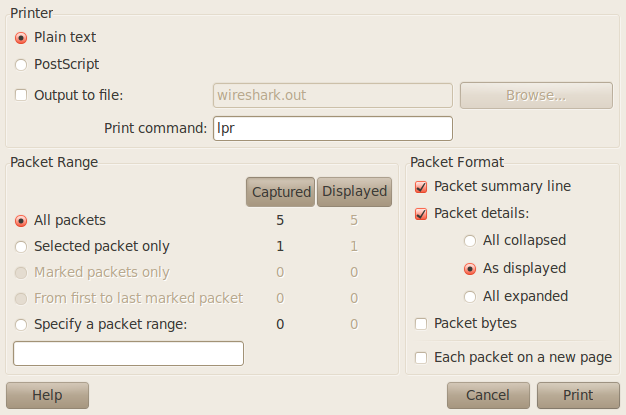
\includegraphics[width=\linewidth]{graphics/wireshark-print-updated.png}
					\begin{itemize}
						\item Select the format ``PlainText''.
						\item Select the ``File'' checkbox and type the filename in the field next to the ``File'' button.
						\item Select ``Print summary'' if you want to save only some high level information on each packet. Print summary is usually sufficient.
						\item Select ``Print detail'' and ``Expand all levels'' if you want to save all details of all packets at all levels.
						\item Click the ``OK'' button to complete the save operation.
					\end{itemize}
				\end{enumerate}
			\end{framed}
			\captionof{figure}{Selecting print options.}
			\label{fig:lab1-print-options}
		\end{minipage}\hspace*{\fill}
			\boxinfo{If you select ``Save'' in the ``File'' menu, the captured data is saved in the format of a libpcap file. This format can be interpreted by both \cmd{tcpdump} and Wireshark. Measurements saved in libpcap format can be analyzed at a later time. However, libpcap files are not plain text files and are not useful for preparing your report.}
			\boxinfo{In general, unless asked to do otherwise, always select the ``Print summary'' option when you include saved data in the lab report. This will help keep the length of the lab report reasonably small. If detailed information is required you will be asked to save ``details'' of the captured traffic. In this case, select the ``Print detail'' option.}
			\boxwarning{\textbf{Always include binary libpcap traces with your report, in addition to printed summaries or details that you use in the report to prove your answer is correct.}}
\end{enumerate}

\begin{questions}
	\q{8}{Include the file with the captured data in your lab report. Save the details of the captured traffic using the ``Print Detail'' option in the ``Print'' Window. Describe the differences between the files saved by \cmd{tcpdump} (in Part 7) and by Wireshark (in this part).}
\end{questions}

\setcounter {chapter} {1}
%%!TEX root = labo.tex

\chapter{Single-Segment IP Networks}

What you will learn in this lab:
\begin{itemize}
	\item How to capture and filter network traffic
	\item How to configure a network interface for IP networking
	\item How to access IP statistics and settings with the netstat command
	\item How ARP works
	\item How hackers snoop passwords from the network
\end{itemize}

\newpage
\setsession{prelab2}
\section{Prelab 2}\label{sec:prelab2}
%!TEX root = labo.tex

\subsubsection*{New commands}
Read the manual pages of the following commands at \url{http://manpages.ubuntu.com/} for the operating system version ``\osversion'':
\begin{itemize}
	\item arp
	\item ifconfig
	\item netstat
	\item tcpdump
\end{itemize}

\subsubsection*{IP Addresses}
Read the article ``Understanding IP Addressing: Everything You Ever Wanted To Know'' by Chuck Semeria, at \url{http://holdenweb.com/static/docs/3comip.pdf}

\subsubsection*{Wireshark capture and display filters}
Go to the Wireshark website and read about capture filters and display filters for Wireshark:
\begin{itemize} 
	\item \url{http://wiki.wireshark.org/CaptureFilters}
	\item \url{http://www.wireshark.org/docs/wsug_html_chunked/ChWorkBuildDisplayFilterSection.html}.
\end{itemize}

\newpage
\subsection*{Prelab Questions}

\begin{questions}
	\q{1}{Write the syntax for an \cmd{ifconfig} command that sets the IP address of the interface \iface{eth0} to 128.143.2.3/16 with broadcast address 128.143.255.255.}
	\q{2}{Write the syntax of a \cmd{tcpdump} command that captures packets containing IP datagrams with source or destination IP address equal to 10.0.1.12.}
	\q{3}{Write the syntax of a \cmd{tcpdump} command that captures packets containing ICMP messages with source or destination IP address equal to 10.0.1.12.}
	\q{4}{Write the syntax of a \cmd{tcpdump} command that captures packets containing IP datagrams between two hosts with IP addresses 10.0.1.11 and 10.0.1.12, both on interface \iface{eth1}.}
	\q{5}{Write a \cmd{tcpdump} filter expression that captures packets containing TCP segments with source or destination IP address equal to 10.0.1.12.}
	\q{6}{Write a \cmd{tcpdump} filter expression that, in addition to the constraints in Question 5, only captures packets using port number 23.}
	\q{7}{Write the syntax for a \cmd{wireshark} command with capture filter so that all IP datagrams with source or destination IP address equal to 10.0.1.12 are recorded.}
	\q{8}{Write the syntax for a Wireshark display filter that shows IP datagrams with destination IP address equal to 10.0.1.50 and frame sizes greater than 400 bytes.}
	\q{9}{Write the syntax for a Wireshark display filter that shows packets containing ICMP messages with source or destination IP address equal to 10.0.1.12 and frame numbers between 15 and 30.}
	\q{10}{Write the syntax for a Wireshark display filter that shows packets containing TCP segments with source or destination IP address equal to 10.0.1.12 and using port number 23.}
	\q{11}{Write a Wireshark capture filter expression for Question 10.}
\end{questions}


\newpage
\setsession{lab2}
\section{Lab 2}\label{sec:lab2}

In Lab 2 you become acquainted with IP configuration issues on a single Ethernet segment. The lab also exposes you to advanced use of \cmd{tcpdump} and Wireshark.

\begin{figure}[h!t]
	\centering
	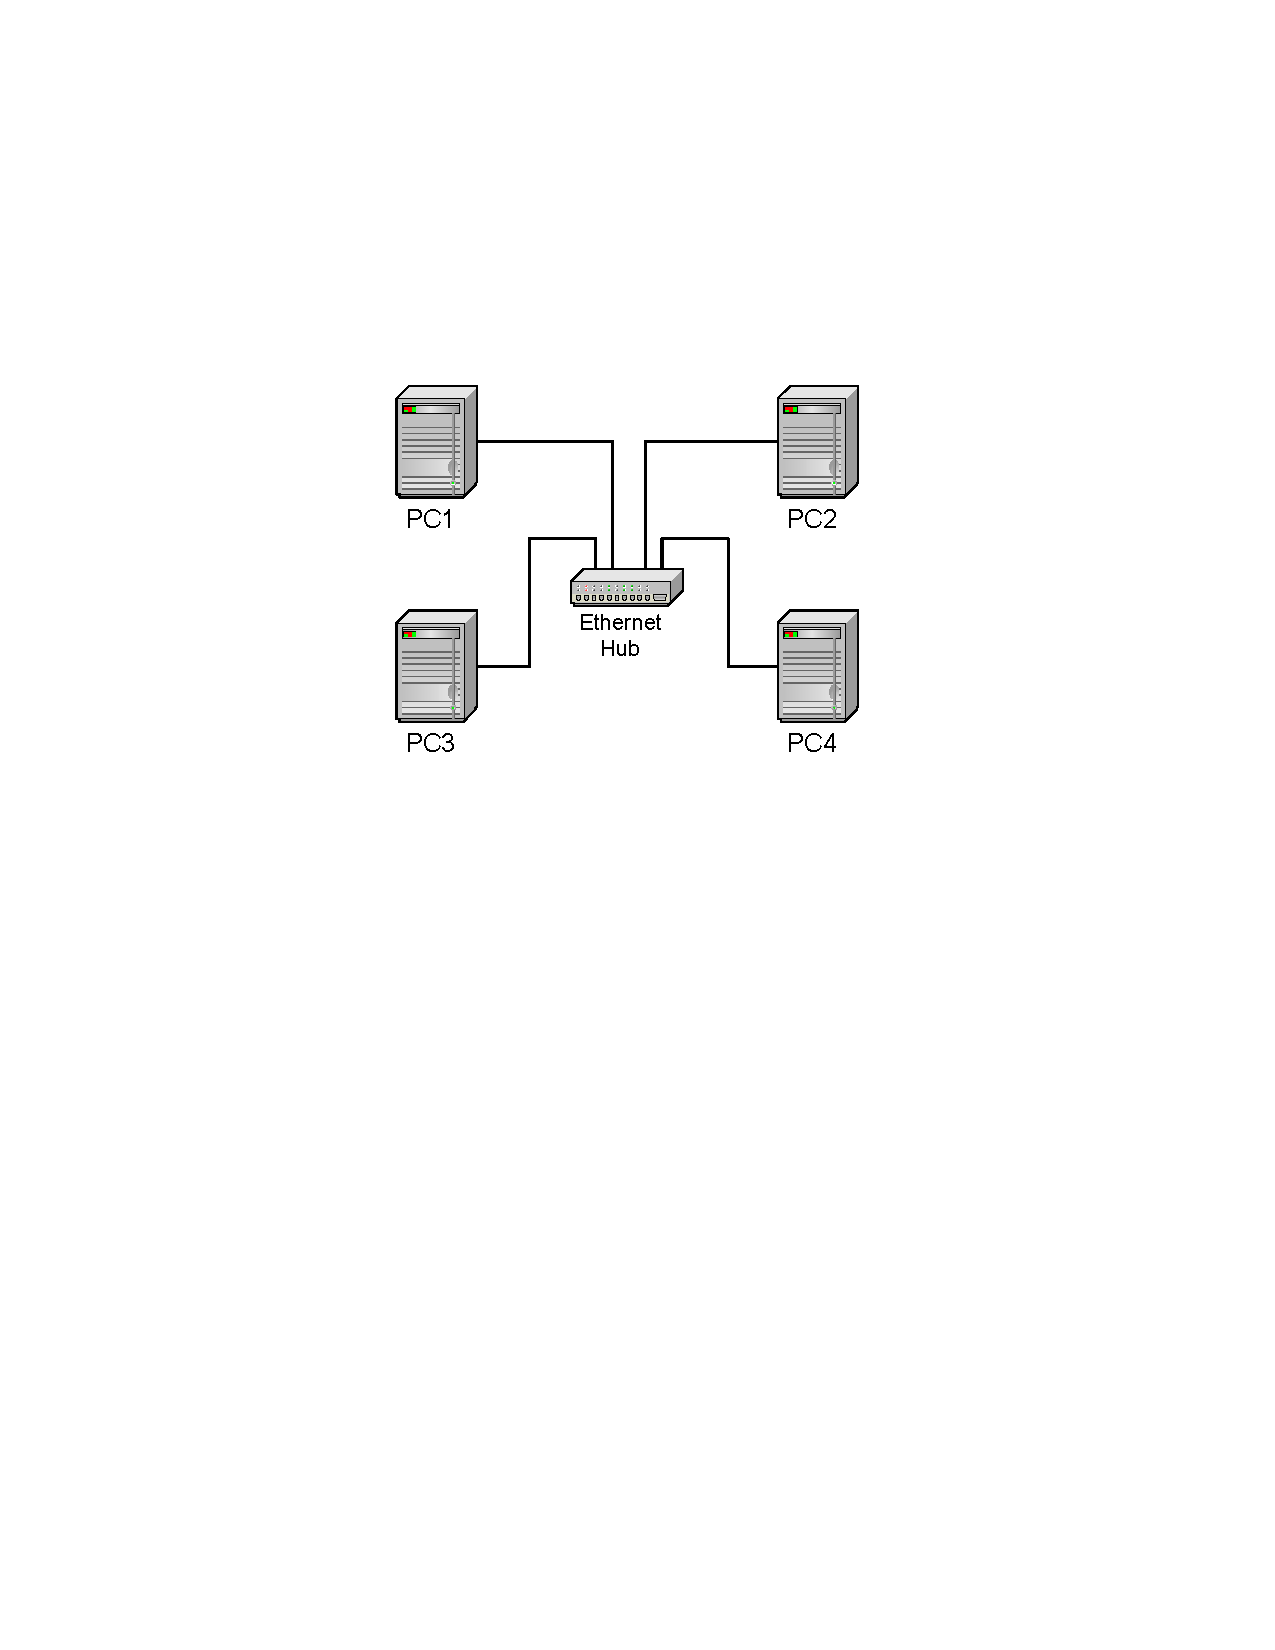
\includegraphics{graphics/lab1-network.pdf}	
	\caption{Network configuration for Lab 2.}
	\label{fig:lab2-network}
\end{figure}

The setup for this lab is identical as in Lab 1. All Linux PCs are connected to the same Ethernet segment by an Ethernet hub as shown in Figure \ref{fig:lab2-network}.
The IP addresses for the Linux PCs are configured as shown in Table \ref{tab:lab2-ip-addresses} below. Configure \iface{eth0} for each of the PCs. e.g. for PC1 use the following command.

\begin{cmdblock}
	PC1% ifconfig eth0 10.0.1.11 netmask 255.255.255.0 broadcast 10.0.255 up
\end{cmdblock}
As an alternative, you can use th \cmd{ip} command:
\begin{cmdblock}
	PC1% ip addr add 10.0.1.11/24 dev eth0
	PC1% ip link set dev eth0 up
\end{cmdblock}

\begin{table}[h!t]
	\centering
	\begin{tabular}{| c | c | c |}	
		\hline
		\textbf{Linux PC} & \textbf{IP Addresses of Ethernet Interface eth0}  \\ \hline
		PC1 & 10.0.1.11/24 \\ 
		PC2 & 10.0.1.12/24 \\
		PC3 & 10.0.1.13/24 \\
		PC3 & 10.0.1.14/24 \\ \hline
		\end{tabular}
	\caption{IPv4 addresses for Lab 2}
	\label{tab:lab2-ip-addresses}
\end{table}

\newpage
\subsection{Using filters in tcpdump}

In the first part of the lab, you explore \cmd{tcpdump} in more detail. In particular, you learn how to write filter expressions so that \cmd{tcpdump} monitors only selected traffic flows on the network. See \ref{sec:prelab2} for more details on the use of filters in \cmd{tcpdump}.

\subsubsection*{Exercise 1. Writing filter expressions for tcpdump}

In this exercise, you explore the use of simple filter expressions with the \cmd{tcpdump} command. Save the output for your lab report.

\begin{enumerate}
	\item On PC1, execute a \cmd{tcpdump} command with a filter that prints all packets with PC2 as source or destination. This command is the answer to Question 2 from the Prelab. Save the output of this \cmd{tcpdump} session to a file using the tee or tail commands discussed in Lab 1.\hspace*{\fill}
		\boxinfo{As in Lab 1, always use the \cmd{-n} option (i.e. \cmd{tcpdump -n}) to avoid that \cmd{tcpdump} tries to resolve hostnames.}
	\item In another terminal, issue a ping command to PC2 by typing \cmd{ping -c 5 10.0.1.12} on PC1 and observe the output. Recall that the ping command to a host triggers the transmission of an ICMP Echo Request. The destination host responds with an ICMP Echo Reply message.
	\item Repeat steps 1 - 2 above. In addition to the existing filter, set the filter so that only ICMP messages are captured. This command is the answer to Question 3 from the Prelab.
\end{enumerate}

\boxwarning{\textbf{Make sure to include the saved data in your lab report as they are part of your evaluation!}}

\newpage
\subsection{Using filters in Wireshark}

In this part of the lab, you experiment with filter expressions using the \cmd{wireshark} command. Recall that Wireshark has two types of filters: capture filters and display filters.

\boxinfo{There are several command line options that can be assigned when starting the \cmd{wireshark} command:\hspace*{\fill}
}
\begin{itemize}
	\item{\textbf{Capture Filters:}} A capture filter specifies the traffic to be captured by the Wireshark tool. A capture filter expression can be specified from the command line using the \cmd{-f} option or using the Wireshark GUI, under the ``Capture:Start'' menu. The syntax for specifying the filter expression is the same syntax as used by \cmd{tcpdump}.
	\item{\textbf{Display Filters:}} By default, Wireshark displays all captured packets. With a display filter, just those packets, which meet the requirements of the filter, are displayed. The display filter cannot be set from the command line. It must be entered in the ``Filter'' window at the bottom of the GUI. The syntax for setting the display filter is different from the syntax for setting a capture filter.
	\item{\textbf{Setting an interface:}} When you run Wireshark on a host with multiple network interfaces, you may specify the interface with the \cmd{-i} argument. For example, to start Wireshark to capture traffic on interface \iface{eth1}, type
		\begin{cmdblock}
	wireshark -i eth1
		\end{cmdblock}		
		If you do not specify an interface, the default is \iface{eth0}. Alternatively, you can change the interface using the Wireshark GUI, under the ``Capture:Start'' menu.
\end{itemize}

\subsubsection*{Exercise 2-A. Setting capture filters in Wireshark}
This exercise is a review of the traffic capture capabilities of Wireshark. As a new feature, you are introduced to the notion of capture filters.

\begin{enumerate}
	\item Start Wireshark on PC1 and set the same capture preferences as in Lab 1 and as shown again in Figure \ref{fig:lab2-capture-options} for your convenience. You should always set these same preferences for all your experiments.\par
		\begin{minipage}{\linewidth}
			\begin{framed}
				\centering
				\textbf{Selecting capture preferences in wireshark} \\
				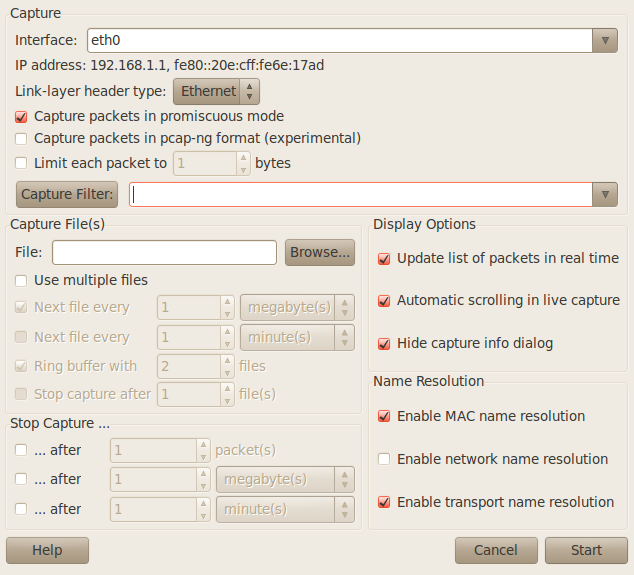
\includegraphics[width=\linewidth]{graphics/capture-options-updated.png}
				\begin{itemize}
					\item Select \iface{eth0} in ``Interface''.
					\item Select ``Capture packets in promiscuous mode''.
					\item Select ``Update list of packets in real time''.
					\item Select ``Automatic scrolling in live capture''.
					\item Unselect ``Enable MAC name resolution''.
					\item Unselect ``Enable network name resolution''.
					\item Unselect ``Enable transport name resolution''.
				\end{itemize}
			\end{framed}
			\captionof{figure}{General capture settings for Wireshark}
			\label{fig:lab2-capture-options}
		\end{minipage}
	\item Setting a capture filter: In the window ``Capture Preferences'', set a filter so that all packets that contain the IP address of PC2 are recorded. The filter is set in the ``Filter'' box under ``Capture Preferences'' (see Figure \ref{fig:lab2-capture-options}). The required filter expression is the answer to Question 7 from the Prelab.
	\item Start the capture by clicking ``OK'' in the ``Capture Preferences'' window.
	\item In another terminal window of PC1, issue a \cmd{ping} command to PC2
		\begin{cmdblock}
	PC1% ping -c 2 10.0.1.12
		\end{cmdblock}
	\item Stop the capture process of Wireshark.
	\item Save the results of the capture. This is done by selecting ``Print'' in the ``File'' menu as described in Lab 1. (As instructed in Lab 1, unless asked to save the details of captured frames, selecting the summary option is usually sufficient.)
\end{enumerate}

\boxwarning{\textbf{Make sure to include the saved data in your lab report as they are part of your evaluation!}}

\subsubsection*{Exercise 2-B. Working with display filters}

Next you set display filters, which allow you to select a subset of the captured data for display in the main window of Wireshark.

\begin{enumerate}
	\item In the Wireshark main window on PC1 from Exercise 2-A, set the display options as listed below. You can find the display options in the ``Capture Options'' window (select "Start" in the "Capture" menu)(see Figure \ref{fig:lab2-capture-options}):\par
		\begin{itemize}
			\item Select ``Update list of packets in real time''.
			\item Select ``Automatic Scrolling in live capture''.
			\item Unselect ``Enable MAC name resolution''.
			\item Unselect ``Enable network name resolution''.
			\item Unselect ``Enable transport name resolution''.
		\end{itemize}
	\item Setting a display filter: Type the desired display filter in the field next to the ``Filter'' box, which is located at the bottom of the Wireshark main window, as shown in Figure \ref{fig:lab2-display-filter}. Click the ``Reset'' button next to the ``Filter'' box to clear any existing filter:\par
		\begin{minipage}{\linewidth}
			\centering
			
\includegraphics[width=\linewidth]{graphics/display-filter-updated.png}
			\captionof{figure}{Filter box for setting display filters.}
			\label{fig:lab2-display-filter}
		\end{minipage}
		Enter a display filter so that all IP datagrams with destination IP address 10.0.1.12 are shown. Refer to Question 8 from the Prelab.
	\item Observe the changes in the display panel of Wireshark. Only packets with 10.0.1.12 in the IP destination address field are now being displayed.
	\item Save the displayed data, by selecting ``File:Print''. Note that the ``Print'' command only saves packets that are currently being displayed. If a display filter is used, the saved data is limited to the packets that match the display filter.
	\item Repeat the above exercise with a display filter that lists only IP datagrams with source IP address equal to 10.0.1.12. Save the results.		
\end{enumerate}

\boxwarning{\textbf{Make sure to include the saved data in your lab report as they are part of your evaluation!}}

\subsubsection{Exercise 2-C. More complex capture and display filters}

In this exercise, you learn how to use more sophisticated filters to restrict the packets being captured and displayed.

\begin{enumerate}
	\item Start Wireshark on PC1 and start to capture traffic using the same settings as in Exercise 2-A. Do not set any capture or display filters!
	\item From a new terminal on PC1, execute the \cmd{ping} command for PC2 
		\begin{cmdblock}
	PC1% ping -c 5 10.0.1.12
		\end{cmdblock}
	\item At the same time, start a Telnet session from PC1 to PC2 in another terminal by typing
		\begin{cmdblock}
	PC1% telnet 10.0.1.12
		\end{cmdblock}
		and log in as \textit{telecomlabo}. After you logged in successfully to PC2, logout with the command \cmd{exit}.
	\item Stop the traffic capture of wireshark.
	\item Apply a set of display filters to the captured traffic and save the output to a text file. Select the option ``Print summary'' in the ``Print'' window.
		\begin{itemize}
			\item Display packets that contain ICMP messages with the IP address of PC2 either in the IP destination address or IP source address. Refer to Question 9 from the Prelab. Save the output.
			\item Display packets that contain TCP traffic with the IP address of PC2 either in the IP destination address or IP source address. Refer to Question 10 from the Prelab. Save the output.
			\item Display packets that, in addition to the constraints in the previous filter expression, use the port number 23. Refer to Question 10 from the Prelab. Save the output.
		\end{itemize}
\end{enumerate}

\boxwarning{\textbf{Make sure to include the saved data in your lab report as they are part of your evaluation!}}

\newpage
\subsection{ARP - Address Resolution Protocol}

This part of the lab explores the operation of the Address Resolution Protocol (ARP) which resolves a MAC address for a given IP address. The lab exercises use the Linux command \cmd{arp} for displaying and manipulating the contents of the ARP cache. The ARP cache is a table that holds entries of the form \textless IP address, MAC address\textgreater.

\boxinfo{The most common uses of the \cmd{arp} command are as follows:
	\begin{description}
		\item[\texttt{arp -a}]\hfill \\
			Displays the content of the ARP cache.
		\item[\texttt{arp -d \textless IPAddress\textgreater}] \hfill \\
			Deletes the entry with IP address IPAddress.
		\item[\texttt{arp -s \textless IPAddress\textgreater \textless MAC\_Address\textgreater}] \hfill \\
			Adds a static entry to the ARP cache which is never overwritten by network events. The MAC address is entered as a 6 hexadecimal bytes separated by colons.\\
			Example: \texttt{arp -s 00:02:2D:0D:68:C1}
	\end{description}
}

\boxinfo{\textbf{Time-outs in the ARP cache:}\hfill \\
	The entries in an ARP cache have a limited lifetime. Entries are deleted unless they are refreshed. The typical lifetime of an ARP entry is 2 minutes, but much longer lifetimes (up to 20 minutes) have been observed. You may want to verify when your Linux system does remove ARP entries automatically after a certain amount of time.}

\boxinfo{\textbf{Refreshing the ARP cache:}\hfill \\
	In Linux, you will observe that occasionally, a host sends out ARP requests to interfaces that are already in the ARP cache. Example: Suppose that a host with IP address 10.0.1.12 has an ARP cache entry: ``\textless10.0.1.11\textgreater is-at \textless00:02:83:39:2C:42\textgreater''. Then, this host occasionally sends a unicast ARP Request to MAC address 00:02:83:39:2C:42 of the form ``Who has 10.0.1.11? Tell 10.0.1.12'' to verify that the IP address 10.0.1.11 is still present before deleting the entry from the ARP cache.}

\subsubsection*{Exercise 3-A. A simple experiment with ARP}
\begin{enumerate}
	\item On PC1, view the ARP cache with \cmd{arp -a} and delete all entries with the \cmd{-d}  option.
	\item Start Wireshark on PC1 with a capture filter set to the IP address of PC2.
	\item Issue a ping command from PC1 to PC2:
		\begin{cmdblock}
	PC1% ping -c 2 10.0.1.12
		\end{cmdblock}
	Observe the ARP packets in the Wireshark window. Explore the MAC addresses in the Ethernet headers of the captured packets. Direct your attention to the following fields:
		\begin{itemize}
			\item The destination MAC address of the ARP Request packets.
			\item The Type field in the Ethernet headers of ARP packets and ICMP messages.
		\end{itemize}
	\item View the ARP cache again with the command \cmd{arp -a}. Note that ARP cache entries get refreshed/ deleted fairly quickly (approx. 2 minutes).
	\item Save the results of Wireshark to a pcap dump file.
\end{enumerate}

Use the saved data to answer to the following questions:

\begin{questions}
	\q{3.A.1}{What is the destination MAC address of an ARP Request packet?}
	\q{3.A.2}{What are the different values of the Type field in the Ethernet headers that you observed?}
	\q{3.A.3}{Use the captured data to discuss the process in which ARP acquires the MAC address for IP address 10.0.1.12.}
\end{questions}
	
\subsubsection*{Exercise 3-B. Matching IP addresses and MAC addresses}
Identify the MAC addresses of all interfaces connected to the network, and enter them in Table \ref{tab:lab2-ip-to-mac}. You can obtain the MAC addresses from the ARP cache of each PC. You can fill up the ARP cache at a host, by issuing a ping command from that host to every other host on the network. Alternatively, you can obtain the MAC addresses from the output of the \cmd{ifconfig -a} command explained in Part 5.

\begin{table}[h!t]
	\centering
	\begin{tabular}{| c | c | c |}	
		\hline
		\textbf{Linux PC} & \textbf{IP Address of eth0} & \textbf{MAC Address of eth0} \\ \hline
		PC1 & 10.0.1.11/24 & \\ 
		PC2 & 10.0.1.12/24 & \\
		PC3 & 10.0.1.13/24 & \\
		PC3 & 10.0.1.14/24 & \\ \hline
	\end{tabular}
	\caption{ IP and MAC addresses.}
	\label{tab:lab2-ip-to-mac}
\end{table}

\begin{questions}
	\q{3.B.1}{Include the completed Table \ref{tab:lab2-ip-to-mac} in your lab report.}
\end{questions}

\subsubsection*{Exercise 3-C. ARP requests for a non-existing address}

Observe what happens when an ARP Request is issued for an IP address that does not exist.

\begin{enumerate}
	\item On PC1, start wireshark with a capture filter set to capture packets that contain the IP address of PC1:
		\begin{cmdblock}
	PC1% wireshark -f 'host 10.0.1.11'
		\end{cmdblock}
	\item Establish a Telnet session from PC1 to 10.0.1.10 (Note that this address does not exist on this network)
		\begin{cmdblock}
	PC1% telnet 10.0.1.10
		\end{cmdblock}
		Observe the time interval and the frequency with which PC1 transmits ARP Request packets. Repeat the experiment a number of times to discover the pattern.
	\item Save the captured output.
\end{enumerate}

\begin{questions}
	\q{3.C.1}{Using the saved output, describe the time interval between each ARP Request packet issued by PC1. Describe the method used by ARP to determine the time between retransmissions of an unsuccessful ARP Request. Include relevant data to support your answer.}
	\q{3.C.2}{Why are ARP Request packets not transmitted (i.e. not encapsulated) as IP packets? Explain your answer.}
\end{questions}

\newpage
\subsection{The netstat command}

The Linux command \cmd{netstat} displays information on the network configuration and activity of a Linux system, including network connections, routing tables, interface statistics, masquerade connections, and multicast memberships. The following exercise explores how to use the \cmd{netstat} command to extract different types of information about the network configuration of a host.

\boxinfo{The most common uses of the \cmd{netstat} command are as follows:
	\begin{description}
		\item[\texttt{netstat -i}]\hfill \\
			Displays a table with statistics of the currently configured network interfaces.
		\item[\texttt{netstat -rn}] \hfill \\
			Displays the kernel routing table. The \cmd{-n} option forces \cmd{netstat} to print the IP addresses. Without this option, \cmd{netstat} attempts to display the hostnames.
		\item[\texttt{netstat -an; netstat -tan; netstat -uan}] \hfill \\
			 Displays the active network connections. The \cmd{-a} option displays all active network connections, the \cmd{-ta} option displays only information on TCP connections, and the \cmd{-ua} option displays only information on UDP traffic. Omitting the \cmd{-n} options prints hostnames and names of servers, instead of IP addresses and ports numbers.
		\item[\texttt{netstat -s}] \hfill \\
			Displays summary statistics for each protocol that is currently running on the host.
	\end{description}
}


\subsubsection*{Exercise 4. Basic usage of the netstat command}
On PC1, try the different variations of the \cmd{netstat} command listed above and save the output to a file.

\begin{enumerate}
	\item Display information on the network interfaces by typing
		\begin{cmdblock}
	PC1% netstat -in
		\end{cmdblock}
	\item Display the content of the IP routing table by typing
		\begin{cmdblock}
	PC1% netstat -rn
		\end{cmdblock}
	\item Display information on TCP and UDP ports that are currently in use by typing
		\begin{cmdblock}
	PC1% netstat -a
		\end{cmdblock}
	\item Display the statistics of various networking protocols by typing
		\begin{cmdblock}
	PC1% netstat -s
		\end{cmdblock}
\end{enumerate}

\boxinfo{The values of the statistics displayed by some of the \cmd{netstat} commands are reset each time a host is rebooted.}


\begin{questions}
	\q{4.1}{Attach the saved output to your report. Using the saved output, answer the following questions.}
	\q{4.1.a}{What are the network interfaces of PC1 and what are the MTU (Maximum Transmission Unit) values of the interfaces?}
	\q{4.1.b}{How many IP datagrams, ICMP messages, UDP datagrams, and TCP segments has PC1 transmitted and received since it was last rebooted?}
	\q{4.2}{Explain the role of interface lo, the loopback interface. In the output of "netstat -in", why are the values of RX-OK (packets received) and TX-OK (packets transmitted) different for interface "eth0" but identical for interface lo?}
\end{questions}

\newpage	
\subsection{Configuring IP interfaces in Linux}

The \cmd{ifconfig} command is used to configure parameters of network interfaces on a Linux system, such as enabling and disabling of interfaces and setting the IP address. The \cmd{ifconfig} command is usually run when a system boots up. In this case, the parameters of the commands are read from a file. Once the Linux system is running, the \cmd{ifconfig} command can be used to modify the network configuration parameters.

\boxinfo{The most common uses of the \cmd{ifconfig} command to query the status of network interfaces are as follows:
	\begin{description}
		\item[\texttt{ifconfig}]\hfill \\
			Displays the configuration parameters of all active interfaces.
		\item[\texttt{ifconfig -a}] \hfill \\
			Displays the configuration parameters of all network interfaces, including the inactive interfaces.
		\item[\texttt{ifconfig \textless interface>\textgreater}] \hfill \\
			Displays the configuration parameters of a single interface. For example, \cmd{ifconfig eth0} displays information on interface \iface{eth0}.
	\end{description}
}

\boxinfo{There are numerous options for configuring a network interface with \cmd{ifconfig}. The following example shows how to enable and disable an interface and how to change the IP configuration.
	\begin{description}
		\item[\texttt{ifconfig eth0 down}]\hfill \\
			Disables the eth0 interface. No traffic is sent or received on a disabled interface.
		\item[\texttt{ifconfig eth0 up}]\hfill \\
			Enables the eth0 interface.
		\item[\texttt{ifconfig eth0 10.0.1.8 netmask 255.255.255.0 broadcast 10.0.1.255}]\hfill \\
			Assigns interface \iface{eth0} the IP address 10.0.1.8/24 and a broadcast address of 10.0.1.255. The interface should be disabled before a new IP address is assigned, and should be enabled after the IP address has been modified.
		\item[\texttt{ifconfig eth0 down 10.0.1.8 netmask 255.255.255.0 broadcast 10.0.1.255 up}]\hfill \\
			Performs all three commands above in sequence. Interface \iface{eth0} is disabled, an IP address and a broadcast address are assigned, and the interface is enabled.
		\item[\texttt{ifconfig eth0 mtu 500}]\hfill \\
			Sets the MTU of interface \iface{eth0} to 500 bytes.
	\end{description}
}

\subsubsection*{Exercise 5. Changing the IP address of an interface}

Use the \cmd{ifconfig} command to modify the IP address of the \iface{eth0} interface of PC4.
\begin{enumerate}
	\item On PC4, run \cmd{ifconfig -a} and save the output.
	\item Change the IP address of interface \iface{eth0} of PC4 to 10.0.1.11/24.
	\item Run \cmd{ifconfig -a} again and save the output.
\end{enumerate}

\begin{questions}
	\q{5.1}{Attach the saved files to your report and explain the fields of the \cmd{ifconfig} output.}
\end{questions}
	
\newpage
\subsection{Duplicate IP addresses}
In this part of the lab, you observe what happens when two hosts have identical IP addresses.

\subsubsection*{Exercise 6. Duplicate IP addresses}
\begin{enumerate}
	\item After completing Exercise 5, the IP addresses of the Ethernet interfaces on the four PCs are as shown in the Table \ref{tab:lab2-ip-addresses-part-6}. Note that PC1 and P4 are assigned the same IP address.

		\begin{table}[h!t]
			\centering
			\begin{tabular}{| c | c | c |}	
				\hline
				\textbf{Linux PC} & \textbf{IP Addresses of Ethernet Interface eth0}  \\ \hline
				PC1 & 10.0.1.11/24 \\ 
				PC2 & 10.0.1.12/24 \\
				PC3 & 10.0.1.13/24 \\
				PC3 & 10.0.1.11/24 \\ \hline
			\end{tabular}
			\caption{IP addresses for Part 6}
			\label{tab:lab2-ip-addresses-part-6}
		\end{table}
	\item Delete all entries in the ARP cache on all PCs.
	\item Run wireshark on PC3 and capture the network traffic to and from the duplicate IP address 10.0.1.11
	\item From PC3, start a Telnet session to the duplicate IP address, 10.0.1.11, by typing
		\begin{cmdblock}
	PC3% telnet 10.0.1.11
		\end{cmdblock}
		and log in as \textit{telecomlabo} user, using the \textit{mvkbj1n} password.
	\item Once you have logged in, determine the name of the host to which you are connected. The name of the host can be determined in several ways: (1) issue the command \cmd{hostname}, (2) inspect the ARP cache on PC3, or (3) interpret the captured Wireshark packets.
	\item Stop the traffic capture in Wireshark.
	\item Save all ARP packets and the first few TCP packets captured by Wireshark. Also save the ARP cache of PC3 using the \cmd{arp -a} command.
	\item When you are done with the exercise, reset the IP address of PC4 to its original value as given in Table \ref{tab:lab2-ip-addresses}.
\end{enumerate}

\begin{questions}
	\q{6.1}{Explain why the Telnet session was established to one of the hosts with the duplicate address and not the other. Explain why the Telnet session was established at all, and did not result in an error message. Use the ARP cache and the captured packets to support your explanation.}
\end{questions}

\newpage
\subsection{Changing netmasks}

In this part of the lab you test the effects of changing the netmask of a network configuration. In the table below, two hosts (PC2 and PC4) have been assigned different network prefixes.

\boxwarning{If you are having difficulties understanding the concept of netmasks, try using a subnet calculator tool. You can find one at  \url{http://subnet-calculator.com} or most operating systems have native tools or widgets that can do the same.}

\subsubsection*{Exercise 7.}

\begin{enumerate}
	\item Setup the interfaces of the hosts as shown in Table \ref{tab:lab2-ip-addresses-part-7}. Note that the netmasks of the hosts are different.
		\begin{table}[h!t]
			\centering
			\begin{tabular}{| c | c | c |}	
				\hline
				\textbf{Linux PC} & \textbf{IP Addresses of eth0} & \textbf{Netmask} \\ \hline
				PC1 & 10.0.1.100/24 & 255.255.255.0 \\ 
				PC2 & 10.0.1.101/28 & 255.255.255.240 \\
				PC3 & 10.0.1.120/24 & 255.255.255.0 \\
				PC3 & 10.0.1.121/28 & 255.255.255.240 \\ \hline
			\end{tabular}
			\caption{IP addresses for Part 7}
			\label{tab:lab2-ip-addresses-part-7}
		\end{table}
	\item Run Wireshark on PC1 and capture the packets for the following ping commands
		\begin{enumerate}[label=\alph*.]
			\item From PC1 to PC3:
				\begin{cmdblock}
	PC1% ping -c 1 10.0.1.120
				\end{cmdblock}
			\item From PC1 to PC2:
				\begin{cmdblock}
	PC1% ping -c 1 10.0.1.101
				\end{cmdblock}
			\item From PC1 to PC4:
				\begin{cmdblock}
	PC1% ping -c 1 10.0.1.121
				\end{cmdblock}
			\item From PC4 to PC1:
				\begin{cmdblock}
	PC1% ping -c 1 10.0.1.100
				\end{cmdblock}
			\item From PC2 to PC4:
				\begin{cmdblock}
	PC1% ping -c 1 10.0.1.121
				\end{cmdblock}
			\item From PC2 to PC3:
				\begin{cmdblock}
	PC1% ping -c 1 10.0.1.120
				\end{cmdblock}
		\end{enumerate}
	\item Save the Wireshark output, and save the output of the ping commands. Note that not all of the above scenarios are successful. Save all output, including any error messages.
	\item When you are done with the exercise, reset the interfaces to their original values as given in Table \ref{tab:lab2-ip-addresses}.
\end{enumerate}

\begin{questions}
	\q{7.1}{Use your output data and ping results to explain what happened in each of the \cmd{ping} commands. Which ping operations were successful and which were unsuccessful? Why?
		\boxwarning{\textbf{You get credits for answering the 'why?' question, not for stating the obvious.}}}
\end{questions}

\newpage
\subsection{Static mapping of IP addresses and hostnames}

Since it is easier to memorize names than IP addresses, there are mechanisms to associate a symbolic name, called \emph{hostname}, with an IP address. On the Internet, the resolution between hostnames and IP addresses is generally done by the Domain Name System (DNS), which will not be discussed in this course. This experiment illustrates another, simpler method to map IP addresses and domain names using the host file \path{/etc/hosts}.

Before DNS became available, the \path{/etc/hosts} file was the only method to resolve hostnames in the Internet. All hosts on the Internet had to occasionally synchronize with the content of other \path{/etc/hosts} files.

\subsubsection*{Exercise 8. Associating names with IP addresses}

In this exercise, you manipulate the static mapping of hostnames and IP addresses using the \path{/etc/hosts} file.
\begin{enumerate}
	\item On PC1, inspect the content of file \path{/etc/hosts} with a text editor.
	\item On PC1, issue a \cmd{ping} command to PC2
		\begin{cmdblock}
	PC1% ping 10.0.1.12
		\end{cmdblock}
	\item Repeat Step 2, but use symbolic names instead of IP addresses (e.g., PC2 instead of 10.0.1.12). You should see that the symbolic name is unreachable at this point.
	\item On PC1, edit the file \path{/etc/hosts} and associate hostnames with the IP addresses and save the changes. Use the names PC1, PC2, etc., as used throughout this lab to refer to the PCs.
	\item Repeat Step 3. You should now be able to ping directly using the hostnames ``PC2'', ``PC3'', ``PC4'', as in:
		\begin{cmdblock}
	PC1% ping PC2
	PC1% ping PC3
	PC1% ping PC4
		\end{cmdblock}
	\item Reset the \path{/etc/hosts} file to its original state. That is, remove the changes you have made in this exercise, and save the file.
\end{enumerate}

\begin{questions}
	\q{8.1}{Explain why a static mapping of names and IP addresses is impractical when the number of hosts is large.}
	\q{8.2}{What will be the result of the hostname resolution when multiple IP addresses are associated with the same hostname in the \path{/etc/hosts} file?}
\end{questions}

\newpage
\subsection{Experiments with FTP and Telnet}

A severe security problem with the file transfer protocol (FTP) is that the login and password information are transmitted as plain text (not encrypted). Sometimes malicious users exploit this by snooping passwords on the network.

Here you learn how easy it is to crack passwords by snooping traffic from FTP and Telnet sessions.

\boxerror{\textbf{The use of applications that do not encrypt passwords, such as FTP and Telnet, is strongly discouraged. On the Internet, you should use protocols such as Secure Shell (SSH) tools for file transfers and remote login.}}

\subsubsection*{Exercise 9-A. Snoop Passwords from an FTP session}

Capture traffic from an FTP session between two hosts.

The ftp server installed on the lab PC's is vsftpd, which is not started by default. Use the following command to start it on PC2:

\begin{cmdblock}
	PC2% service vsftpd start
\end{cmdblock}

\begin{enumerate}
	\item On PC1, run the Wireshark command with capture filters set to capture traffic between PC1 and PC2. The capture filter is
		\begin{cmdblock}
	host 10.0.1.11 and host 10.0.1.12
		\end{cmdblock}
	\item On PC1, initiate a FTP session to PC2 by typing
		\begin{cmdblock}
	PC1% ftp 10.0.1.12
		\end{cmdblock}
	\item Log in as \textit{telecomlabo} user.
	\item Inspect the payload of packets with FTP payload that are sent from PC1 to PC2. FTP sessions use TCP connections for data transfer.
		\boxinfo{In Wireshark, there is a simple method to view the payload sent in a TCP connection. Simply select a packet that contains a TCP segment in the main window of Wireshark, and then click on ``Follow TCP Stream'' in the ``Tools'' menu of the Wireshark window. This will create a new window that displays only the payload of the selected TCP connection.}
	\item Save the details of the packets, i.e., select ``Print details'' in the ``Print'' window of Wireshark, which transmit the login name and password. As a hint, you can set the display filter in Wireshark to show only the desired packet(s). Refer to Question 9 from the Prelab.
\end{enumerate}

\begin{questions}
	\q{9.A.1}{Using the saved output, identify the port numbers of the FTP client and the FTP server.}
	\q{9.A.2}{Identify the login name and the password, shown in plain text in the payload of the packets that you captured.}
\end{questions}


\subsubsection*{Exercise 9-B. Snoop Passwords from a Telnet session}

Repeat the above exercise with the \cmd{telnet} command instead of ftp. On PC1, establish a Telnet session to PC2, and save the Wireshark output of packets used to transmit the login name and password.

\begin{questions}
	\q{9.B}{Does Telnet have the same security flaws as FTP? Support your answer using the saved output.}
\end{questions}

\subsubsection*{Exercise 9-C. Observing traffic from a Telnet session}

This exercise uses the Telnet session established in the previous exercise.
\begin{enumerate}
	\item Run Wireshark on PC1, and start to capture traffic. If the Wireshark window from the previous exercise is still open, make sure that Wireshark is capturing traffic.
	\item If the Telnet session from the previous exercise is still in place, skip to the next step. Otherwise, follow the steps from the previous exercise and log in from PC1 to PC2 with the \cmd{telnet} command.
	\item Once you are logged in, type a few characters. Observe the number of packets, captured by Wireshark, for each character typed. Observe that for each key you type, there are three packets transmitted. Determine why this occurs.
	\item Save the Wireshark output to a text file (using the ``Print Summary'' option).
\end{enumerate}

\begin{questions}
	\q{9.C}{Attach the saved output to your report. Explain why three packets are sent in a telnet session for each character typed on the terminal.}
\end{questions}

\setcounter {chapter} {2}
%%!TEX root = labo.tex

\chapter{Static Routing}

What you will learn in this lab:

\begin{itemize}
	\item How to turn a computer with multiple interfaces into a router
	\item How to set up static routing on Linux PC-routers and Cisco commercial routers
	\item How ICMP messages update routing table entries
	\item How Proxy ARP helps to connect different networks without reconfiguring the hosts
	\item How to work with different network prefixes
\end{itemize}

\newpage
\setsession{prelab3}
\section{Prelab 3}\label{sec:prelab3}
%!TEX root = labo.tex

\subsubsection*{Network Commands in Linux}
Read the manual pages of the following commands at \url{http://manpages.ubuntu.com/} for the operating system version ``\osversion'':
\begin{itemize}
	\item \cmd{route}
	\item \cmd{traceroute}
	\item \cmd{minicom}: This lab uses the \cmd{minicom} utility program to establish a serial connection between a Linux PC and a Cisco router.
\end{itemize}

\subsubsection*{{Proxy ARP}}
Go to the website of Cisco at \url{http://goo.gl/ixuktT} and read about Proxy ARP.

\subsubsection*{Cisco IOS}
The Cisco routers in the Lab are running a recent version of the Cisco Internet Operating System (IOS). Read about the IOS at \url{http://goo.gl/UD23vX}. Note that this is reference material that you can use. You are not expected to go through all of the manuals listed here!

\remark The most useful manuals for this course are the ``IP Application Services Configuration Guide'' and ``Cisco IOS IP Switching Configuration Guide''.

\newpage
\subsection*{Prelab Questions}

\begin{questions}
	\q{1}{What is the IOS command to change the MTU (maximum transmission unit) for an interface on a Cisco router?}
	\q{2}{How does a router determine whether a datagrams to particular host can be directly delivered through one of its interfaces?}
	\q{3}{Which systems generate ICMP Route Redirect messages? Routers, hosts, or both?}
	\q{4}{What is the default maximum TTL value used by traceroute when sending UDP datagrams?}
	\q{5}{Describe the role of a default gateway in a routing table?}
	\q{6}{What is the network prefix of IP address 192.110.50.3/24?}
	\q{7}{Explain the difference between an IP address and a network prefix.}
	\q{8}{An organization has been assigned the network number 140.25.0.0/16 and it needs to create networks that support up to 60 hosts on each IP network. What is the maximum number of networks that can be set up? Explain your answer.}
\end{questions}


\newpage
\setsession{lab3}
\section{Lab 3}\label{sec:lab3}

In this lab you work with four different network topologies. The topology for Parts 1-4 is shown in Figure \ref{fig:lab3-network1}. These parts address router configuration on a Linux PC and a Cisco Router. The topology for Part 5 is shown in Figure \ref{fig:lab3-network2}. This topology is used to study the role of ICMP route redirect message. For Part 6 we add one more router to the topology of Part 5 and examine the effect of routing loops as displayed in Figure \ref{fig:lab3-network3}. The topology for Part 7 is shown in Figure \ref{fig:lab3-network4}. There, you explore the relationship between network prefixes and IP forwarding.

%FIXME: subfigures in memoire...
%\begin{figure}
%	\centering
%	\subbottom[Part 1 - 4]{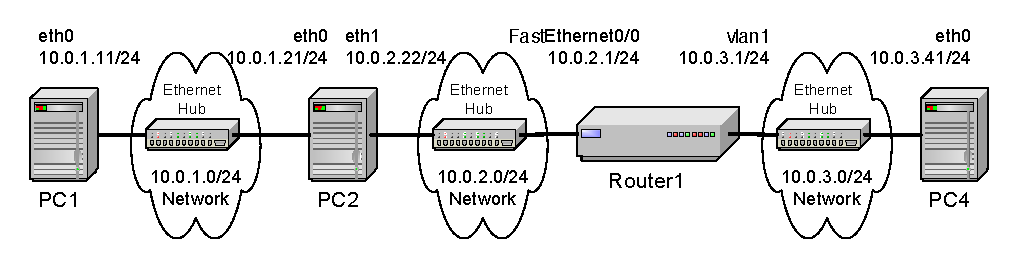
\includegraphics[width=0.4\linewidth]{graphics/lab3-network1-updated.pdf}}
%	\subbottom[Part 5]{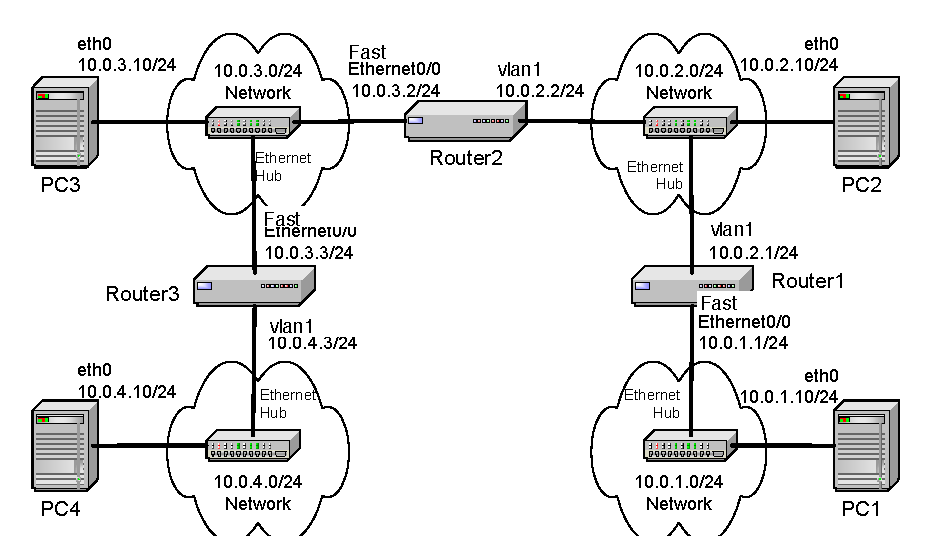
\includegraphics[width=0.4\linewidth]{graphics/lab3-network2-updated.pdf}}
%	\subbottom[Part 6]{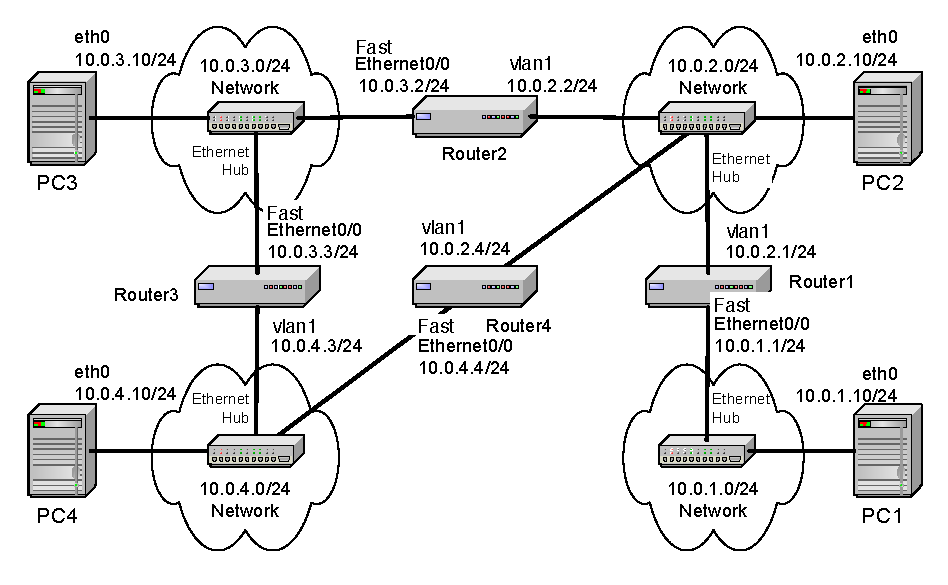
\includegraphics[width=0.4\linewidth]{graphics/lab3-network3-updated.pdf}}
%	\subbottom[Part 7]{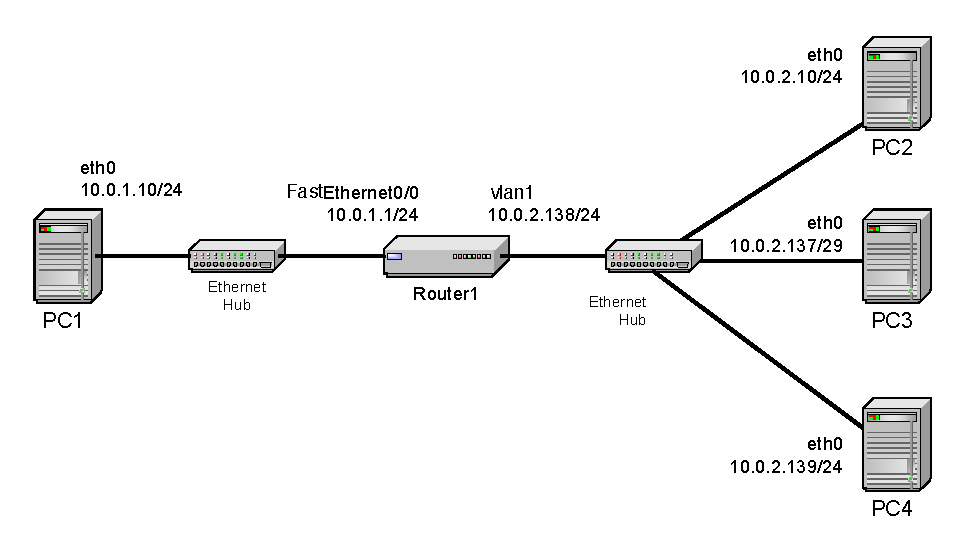
\includegraphics[width=0.4\linewidth]{graphics/lab3-network4-updated.pdf}}
%	\caption{Overview of the networks used in Lab \thechapter}
%  \label{fig:lab3-overview-networks}
%\end{figure}


\newpage
\subsection{Configuring a Linux PC as a Router}
Any Linux PC with at least two network interfaces can be set up as an IP router. Configuring a Linux PC as an IP router involves two steps: (1) modifying the configuration of Linux, so that IP forwarding is enabled and (2) configuring the routing table . Figure \ref{fig:lab3-network1} shows the network topology used in Parts 1 - 4 of this lab. PC1 and PC4 are used as hosts, and PC2 and Router1 are set up as IP routers. The PCs and the Cisco router are connected by three Ethernet hubs. In Lab 3, all routing table entries are manually configured, a procedure known as static routing.

\begin{figure}[h!t]
	\centering
	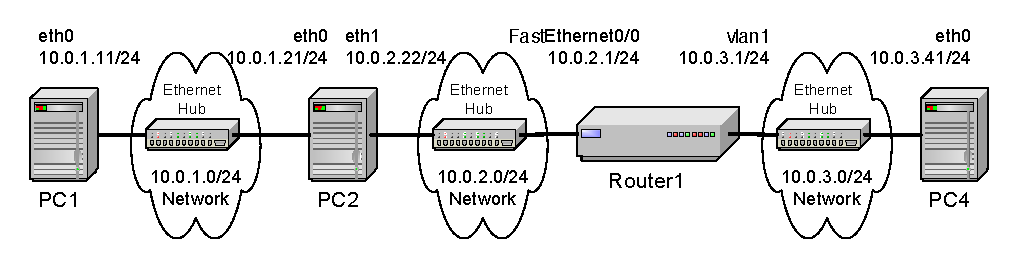
\includegraphics[width=\linewidth]{graphics/lab3-network1-updated.pdf}	
	\caption{Network configuration for Parts 1-4}
	\label{fig:lab3-network1}
\end{figure}

\begin{table}[h!t]
	\centering
	\begin{tabular}{| c | c | c |}	
		\hline
		\textbf{Linux PC} & \textbf{eth0} & \textbf{eth1} \\ \hline
		PC1 & 10.0.1.11/24 & Disabled \\ 
		PC2 & 10.0.1.21/24 & 10.0.2.22/24 \\
		PC3 & 10.0.3.41/24 & Disabled \\ \hline
		\textbf{Cisco Router} & \textbf{FastEthernet0/0} & \textbf{vlan1} \\ \hline
		Router1 & 10.0.2.1/24 & 10.0.3.1/24 \\ \hline
	\end{tabular}
	\caption{IP addresses for Parts 1-4}
	\label{tab:lab3-network1}
\end{table}

\subsubsection*{Exercise 1-A. Network setup}

\begin{enumerate}
	\item  Connect the Ethernet interfaces of the Linux PCs and the Cisco router as shown in Figure \ref{fig:lab3-network1}. Configure the IP addresses of the interfaces as given in Table \ref{tab:lab3-network1}.
	\item Start to capture traffic on PC1 with Wireshark.
	\item Issue a \cmd{ping} command from PC1 to PC2, Router1 and PC4. Save the output of each \cmd{ping} command.
		\begin{cmdblock}
PC1% ping -c 5 10.0.1.21 
PC1% ping -c 5 10.0.2.1 
PC1% ping -c 5 10.0.3.41
		\end{cmdblock}
	\item Save the captured wireshark output.
\end{enumerate}

Use the saved data to answer the following questions:

\begin{questions}
	\q{1.A.1}{What is the output on PC1 when the \cmd{ping} commands are issued?}
	\q{1.A.2}{Which packets, if any, are captured by Wireshark?}
	\q{1.A.3}{Do you observe any ARP or ICMP packets? If so, what do they indicate?}
	\q{1.A.4}{Which destinations are not reachable? Explain.}
\end{questions}
	
\subsubsection*{Exercise 1-b. Configuring a Linux PC as a router}

On a Linux system, IP forwarding is enabled when the file \path{/proc/sys/net/ipv4/ip_forward} contains a 1 and disabled when it contains a 0. Hence, enabling IP forwarding is done by writing a 1 in the file, with the command
\begin{cmdblock}
	PC1% echo "1" > /proc/sys/net/ipv4/ip_forward
\end{cmdblock}

The command echo writes the given argument, here, the string ``1'' to the standard output. Using the redirect operator (\textgreater ) and a file name, the output of the command is written to a file. IP forwarding is disabled with the command

\begin{cmdblock}
	PC1% echo "0" > /proc/sys/net/ipv4/ip_forward
\end{cmdblock}

The command has an immediate effect. However, changes are not permanent and are lost when the system is rebooted. Modifying the IP forwarding state permanently requires changes to the configuration file \path{/etc/sysctl.conf}. IP forwarding is enabled if the file contains a line \cmd{net.ipv4.ip\_forward = 1}, and IP forwarding is disabled when the line does not exist or the file contains the line \cmd{net.ipv4.ip\_forward = 0}. Changes to the configuration file \path{/etc/sysctl.conf} take effect the next time when Linux is rebooted.

Enable PC2 as an IP router using the command:

\begin{cmdblock}
	PC2% echo "1" > /proc/sys/net/ipv4/ip_forward
\end{cmdblock}

\subsubsection*{Exercise 1-c. Setting static routing table entries for a Linux PC}
Next, you must set up the routing tables of the Linux PCs. PC1 and PC4 are hosts, and PC2 is an IP router. The routing tables are configured so that they conform to the network topology shown in Figure \ref{fig:lab3-network1} and Table \ref{tab:lab3-network1}. The routes are configured manually, which is also referred to as static routing.

Configuring static routes in Linux is done with the command \cmd{route}, which has numerous options for viewing, adding, deleting or modifying routing entries. The various uses of the \cmd{route} command are summarized below.

\begin{itemize}
	\item Add a routing table entry for the network prefix identified by IP address netaddress and netmask mask. The next hop is identified by IP address gw\_address or by interface \iface{iface}.
		\begin{cmdblock}
	route add -net netaddress netmask mask gw gw_address 
	route add -net netaddress netmask mask dev iface
		\end{cmdblock}
	\item Add a host route entry for IP address hostaddress with next hop identified by IP address gw\_address or by interface \iface{iface}.
		\begin{cmdblock}
	route add -host hostaddress gw gw_address 
	route add -host hostaddress dev iface
		\end{cmdblock}
	\item Set the default route to IP address gw\_address.
		\begin{cmdblock}
	route add default gw gw_address
		\end{cmdblock}
	\item Delete an existing route from the routing table. It is not necessary to type all arguments. If enough arguments are provided so that it can be matched with an existing routing entry, the first entry that matches the given arguments is deleted.
		\begin{cmdblock}
	route del -net netaddress netmask mask gw gw_address 
	route del -host hostaddress gw gw_address
	route del default gw gw_address
		\end{cmdblock}
	\item Display the current routing table with extended fields. The command is identical to the \cmd{netstat -r} command.
		\begin{cmdblock}
	route -e 
	netstat -r
		\end{cmdblock}
	\item Display the routing table cache.
		\begin{cmdblock}
	route -C
		\end{cmdblock}
\end{itemize}

The command for adding a route for the network prefix 10.21.0.0/16 with next hop address 10.11.1.4 is
\begin{cmdblock}
	PC1% route add -net 10.21.0.0 netmask 255.255.0.0 gw 10.11.1.4
\end{cmdblock}

The command to add a host route to IP address 10.0.2.31 with the next hop set to 10.0.1.21 is
\begin{cmdblock}
	PC1% route add -host 10.0.2.31 gw 10.0.1.21
\end{cmdblock}

The command to add the IP address 10.0.4.4 as the default gateways is done with the command
\begin{cmdblock}
	PC1% route add default gw 10.0.4.4
\end{cmdblock}

The commands to delete the entries created with the above commands are
\begin{cmdblock}
	PC1% route del -net 10.21.0.0 netmask 255.255.0.0 PC1%route del -host 10.0.2.31
	PC1% route del default
\end{cmdblock}

There is no simple way to delete all entries in the routing table. One method to flush the routing table is to disable the interface and then enable the interface, as in
\begin{cmdblock}
	PC1% ifconfig eth0 down up
\end{cmdblock}

\boxinfo{The following commands are helpful to get information on routing and to find mistakes in the routing setup:
	\begin{description}
		\item[\texttt{ping IPaddress}] \hfill \\
			Tests if IPaddress can be reached. 
		\item[\texttt{traceroute IPaddress}] \hfill \\
			Displays the route to the interface IPaddress.
	\end{description}
}

When the commands are issued interactively in a Linux Shell, the added entries are valid until Linux is rebooted. To make static routes permanent on Debian-based Linux distributions, the routes need to be entered in the configuration file \path{/etc/network/interfaces} as post-up commands.

\begin{enumerate}
	\item  Configure the routing table entries of PC1 and PC4. You can either specify a default route or you insert separate routing entries for each remote network. For this exercise, add a route for each individual remote network. As a hint, here is the configuration information for PC4:
		\begin{cmdblock}
	PC4%route add -net 10.0.2.0 netmask 255.255.255.0 gw 10.0.3.1 
	PC4%route add -net 10.0.1.0 netmask 255.255.255.0 gw 10.0.3.1
		\end{cmdblock}
	\item Configure the routing table entries of the IP router PC2. (The correctness of the routing entries will be tested after Router1 has been setup.)
	\item Display the routing table of PC1, PC2, and PC4 with netstat -rn and save the output.
\end{enumerate}

\begin{questions}
	\q{1.C.1}{Include the saved output of the routing table. Explain the entries in the routing table and discuss the values of the fields for each entry.}
\end{questions}
	
\newpage
\subsection{Configuring a Cisco Router}

The setup of the Cisco router is more involved. The first step is to establish a physical connection to the router, so that configuration commands can be entered. There are different ways to connect to a Cisco router. In the Internet Lab, you will establish a serial connection to the router. This is done with a serial cable that connects the serial port of a Linux PC to the console port of a Cisco router. The next step is to run a terminal emulation program on the Linux PC. In the Internet Lab, you use the \cmd{minicom} software to access the router. Lastly, you have to type IOS (Internet Operating System) commands using the command line interface of IOS. The network setup for this part is as shown in Figure \ref{fig:lab3-network1} and Table \ref{tab:lab3-network1}.

\subsubsection*{Exercise 2-a. Accessing a Cisco router via the console port with Minicom}

Each lab is equipped with 4 cisco 1760 routers and each PC is connected through a serial cable to one of the routers, i.e., PC1 is connected to Router1, PC2 is connected to Router2, etc. You can use the \cmd{minicom} command to establish a remote terminal connection to the router. You will use Router1 and PC1 as the console.

Access the console port of Router1 from PC1 using \cmd{minicom} by typing:
\begin{cmdblock}
	PC1% minicom
\end{cmdblock}

If the connection is successful, you see a command prompt (User EXEC prompt) from Router1

\begin{cmdblock}
	Router1>
\end{cmdblock}

When you see this prompt, you can type Cisco IOS commands. If the prompt does not appear, then hit Enter key several times.

To terminate a \cmd{minicom} session, type \cmd{Ctrl-A}, then \cmd{Z} which will show a menu. Exit by typing \cmd{Q} and following the instructions.

\subsubsection{Exercise 2-b. Switching Cisco IOS command modes}

This exercise demonstrates how to log into a router and how to operate through the different Cisco IOS command modes. It is important to understand the different modes so you know where you are and what commands are accepted at any time.
\begin{enumerate}
	\item Start a \cmd{minicom} session on PC1 which is connected to Router1 with a serial cable.
	\item When PC1 is connected to the router, you see the prompt of the user EXEC mode (\cmd{Router\textgreater}). To see which commands are available in this mode, type a question mark (\cmd{?}):
		\begin{cmdblock}
	Router1> ?
		\end{cmdblock}
	\item To view and change system parameters of a Cisco router, you must enter the privileged EXEC mode, by typing:
		\begin{cmdblock}
	Router1> enable 
	Password : <enable secret> 
	Router1#
		\end{cmdblock}
		You need a password, the enable secret, to enter the privileged EXEC mode.
	\item To modify system wide configuration parameters, you must enter the global configuration mode. This mode is entered by typing:
		\begin{cmdblock}
	Router1# configure terminal
	Router1(config)#
		\end{cmdblock}
	\item To make changes to a network interface, enter the interface configuration mode, with the command:
		\begin{cmdblock}
	Router1(config)# interface FastEthernet0/0 
	Router1(config-if)#
		\end{cmdblock}
		The name of the interface is provided as an argument. Here, the network interface that is configured is \iface{FastEthernet0/0}.
	\item To return from the interface configuration to the global configuration mode, or from the global configuration mode to the privileged EXEC mode, use the exit command:
		\begin{cmdblock}
	Router1(config-if)# exit 
	Router1(config)# exit 
	Router1#
		\end{cmdblock}
		The exit command takes you one step up in the command hierarchy. To directly return to the privileged EXEC mode from any configuration mode, use the end command:
		\begin{cmdblock}
	Router1(config-if)# end Router1#
		\end{cmdblock}
	\item To return from the privileged EXEC mode to the user EXEC mode, type: 
		\begin{cmdblock}
	Router1# disable
	Router1>
		\end{cmdblock}
	\item To terminate the console session from the user EXEC mode, type: 
		\begin{cmdblock}
	Router1> logout
	Router1 con0 is now available Press RETURN to get started.
		\end{cmdblock}
		Or type \cmd{logout} or \cmd{exit} from the privileged EXEC mode: 
		\begin{cmdblock}
	Router1# exit
	Router1 con0 is now available Press RETURN to get started.
		\end{cmdblock}
\end{enumerate}

\subsubsection*{Exercise 2-c. Configuring IP interfaces on a Cisco router}

For this course we will be working with the Cisco 1760 Router, which is shown in Figure \ref{fig:cisco1760}.

\begin{figure}[h!t]
    \begin{center}  
      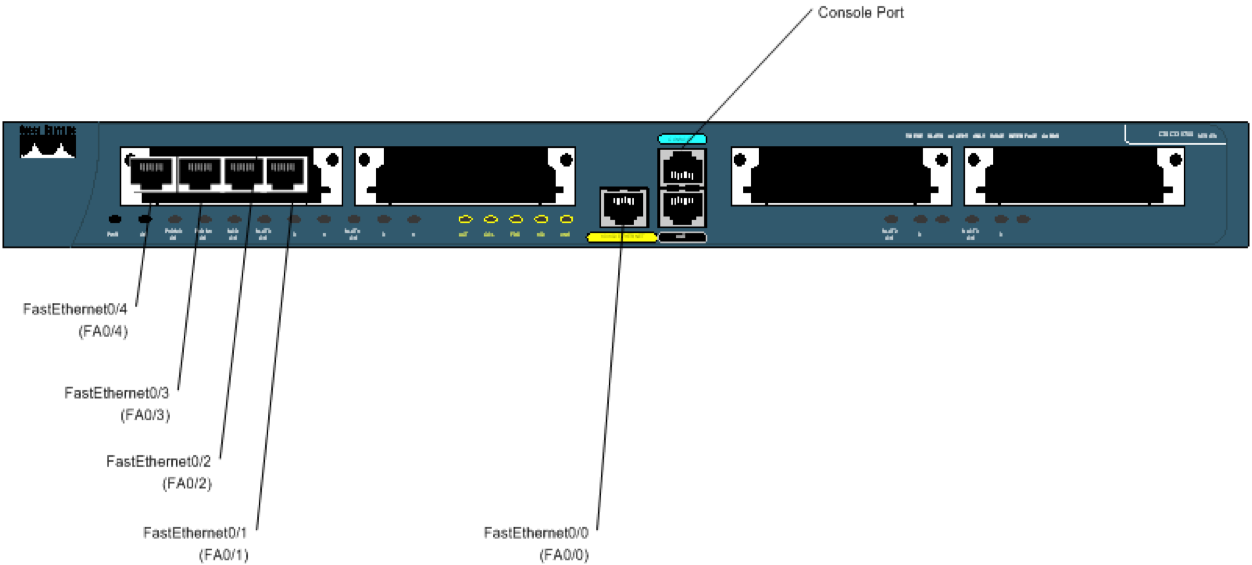
\includegraphics[width=\columnwidth]{graphics/cisco1760.png} 
      \caption{Cisco 1760} \label{fig:cisco1760}
    \end{center}
\end{figure}

The Cisco 1760 router has the following interfaces.
\begin{itemize}
	\item 1 Ethernet Port: FastEthernet0/0
	\item 1 Ethernet Switch Module: vlan1.
\end{itemize}

The 4 ports of the switch module have the following names \iface{FastEthernet0/1}, \iface{FastEthernet0/2}, \iface{FastEthernet0/3}, \iface{FastEthernet0/4}. Note that you can use the shorthand \iface{FA0/X} instead of writing \iface{FastEthernet0/X}.

The easiest way to configure the router is to:
\begin{itemize}
	\item Enable the onboard interface \iface{FA0/0} and give it an IP address.
	\item Turn on one of the ports of the switch module, we recommend you to always use \iface{FA0/1}.
	\item Enable the \iface{Vlan1} interface and assign it an IP address.
	\item We also recommend not changing any of the VLAN settings on the switch module.
\end{itemize}

In IOS this becomes:

\begin{cmdblock}
	Router1(config)# interface FastEthernet0/1
	Router1(config-if)# no shutdown
	Router1(config-if)# interface vlan1
	Router1(config-if)# ip address 10.0.2.1 255.255.255.0
	Router1(config-if)# no shutdown
\end{cmdblock}

Figure~\ref{fig:cisco-internal} shows a logical representation of the internal operation of the Cisco1760, and how the virtual interface \iface{Vlan1} can be configured with an IP address.

\begin{figure}[h!t]
    \begin{center}  
      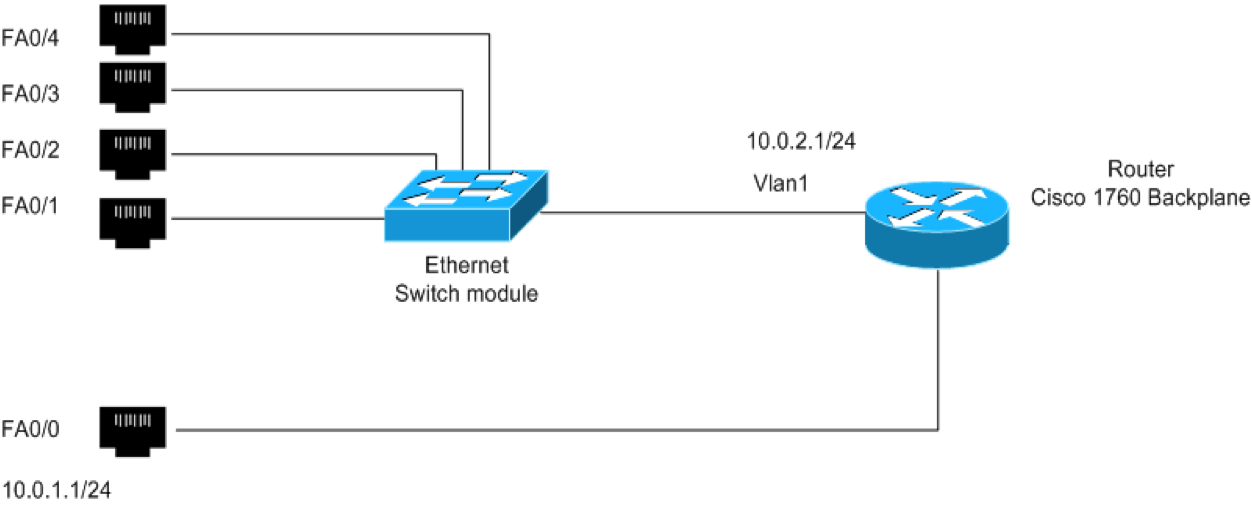
\includegraphics[width=\columnwidth]{graphics/cisco-internal.png} 
      \caption{Cisco 1760 Switch Module} \label{fig:cisco-internal}
    \end{center}
\end{figure}

The following exercises use basic commands from the Cisco IOS that are needed to configure a Cisco router.
\begin{enumerate}
	\item Start a minicom session on PC1 which is connected to Router1 with a serial cable.
	\item Configure Router1 with the IP addresses given in Table \ref{tab:lab3-network1}.
		\begin{cmdblock}
	Router1> enable
	Password: <enable secret>
	Router1# configure terminal
	Router1(config)# no ip routing
	Router1(config)# ip routing
	Router1(config)# interface FastEthernet0/0 
	Router1(config-if)# ip address 10.0.2.1 255.255.255.0 
	Router1(config-if)# no shutdown
	Router1(config-if)# interface FastEthernet0/1
	Router1(config-if)# no shutdown
	Router1(config-if)# interface vlan1
	Router1(config-if)# ip address 10.0.3.1 255.255.255.0 
	Router1(config-if)# no shutdown
	Router1(config-if)# end
		\end{cmdblock}
	\item When you are done, use the following command to check the changes you made to the router configuration, and save the output:
		\begin{cmdblock}
	Router1# show interfaces 
	Router1# show running-config
		\end{cmdblock}
	\item Analyze the output to ensure that you have configured the router correctly.
\end{enumerate}

\begin{questions}
	\q{2.C.1}{Include the output from Step 3 in your lab report.}
\end{questions}
	
	
\subsubsection{Exercise 2-d. Setting static routing table entries on a Cisco router}

Next you must add static routes to the routing table of Router1. The routing table must be configured so that it conforms to the network topology shown in Figure \ref{fig:lab3-network1} and Table \ref{tab:lab3-network1}.

The IOS command to configure static routing is \cmd{ip route}. The command can be used to show, clear, add or delete entries in the routing table. Below is a summary of the commands.

\boxinfo{The following can be executed in the privileged EXEC mode.:
	\begin{description}
		\item[\texttt{show ip route}]\hfill \\
			Display the contents of the routing table.
		\item[\texttt{clear ip route *}]\hfill \\
			Delete all routing table entries.
		\item[\texttt{show ip cache}]\hfill \\
			Display the routing cache.
	\end{description}
}

\boxinfo{The following can can be executed in the Global Configuration mode.
	\begin{description}
		\item[\texttt{ip route-cache}]\hfill \\
			Enable route caching. By default, route caching is enabled on a router.
		\item[\texttt{no ip route-cache}]\hfill \\
			Disable route caching.
		\item[\texttt{ip route destination mask gw\_address}]\hfill \\
			Add a static routing table entry to destination with netmask \cmd{mask}. The argument \cmd{gw\_address} is the IP address of the next hop router.
		\item[\texttt{ip route destination mask Iface}]\hfill \\
			Add a static routing table entry to destination with netmask \cmd{mask}. Here, the next hop information is the name of a network interface (e.g., \iface{FastEthernet0/0}).
		\item[\texttt{no ip route destination mask gw\_address no ip route destination mask Iface}]\hfill \\
			Delete the route table entry with \cmd{destination}, \cmd{mask}, and \cmd{gw\_address} or \cmd{Iface} from the routing table.
	\end{description}
}

We next show some examples for adding and deleting routing table entries in IOS. Compare these commands to the corresponding Linux commands in Part 2, Exercise 1-c. As in Linux, whenever an IP address is configured for a network interface, routing table entries for the directly connected network are added automatically.

The command for adding a route for the network prefix 10.21.0.0/16 with 10.11.1.4 as the next hop address is
\begin{cmdblock}
	Router1(config)#ip route 10.21.0.0 255.255.0.0 10.11.1.4 
\end{cmdblock}

The command to add a host route to IP address 10.0.2.31 with the next hop set to 10.0.1.21 is
\begin{cmdblock}
	Router1(config)#ip route 10.0.2.31 255.255.255.255 10.0.1.21
\end{cmdblock}

In IOS,a host route is identified by a 32-bit prefix. The command to add the IP address 10.0.4.4 as the default gateways is done with the command.
\begin{cmdblock}
     Router1(config) #ip route 0.0.0.0 0.0.0.0 10.0.4.4
\end{cmdblock}

Finally, commands to delete the above entries use the \cmd{no ip route} command.
\begin{cmdblock}
	Router1(config)# no ip route 10.21.0.0 255.255.0.0 10.11.1.4 
	Router1(config)# no ip route 10.0.2.31 255.255.255.255 10.0.1.21 
	Router1(config)# no ip route 0.0.0.0 0.0.0.0 10.0.4.4
\end{cmdblock}

\begin{enumerate}
	\item Display the content of the routing table with \cmd{show ip route}. Note the routing entries that are already present. Save the output.
	\item Add routing entries to Router1, so that the router forwards datagrams for the configuration shown in Figure \ref{fig:lab3-network1}. Routing entries should exist for the following networks:
		\begin{itemize}
			\item 10.0.1.0/24
			\item 10.0.2.0/24
			\item 10.0.3.0/24
		\end{itemize}
	\item Display the routing table again with \cmd{show ip route} and save the output.
\end{enumerate}

\begin{questions}	
	\q{2.D.1}{Include the saved output of the routing table from Step 1 and Step 2. Explain the fields of the routing table entries of the Cisco router. Explain how the routing table has changed from Step 1 to Step 3.}
\end{questions}

\newpage
\subsection{Finalizing and Exploring the Router Configuration}
If the configuration of PC2 and Router1 was done correctly, it is now possible to send IP datagrams between any two machines in the network shown in Figure \ref{fig:lab3-network1}. However, if the network is not configured properly, you need to debug and test your setup. The table below illustrates several common problems that may arise. Since it is impossible to cover all scenarios, network debugging is a crucial skill that you need to obtain for your lab experiments to work well.

\begin{table}[h!t]
	\centering
	\begin{tabular}{ | p{4cm} | p{4cm} | p{4cm} | }
		\hline
		\textbf{Problem} & \textbf{Possible Causes} &  \textbf{Debugging} \\ \hline
		Traffic does not reach destinations on local network & Network interface not configured correctly.& Verify the interface configuration with \cmd{show protocols} (in IOS) or \cmd{ifconfig} (in Linux) \\
		& & \\
		& Incorrectly connected, faulty, or loose cables. & Most interface cards and Ethernet hubs have green LED status lights. Check if the status lights are on. \\
		& & \\
		& & Verify the connection of the cables.\\
		& & \\
		& & Verify that no cross-over cables are used.\\ \hline
		Traffic reaches router, but is not forwarded to remote networks & IP forwarding is not enabled. & Use \cmd{show protocols} (in IOS) or look into \path{/proc/sys/net/ipv4 /ip\_forward} (in Linux) to display the forwarding status \\
		& & \\
		& Routing tables are not configured correctly. & Display routing tables with \cmd{show ip route} (in IOS) or \cmd{netstat -rn} (in Linux). Run \cmd{traceroute} between all hosts and routers. \\ \hline
		ICMP Request messages reaches destination, but ICMP Reply does not reach source & Routing tables are not correctly configured for the reverse path. & Display routing tables with \cmd{show ip route} (in IOS) or \cmd{netstat -rn} (in Linux). Run \cmd{ping} and \cmd{traceroute} in both directions. \\ \hline
		A change in the routing table has no effect on the flow of traffic. & The ARP cache has old entries. & Delete the ARP cache with \cmd{clear arp} (in IOS) or delete entries with \cmd{arp -d} (in Linux). \\ \hline
	\end{tabular}
\end{table}

\subsubsection*{Exercise 3-A. Finalizing the network setup}

Test the network configuration by issuing ping commands from each host and router to every other host and router. If some ping commands do not work, you need to modify the configuration of routers and hosts. If all ping commands are successful, the network configuration is correct, and you can proceed to the next step.

\subsubsection*{Exercise 3-B. Testing routes with traceroute}

\begin{enumerate}
	\item Start an Wireshark session on PC1.
	\item Execute a \cmd{traceroute} command from PC1 to PC4, and save the output.
		\begin{cmdblock}
	PC1% traceroute 10.0.3.41
		\end{cmdblock}
		Observe how \cmd{traceroute} gathers information on the route.
	\item Stop the traffic capture of Wireshark and save the traffic generated by the \cmd{traceroute} command.
	\item Save the routing table of PC1, PC4, PC2 and Router1.
\end{enumerate}

\begin{questions}
	\q{3.B.1}{Use the Wireshark output and the previously saved routing table to explain the operation of \cmd{traceroute}.}
\end{questions}
	
\subsubsection*{Exercise 3-C. Observe MAC addresses at a router}

When a router forwards an IP datagram from one Ethernet segment to another, it does not modify the IP destination address. However, the destination Ethernet address in the Ethernet header is modified at a router.

This exercise requires manipulations to the ARP cache. The \cmd{arp} command in Linux was covered in Lab 2. Below are the corresponding IOS commands for Cisco routers.

\boxinfo{The following can can be executed in the privileged EXEC mode:
	\begin{description}
		\item[\texttt{ip arp}]\hfill \\
			Display the contents of the ARP cache
		\item[\texttt{clear arp}]\hfill \\
			Delete the entire ARP cache
	\end{description}
}

\boxinfo{The following can can be executed in the Global Configuration mode:
	\begin{description}
	\item[\texttt{arp IPaddress}]\hfill \\
		Add an entry for \cmd{IPaddress} to the ARP cache
	\item[\texttt{no arp IPaddress}]\hfill \\
		Delete the ARP entry for \cmd{IPaddress} from the ARP cache
	\end{description}
}

\begin{enumerate}
	\item Erase all ARP entries on PC1, PC2, PC4 and Router1.
	\item Run Wireshark on both PC1 (interface \iface{eth0}) and PC4 (interface \iface{eth0}).
	\item Issue a \cmd{ping} command on PC1 to PC4.
		\begin{cmdblock}
	PC1% ping -c 5 10.0.3.41
		\end{cmdblock}
	\item Save the packet transmissions triggered by the \cmd{ping} command, including ARP requests, ARP reply, ICMP echo request, ICMP echo reply on both PC1 and PC4.
\end{enumerate}

\begin{questions}
	\q{3.C.1}{Determine the source and destination addresses in the Ethernet and IP headers, for the ICMP Echo Request messages that were captured at PC1.}
	\q{3.C.2}{Determine the source and destination addresses in the Ethernet and IP headers, for the ICMP Echo Request message that were captured at PC4.}
	\q{3.C.3}{Use your answers above to explain how the source and destination Ethernet and IP addresses are changed when a datagram is forwarded by a router.}
\end{questions}
	
\subsubsection*{Exercise 3-D. Multiple matches in the routing table}

A router or host uses a routing table to determine the next hop of the path of an IP datagram. In Linux, routing table entries are sorted in the order of decreasing prefix length, and are read from top to bottom. In this exercise, you determine how an IP router or Linux PC resolves multiple matching entries in a routing table.

\begin{enumerate}
	\item Add the following routes to the routing table of PC1:
		\begin{cmdblock}
	PC1% route add -net 10.0.0.0 netmask 255.255.0.0 gw 10.0.1.71
	PC1% route add -host 10.0.3.9 gw 10.0.1.81
		\end{cmdblock}
		From Exercise 1-C there should be a network route for the network prefix 10.0.3.0/24. If there is no such route, then add the following entry:
		\begin{cmdblock}
	PC1% route add -net 10.0.3.0 netmask 255.255.255.0 gw 10.0.1.61
		\end{cmdblock}
	\item Referring to the routing table, determine how many matches exist for the following IP addresses:
		\begin{cmdblock}
	10.0.3.9 
	10.0.3.14
	10.0.4.1
		\end{cmdblock}
	\item Start an Wireshark session on PC1, and issue the following ping commands from PC1:
		\begin{cmdblock}
	PC1% ping -c 1 10.0.3.9 
	PC1% ping -c 1 10.0.3.14 
	PC1% ping -c 1 10.0.4.1
		\end{cmdblock}

		Note that gateways with IP addresses 10.0.1.61, 10.0.1.71, and 10.0.1.81 do not exist. However, PC1 still sends ARP Request packets for these IP addresses.
	\item Save the output of Wireshark and PC1’s routing table.
\end{enumerate}

\begin{questions}
	\q{3.D}{Use the saved output to indicate the number of matches for each of the IP addresses above. Explain how PC1 resolves multiple matches in the routing table. Only include relevant output data in your report to support your analysis of the data.}
\end{questions}
	
\subsubsection*{Exercise 3-E. Default Routes}
\begin{enumerate}
	\item Delete the routing table entries added in Step 1 of Exercise 3-D above. (Otherwise, the entries interfere with the remaining exercises in this lab.)
	\item Add default routes on PC1 and PC2.
		\begin{itemize}
			\item On PC1, add a default route with PC2 as the default gateway.
			\item On PC2, add a default route with Router1 as the default gateway.
		\end{itemize}
	\item Start to capture traffic on PC1 (on \iface{eth0}) and PC2 (on both \iface{eth0} and \iface{eth1}) with Wireshark.
	\item Issue a \cmd{ping} command from PC1 to a host on a network that does not exist.
		\begin{cmdblock}
	PC1% ping -c 5 10.0.10.110
		\end{cmdblock}
	\item Save the Wireshark output.
\end{enumerate}

\begin{questions}
	\q{3.E.1}{What is the output on PC1, when the ping command is issued?}
	\q{3.E.2}{Determine how far the ICMP Echo Request message travels?}
	\q{3.E.3}{Which ICMP Echo Reply message returns to PC1?}
\end{questions}

\newpage
\subsection{Proxy ARP}
Proxy Address Resolution Protocol (Proxy ARP) is a method by which a router can forward traffic without using its routing table. Proxy ARP is a configuration option, where an IP router responds to ARP Requests that arrive from one of its connected networks for a host that is on another of its connected networks. Without Proxy ARP enabled, an ARP Request for a host on a different network is unsuccessful, since routers do not forward ARP packets to another network.

In this part, you explore how Proxy ARP enables routers to forward an IP datagram even though the sender of the datagram is not aware that the IP datagram should be forwarded to a router. Proxy ARP is enabled and disabled separately on each interface. In IOS, proxy ARP is enabled by default.

The commands to enable and disable Proxy ARP in the IOS Interface configuration mode are:
\begin{cmdblock}
	ip proxy-arp
	no ip proxy-arp
\end{cmdblock}

\subsubsection*{Exercise 4.}
\begin{enumerate}
	\item Erase the ARP table and the routing table of PC4.
	\item Set the netmask of PC4 to 255.0.0.0, so that PC4 assumes it belongs to network 10.0.0.0/8, instead of belonging to the network 10.0.3.0/24.
	\item Run Wireshark on PC4 (\iface{eth0}), PC2 (\iface{eth1}), and PC1 (\iface{eth0}). Set a display or capture filter to only display ICMP and ARP packets.
	\item Issue a \cmd{ping} from PC4 to PC1:
		\begin{cmdblock}
	PC4% ping -c 2 10.0.1.11
		\end{cmdblock}
		Explore the captured data and interpret the outcome.
		Even though PC4 had no default routing entry in its table for Router1, it was still able to connect to PC1, i.e., you should not observe a ``network unreachable'' error message.
	\item Save the ARP table of PC4 and the packets captured by Wireshark on the hosts.
	\item Explore the captured data and interpret the outcome.
	\item Now, disable Proxy ARP on both interfaces of Router1. Is it still feasible to issue a ping from PC4 to PC1?
	\item Reset the network mask of PC4 to its original value of 255.255.255.0. Then, re-enable Proxy ARP on Router1.
\end{enumerate}

\begin{questions}
	\q{4.1}{Use the captured data to explain the outcome of the exercise. Use the data to explain how Proxy ARP allowed PC4 to communicate with PC1. Include only relevant data from your saved output.}
\end{questions}

\newpage
\subsection{ICMP Route Redirect}
ICMP route redirect messages are sent from a router to a host, when a datagram should have been forwarded to a different router or interface. In Linux, an ICMP Route Redirect message updates the routing cache, but not the routing table.

Both the routing cache and the routing table contain information for forwarding traffic. When a Linux system performs a routing table lookup, it first inspects the routing cache. If no matching entry is found in the cache, Linux performs a lookup in the routing table. After each routing table lookup, an entry is added to the routing cache. The routing cache does not aggregate table entries, and there is a separate entry for each destination IP address. As a consequence, a lookup in the routing cache does not require a longest prefix match. An entry in the routing cache is deleted if it has not been used for some time, usually after 10 minutes. When an ICMP redirect message arrives, an entry is added to the routing cache, but no update is performed to the routing table.

\boxinfo{The following are the commands to display the contents of the routing cache:
	\begin{description}
	\item[\texttt{route -C}]\hfill \\
		In Linux
	\item[\texttt{show ip cache}]\hfill \\
		In IOS
	\end{description}
}

In this part of the lab, you use three Cisco routers. Figure \ref{fig:lab3-network2} and Table \ref{tab:lab3-network2} describe the network configuration for the exercises below.

\begin{figure}[h!t]
	\centering
	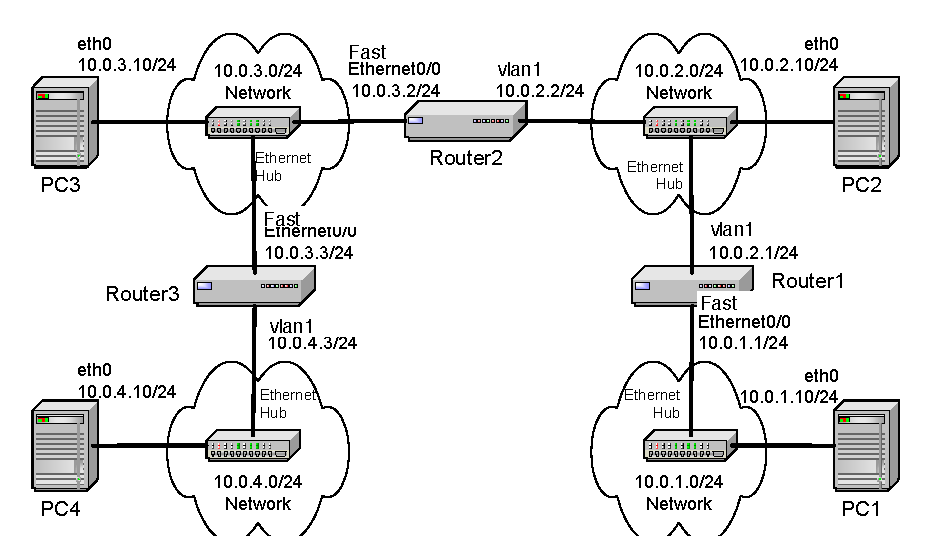
\includegraphics[width=\linewidth]{graphics/lab3-network2-updated.pdf}	
	\caption{Network configuration for Part 5}
	\label{fig:lab3-network2}
\end{figure}

\begin{table}[h!t]
	\centering
	\begin{tabular}{| c | c | c |}	
		\hline
		\textbf{Cisco Router} & \textbf{FastEthernet0/0} & \textbf{vlan1} \\ \hline
		Router1 & 10.0.1.1/24 & 10.0.2.1/24 \\
		Router2 & 10.0.3.2/24 & 10.0.2.2/24 \\
		Router3 & 10.0.3.3/24 & 10.0.4.3/24 \\ \hline
		\textbf{Linux PC} & \textbf{eth0} & \textbf{eth1} \\ \hline
		PC1 & 10.0.1.10/24 & Disabled \\ 
		PC2 & 10.0.2.10/24 & Disabled \\
		PC3 & 10.0.3.10/24 & Disabled \\
		PC4 & 10.0.4.10/24 & Disabled \\ \hline
	\end{tabular}
	\caption{IP addresses for Part 5}
	\label{tab:lab3-network2}
\end{table}

\subsection*{Exercise 5.}
In the network shown in Figure \ref{fig:lab3-network2}, when PC2 sends datagrams with destination 10.0.3.10 (PC3) to 10.0.2.1 (Router1), as opposed to 10.0.2.2 (Router2), then Router1 sends an ICMP Route Redirect message to PC2. The ICMP Route Redirect informs PC2 that it should send datagrams with destination 10.0.3.10 to Router2 instead.

In this exercise, you create the above scenario. First, you will trigger the transmission of an ICMP Route Redirect message and subsequently observe a change to the routing cache.
\begin{enumerate}
	\item Connect the Ethernet interfaces of the routers and the hosts to the hubs as shown in Figure \ref{fig:lab3-network2}.
	\item Delete all routing table entries and all ARP cache entries on all PCs and on Router 1. 
		\begin{itemize}
			\item Delete the routing cache on PC1 with the command:
				\begin{cmdblock}
	PC1% echo "1" > /proc/sys/net/ipv4/route/flush
				\end{cmdblock}
			\item Delete all static routes on Router 1 with the following commands: 
				\begin{cmdblock}
	Router1(config)# no ip routing
	Router1(config)# ip routing
				\end{cmdblock}
			\item Build a new static routing entry on Router1 for network prefix 10.0.3.0/24 as follows:
				\begin{cmdblock}
	Router1(config)# ip route 10.0.3.0 255.255.255.0 10.0.2.2
				\end{cmdblock}
		\end{itemize}
	\item Setup the routing table of PC2 in such a way that it provokes the transmission of an ICMP Route Redirect message as discussed above.
	\item Save the contents of the routing table and the routing cache of Router1, Router2, and PC2.
	\item Use Wireshark to capture the ICMP messages being sent, and issue a ping from PC2 to PC3:
		\begin{cmdblock}
	PC2% ping -c 5 10.0.3.10
		\end{cmdblock}
	\item Save the network traffic and the contents of the routing table and the routing cache after the ICMP Route Redirect messages.
	\item Wait a few minutes and check the contents of the routing cache again. Save the output.
\end{enumerate}

\begin{questions}
	\q{5.1}{Is there a difference between the contents of the routing table and the routing cache immediately after the ICMP Route Redirect message?}
	\q{5.2}{When you viewed the cache a few minutes later, what did you observe?}
	\q{5.3}{Describe how the ICMP Route Redirect works using the output you saved. Include only relevant data from your saved output to support your explanations.}
	\q{5.4}{Explain how Router1, in the above example, knows that datagrams destined to network 10.0.3.10 should be forwarded to 10.0.2.2?}
\end{questions}

\newpage
\subsection{Routing Loops}

A potential problem when setting routing tables manually is that routing loops may occur. In this part of the lab, you intentionally configure a routing loop in the configuration of the routing table and observe what happens to network traffic in such a situation.

\begin{figure}[h!t]
	\centering
	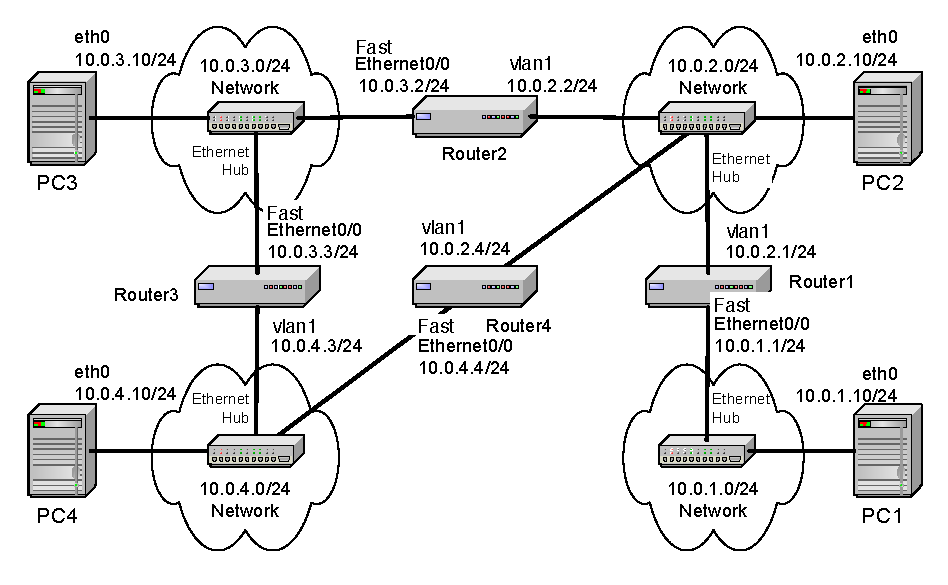
\includegraphics[width=\linewidth]{graphics/lab3-network3-updated.pdf}	
	\caption{Network configuration for Part 6}
	\label{fig:lab3-network3}
\end{figure}

\begin{table}[h!t]
	\centering
	\begin{tabular}{| c | c | c |}	
		\hline
		\textbf{Cisco Router} & \textbf{FastEthernet0/0} & \textbf{vlan1} \\ \hline
		Router4 & 10.0.4.4/24 & 10.0.2.4/24 \\ \hline
	\end{tabular}
	\caption{IP addresses for Part 6}
	\label{tab:lab3-network3}
\end{table}

\subsubsection*{Exercise 6.}
\begin{enumerate}
	\item Add Router4 to the network topology of Part 5 and configure the interfaces as shown in Figure \ref{fig:lab3-network3} and Table \ref{tab:lab3-network3} above.
	\item Configure the routing tables of Router2, Router3 and Router4, so that an ICMP Echo Request message generated by a ping from PC4 to PC1 creates an infinite loop. Issue a \cmd{traceroute} to verify that a loop exists:
		\begin{cmdblock}
	PC4% traceroute 10.0.1.10
		\end{cmdblock}
		You should observe that the traced path is a loop.
	\item Start Wireshark sessions on PC2, PC3, and PC4.
	\item Issue a ping from PC4 to
		\begin{cmdblock}
	PC4% ping -c 1 10.0.1.10
		\end{cmdblock}
		Observe in Wireshark that the same ICMP Echo Request message is looping.
	\item Save the routing tables of Router2, Router3 and Router4. Count the number of times you see the ICMP Echo Request message, as captured by Wireshark on PC4. Save at least two of these ICMP Echo Request messages for the lab report.
\end{enumerate}

\begin{questions}
	\q{6.1}{Are the two ICMP packets that you saved identical? If not, what is different? Include the packet data in your lab report to substantiate your claims.}
	\q{6.2}{Why does the ICMP Echo Request packet not loop forever in the network?}
\end{questions}
	
\newpage	
\subsection{Network Prefixes and Routing}
In this exercise you study the role that network prefixes (netmasks) play when hosts determine if a datagram can be directly delivered or if it must be sent to a router.

This part uses the network setup shown in Figure \ref{fig:lab3-network4}. The network includes one router, four hosts and two hubs. The IP addresses of all devices are given in Table \ref{tab:lab3-network4}. Here, each host has only a default route. In other words, the routing table at a host only knows about the directly connected networks and the default gateway.

\begin{figure}[h!t]
	\centering
	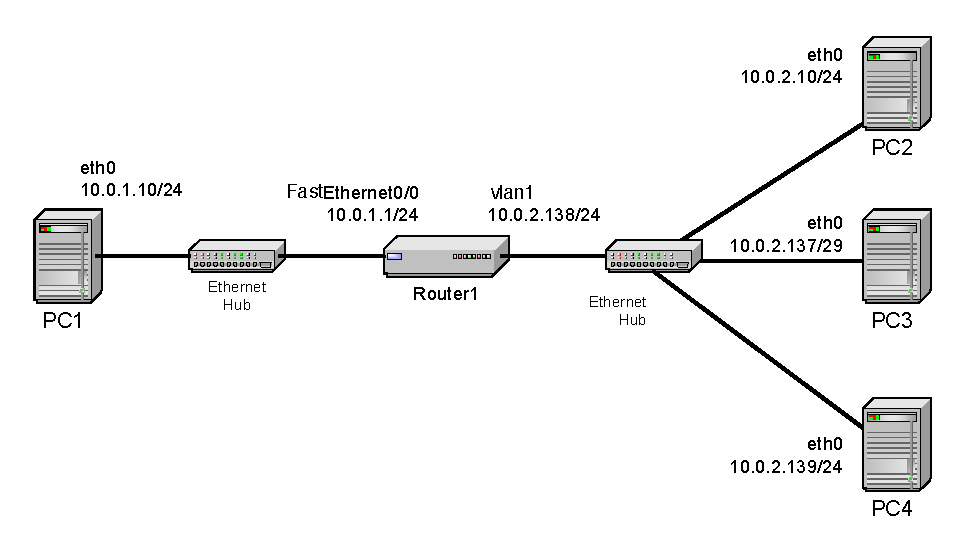
\includegraphics[width=\linewidth]{graphics/lab3-network4-updated.pdf}	
	\caption{Network configuration for Part 7}
	\label{fig:lab3-network4}
\end{figure}

\begin{table}[h!t]
	\centering
	\begin{tabular}{| c | c | c |}	
		\hline
		\textbf{Linux PC} & \textbf{eth0} & \textbf{eth1} \\ \hline
		PC1 & 10.0.1.10/24 & Disabled \\ 
		PC2 & 10.0.2.10/24 & Disabled \\
		PC3 & 10.0.2.137/29 & Disabled \\
		PC4 & 10.0.2.139/24 & Disabled \\ \hline
		\textbf{Cisco Router} & \textbf{FastEthernet0/0} & \textbf{vlan1} \\ \hline
		Router1 & 10.0.1.1/24 & 10.0.2.138/24 \\ \hline
	\end{tabular}
	\caption{IP addresses for Part 7}
	\label{tab:lab3-network4}
\end{table}

\subsubsection{Exercise 7.}
In this exercise, you explore how hosts that are connected to the same local area network, but that have different network addresses or netmasks, communicate or fail to communicate.

\begin{enumerate}
	\item Configure the hosts and the router to conform to the topology shown in Figure \ref{fig:lab3-network4}, using the IP addresses as given in Table \ref{tab:lab3-network4}.
		Note that PC2, PC3, and PC4 have different network addresses and different netmasks.
	\item Add Router1 as default gateway on all hosts. For example, for PC1, the command is:
		\begin{cmdblock}
	PC1% route add default gw 10.0.1.1
		\end{cmdblock}
	\item Issuing ping commands from PC1:
		\begin{enumerate}[label=\alph*.,leftmargin=3em]
			\item Clear the ARP table on all hosts.
			\item Start Wireshark on PC1 and on PC4, and set the capture filter to capture ICMP and ARP packets only.
			\item Check the ARP tables, routing tables and routing caches of each host. Save the output. (Make a note that these are the table entries from Step 3 before the ping is issued.)
			\item Issue a \cmd{ping} command from PC1 to PC2 and PC3 
				\begin{cmdblock}
	PC1% ping -c 2 10.0.2.10
	PC1% ping -c 2 10.0.2.137
				\end{cmdblock}
			\item Save the ARP tables, routing tables and routing caches of each host (Make a note that these are the table entries from Step 3 after the ping is issued.)
			\item Save the output of the ping command at PC1 and the output of Wireshark on PC1 and PC4.
		\end{enumerate}
	\item Issuing a ping command from PC3 to PC4:
		\begin{enumerate}[label=\alph*.,leftmargin=3em]
			\item Clear the ARP table on all hosts.
			\item Start Wireshark on PC3, and set the capture filter to capture ICMP and ARP packets only.
			\item Check the ARP tables, routing tables and routing caches of each host. Save the output. (Make a note that these are the table entries from Step 4 before the ping is issued.)
			\item Issue a \cmd{ping} from PC3 to PC4. 
				\begin{cmdblock}
	PC3% ping -c 3 10.0.2.139
				\end{cmdblock}
			\item Save the ARP tables, routing tables and routing caches of PC3 (Make a note that these are the table entries from Step 4 after the ping is issued.)
			\item Save the output of the \cmd{ping} command and the output of Wireshark on PC3.
		\end{enumerate}
	\item Repeat Step 4, but this time issue a ping from PC3 to PC2. Note that once an entry is made in the routing cache, you cannot repeat the above experiment and obtain the same results; you have to wait until the routing cache is reset (which take some time).
\end{enumerate}

\begin{questions}
	\q{7.1}{Explain what you observed in Steps 3, 4 and 5. Use the saved data to support your answers. Provide explanations of the observations. Try to explain each observed phenomenon, e.g., if you observe more ICMP Echo Requests than ICMP Echo Replies, try to explain the reason.}
	\q{7.2}{If PC3 had no default entry in its table, would you have seen the same results? Explain for each of the pings above what would have been different.}
\end{questions}

\setcounter {chapter} {3}
%%!TEX root = labo.tex

\chapter{Dynamic Routing Protocols (RIP and OSPF)}

What you will learn in this lab:
\begin{itemize}
	\item How to configure the routing protocols RIP, OSPF, and BGP on a Linux PC and a Cisco router.
	\item How those routing protocols update the routing tables after a change in the network topology.
	\item How the count-to-infinity problem in RIP can be avoided.
	\item How OSPF achieves a hierarchical routing scheme through the use of multiple areas.
\end{itemize}

\newpage
\setsession{prelab4}
\section{Prelab 4}\label{sec:prelab4}
%!TEX root = labo.tex

\subsubsection*{Routing protocols}
\begin{itemize}
	\item \emph{Distance Vector and Link State Routing Protocols}: Go to the website \url{http://docwiki.cisco.com/wiki/Internetworking_Technology_Handbook} and read the article about dynamic routing protocols. Review your knowledge of interdomain and intradomain routing, distance vector routing, and link state routing.
	\item \emph{Zebra}: Go to the website of the Zebra fork Quagga at \url{http://www.nongnu.org/quagga/} and study the information on the Quagga routing protocol software for Linux systems. Also find and read the man pages on zebra, ripd, ospfd and bgpd. Note: Quagga is a fork of the GNU Zebra project.
	\item \emph{RIP}: Read the overview of the Routing Information Protocol (RIP) and study the commands to configure RIP on a Cisco router at \url{http://www.routeralley.com/guides/rip.pdf}.
	\item \emph{OSPF}: Read the overview of Open Shortest Path First (OSPF) routing protocol and study the commands to configure OSPF on a Cisco router at \url{http://www.routeralley.com/guides/ospf.pdf}.
\end{itemize}

\newpage
\subsubsection*{Prelab Questions}

\begin{questions}
	\q{1}{Provide the command that configures a Linux PC as an IP router (see Lab 3).}
	\q{2}{What are the main differences between a distance vector routing protocol and a link state routing protocol? Give examples for each type of protocol.}
	\q{3}{What are the differences between an intradomain routing protocol (also called interior gateway protocol or IGP) and an interdomain routing protocol (also called exterior gateway protocol or EGP)? Give examples for each type of protocol.}
	\q{4}{Which routing protocols are supported by the software package Zebra?}
	\q{5}{In the Zebra software package, the processes ripd, ospfd, and bgpd deal, respectively, with the routing protocols RIP, OSPF, and BGP. Which role does the process zebra play?}
	\q{6}{Describe how a Linux user accesses the processes of Zebra (zebra, ripd, ospfd, bgpd) processes to configure routing algorithm parameters?}
	\q{7}{What is the main difference between RIP version 1 (RIPv1) and RIP version 2 (RIPv2)?}
	\q{8}{Explain what it means to ``run RIP in passive mode''.}
	\q{9}{Explain the meaning of ``triggered updates'' in RIP.}
	\q{10}{Explain the concept of split-horizon in RIP?}
	\q{11}{What is an autonomous system (AS)? Which roles do autonomous systems play in the Internet?}
	\q{12}{What is the AS number of your institution? Which autonomous system has AS number 1?}
	\q{13}{Explain the terms: Stub AS, Multi-homed AS and Transit AS?}
\end{questions}


\newpage
\setsession{lab4}
\section{Lab 4}\label{sec:lab4}

In the previous lab, you learned how to configure routing table entries manually. This was referred to as static routing. The topic of Lab 4 is dynamic routing, where dynamic routing protocols (from now on, called routing protocols) set the routing tables automatically without human intervention. Routers and hosts that run a routing protocol, exchange routing protocol messages related to network paths and node conditions, and use these messages to compute paths between routers and hosts.

Most routing protocols implement a shortest-path algorithm, which, for a given set of routers, determines the shortest paths between the routers. Some routing protocols allow that each network interface be assigned a cost metric. In this case, routing protocols compute paths with least cost. Based on the method used to compute the shortest or least-cost paths, one distinguishes distance vector and link state routing protocols. In a distance vector routing protocol, neighbouring routers send the content of their routing tables to each other, and update the routing tables based on the received routing tables. In a link state routing protocol, each router advertises the cost of each of its interfaces to all routers in the network. Thus, all routers have complete knowledge of the network topology, and can locally run a shortest-path (or least-cost) algorithm to determine their own routing tables.

The notion of an autonomous system (AS) is central to the understanding of routing protocols on the Internet. An autonomous system is a group of IP networks under the authority of a single administration, and the entire Internet is carved up into a large number of autonomous systems. Examples of autonomous systems are the campus network of a university and the backbone network of a global network service provider. Each autonomous system is assigned a globally unique identifier, called the AS number. On the Internet, dynamic routing within an autonomous system and between autonomous systems is handled by different types of routing protocols. A routing protocol that is concerned with routing within an autonomous system is called an intradomain routing protocol or interior gateway protocol (IGP). A routing protocol that determines routes between autonomous systems is called an interdomain routing protocol or exterior gateway protocol (EGP).

In this lab, you study the two most common intradomain protocols, namely, the Routing Information Protocol (RIP) and the Open Shortest Path First (OSPF) protocol. Parts 1-3 of this lab deal with RIP, and Parts 4-5 are about OSPF. 
% In Part 7, you are exposed to a few features of the Border Gateway Protocol (BGP), which is the interdomain routing protocol of the Internet.

This lab uses two different network configurations. The first network configuration, shown in Figure \ref{fig:lab4-network1}, is used in Parts 1-2, and is modified in Part 3 (Figure \ref{fig:lab4-network1-part3}). The network configuration in Parts 4 and 5 is shown in Figure \ref{fig:lab4-network2}.

\newpage
\subsection{Configuring RIP on a Cisco router}

This lab starts with the same network topology as used in Part 5 of Lab 3. Different from Lab 3, where the routing tables were configured manually, here you run the routing protocol RIP to perform the same task. In Part 1, you configure RIP on the Cisco routers. In Part 2, you configure RIP on the Linux PCs.

RIP is one of the oldest dynamic routing protocols on the Internet that is still in use. This lab uses the latest revision of RIP, RIPv2 (RIP version 2). RIP is an intradomain routing protocol that uses a distance vector approach to determine the paths between routers. RIP minimizes the number of hops of each path, where each point-to-point link or LAN constitutes a hop.

Each RIP enabled router periodically sends the content of its routing table to all its neighbouring routers in an update message. For each routing table entry, the router sends the destination (host IP address or network IP address) and the distance to that destination measured in hops. When a router receives an update message from a neighbouring router, it updates its own routing table.

Figure \ref{fig:lab4-network1} and Table \ref{tab:lab4-network1} describe the network configuration for this part of the lab.

\begin{figure}[ht]
	\centering
	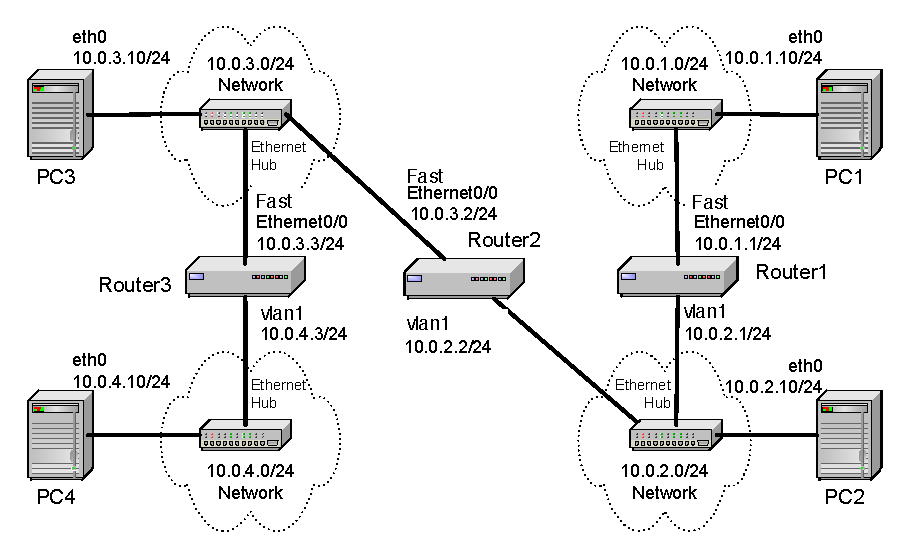
\includegraphics[width=\linewidth]{graphics/lab4-network1-updated.pdf}	
	\caption{Network configuration for Parts 1 and 2.}
	\label{fig:lab4-network1}
\end{figure}

\begin{table}[h!t]
	\centering
	\begin{tabular}{| c | c | c |}	
		\hline
		\textbf{Linux PC} & \textbf{eth0} & \textbf{eth1} \\ \hline
		PC1 & 10.0.1.10/24 & Disabled \\ 
		PC2 & 10.0.2.10/24 & Disabled \\
		PC3 & 10.0.3.10/24 & Disabled \\
		PC4 & 10.0.4.10/24 & Disabled \\ \hline
		\textbf{Cisco Router} & \textbf{FastEthernet0/0} & \textbf{vlan1} \\ \hline
		Router1 & 10.0.1.1/24 & 10.0.2.1/24 \\
		Router2 & 10.0.3.2/24 & 10.0.2.2/24 \\
		Router3 & 10.0.3.3/24 & 10.0.4.3/24 \\ \hline
	\end{tabular}
	\caption{IP addresses}
	\label{tab:lab4-network1}
\end{table}

\subsubsection*{Exercise 1. Configuring RIP on Cisco routers}

Configure all three Cisco routers to run the routing protocol RIP. Once the configuration is completed, all Cisco routers can issue ping commands to each other. Below, we give a brief overview of the basic commands used to configure RIP on a Cisco router.

The following can can be executed in the Global Configuration mode.

\begin{itemize}
	\item Enable the routing protocol RIP on the local router, and enters the router configuration mode from the following prompt:
		\begin{cmdblock}
	Router1(config-router)#
		\end{cmdblock}
		You return from the router configuration command to the global configuration command by typing the command \cmd{exit}.
		\begin{cmdblock}
	router rip
		\end{cmdblock}
	\item Disable RIP on the local router.
		\begin{cmdblock}
	no router rip
		\end{cmdblock}
\end{itemize}

The following can can be executed in the Privileged EXEC mode.

\begin{itemize}
	\item Enable a debugging mode where the router displays a message for each received RIP packet.
		\begin{cmdblock}
	debug ip rip
		\end{cmdblock}
	\item Disable the debugging feature
		\begin{cmdblock}
no debug ip rip
		\end{cmdblock}
\end{itemize}

The following can can be executed in the Router Configuration mode.

\begin{itemize}
	\item Associate the network IP address \emph{Netaddr} with RIP. RIP sends updates only on interfaces where the network address has been associated with RIP.
		\begin{cmdblock}
network Netaddr
		\end{cmdblock}
	\item Disable RIP for the specified network address.
		\begin{cmdblock}
	no network Netaddr
		\end{cmdblock}
	\item Set the interface \emph{Iface} in RIP passive mode. On an interface in passive mode, the router processes incoming RIP packets, but does not transmit RIP packets.
		\begin{cmdblock}
	passive-interface Iface
		\end{cmdblock}
	\item Enable active mode on interface \emph{Iface}. This means that RIP packets are transmitted on this interface.
		\begin{cmdblock}
	no passive-interface Iface
		\end{cmdblock}
	\item Increase the metric (hop count) of incoming RIP packets that arrive on interface \emph{Iface} by \emph{value}, where \emph{value} is a number.
		\begin{cmdblock}
	offset-list 0 in value Iface
		\end{cmdblock}
	\item Increase the metric of outgoing RIP packets that are sent on interface \emph{Iface} by \emph{value}.
		\begin{cmdblock}
	offset-list 0 out value Iface
		\end{verbatim}
	\item Disable the specified offset-list command for incoming RIP packets.
		\begin{cmdblock}
	no offset-list 0 in value Iface
		\end{cmdblock}
	\item Disable the specified offset-list command for outgoing RIP packets.
		\begin{cmdblock}
	no offset-list 0 out value Iface
		\end{cmdblock}
	\item Set the RIP version to RIPv2.
		\begin{cmdblock}
	version 2
		\end{cmdblock}
	\item Set the values of the timers in the RIP protocol. The timers are measured in seconds.
		\begin{cmdblock}
	timers basic update invalid hold-down flush
		\end{cmdblock}
		\begin{description}
			\item [\texttt{update}]: The time interval between transmissions of RIP update messages (Default: 30 sec).
			\item [\texttt{invalid}]: The time interval after which a route, which has not been updated, is declared invalid (Default: 180 sec).
			\item [\texttt{hold-down}]: Determines how long after a route has been updated as unavailable, a router will wait before accepting a new route with a lower metric. This introduces a delay for processing incoming RIP packets with routing updates after a link failure (Default: 180 sec).
			\item [\texttt{flush}]: The amount of time that must pass before a route that has not been updated is removed from the routing table (Default: 240 sec).
		\end{description}
		Example:
		\begin{cmdblock}
	Router1(config-router)# timers basic 30 180 180 240
		\end{cmdblock}
	\item Set the router to not perform triggered updates, when the next transmission of routing updates is due in time. If time is set to the same value as the update timer, then triggered updates are disabled. In RIP, a triggered update means that a router sends a RIP packet with a routing update, whenever one of its routing table entries changes.
		\begin{cmdblock}
	flash-update-threshold time
		\end{cmdblock}
\end{itemize}

\begin{enumerate}
	\item Connect the the Linux PCs and the Cisco routers as shown in Figure \ref{fig:lab4-network1}. The PCs and routers are connected with Ethernet hubs.
	\item Verify that the serial interfaces of the PCs are connected to the console port of the routers. PC1 should be connected to Router1, PC2 to Router2, and so on. Once the serial cables are connected, establish a minicom session from each PC to the connected router.
	\item On Router1, Router2, and Router3, configure the IP addresses as shown in Table \ref{tab:lab4-network1}, and enable the routing protocol RIP. The commands to set up Router1 are as follows:
		\begin{cmdblock}
	Router1> enable Password: <enable secret>
	Router1# configure terminal
	Router1(config)# no ip routing
	Router1(config)# ip routing
	Router1(config)# router rip
	Router1(config-router)# version 2 
	Router1(config-router)# network 10.0.0.0 
	Router1(config-router)# interface FastEthernet0/0 
	Router1(config-if)# no shutdown
	Router1(config-if)# ip address 10.0.1.1 255.255.255.0 
	Router1(config-if)# interface FastEthernet0/1 
	Router1(config-if)# no shutdown
	Router1(config-if)# interface vlan1
	Router1(config-if)# no shutdown
	Router1(config-if)# ip address 10.0.2.1 255.255.255.0 
	Router1(config-if)# end
	Router1# clear ip route *
		\end{cmdblock}
		The command \cmd{no ip routing} is used to reset all previous configurations related to routing (RIP, OSPF, etc). The command \cmd{clear ip route *} deletes all entries in the routing table. Make sure that all static routing entries are removed, since, in IOS, RIP does not overwrite static routing entries.
	\item After you have configured the routers, check the routing table at each router by typing
		\begin{cmdblock}
	Router1# show ip route
		\end{cmdblock}
		Each router should have four entries in the routing table: two entries for directly connected networks, and two other entries for remote networks that were added by RIP.
	\item From each router, issue a ping command to the IP addresses of interfaces \iface{FastEthernet0/0} and \iface{vlan1} on all remote routers. For example, to issue a ping from Router1 to interface \iface{FastEthernet0/0} on Router2, type
		\begin{cmdblock}
	Router1# ping 10.0.3.2
		\end{cmdblock}
\end{enumerate}

Once you can successfully contact the IP addresses of all routers, proceed to the next exercise.

\newpage
\subsection{Configuring RIP on a Linux PC}

In this part of the lab, you continue with the network configuration in Figure \ref{fig:lab4-network1} and Table \ref{tab:lab4-network1}, and configure RIP on the Linux PCs.

In Figure \ref{fig:lab4-network1}, all Linux PCs are set up as hosts. Since hosts do not perform IP forwarding, they need not send routing messages. Therefore, when a routing protocol is configured on a host, the protocol is set to run in passive mode, where a host receives and processes incoming routing messages, but does not transmit routing messages. (We note that, normally, routing protocols are not enabled on hosts. Instead, one generally configures a static routing table entry for the default gateway. Obviously, when a routing protocol is enabled, there is no need to configure a default gateway.)

The configuration of routing protocols on Linux PCs in Lab 4 is done with the routing software package Quagga. Before starting the exercise, we give a brief tutorial on the Quagga software package. The tutorial focuses on the features used in the lab exercises and omits many interesting features of Zebra.

\subsubsection*{An Introduction to Quagga}

Quagga is a software package that manages the routing tables of a Linux system, and that provides the ability to execute a variety of routing protocols. For this course we make use of Quagga, which is a fork of the GNU Zebra project and while the project has a new name, many of the references to Zebra still remain, e.g. there is still a \cmd{zebra} control process.

The Quagga architecture, shown in Figure \ref{fig:quagga}, consists of a set of processes. The process \cmd{zebra} updates the routing tables and exchanges routes between different routing protocols. Each routing protocol has a separate process, and each routing process can be started, stopped, configured, and upgraded independently of the other routing processes. The process \cmd{zebra} must be invoked prior to starting and configuring any of the routing protocols. The routing processes used in this lab and the routing protocols they manage are shown in table \ref{tab:quagga}.

\begin{table}[h!t]
	\centering
	\begin{tabular}{| l l |}	
		\hline
		\textbf{Routing Process} & \textbf{Routing Protocol}\\ \hline
		ripd & RIPv1 and RIPv2 \\
		ospfd & OSPFv2 (Version 2) \\ \hline
	\end{tabular}
	\caption{Quagga routing processes used for this lab.}
	\label{tab:quagga}
\end{table}

\begin{figure}[h]
	\centering
	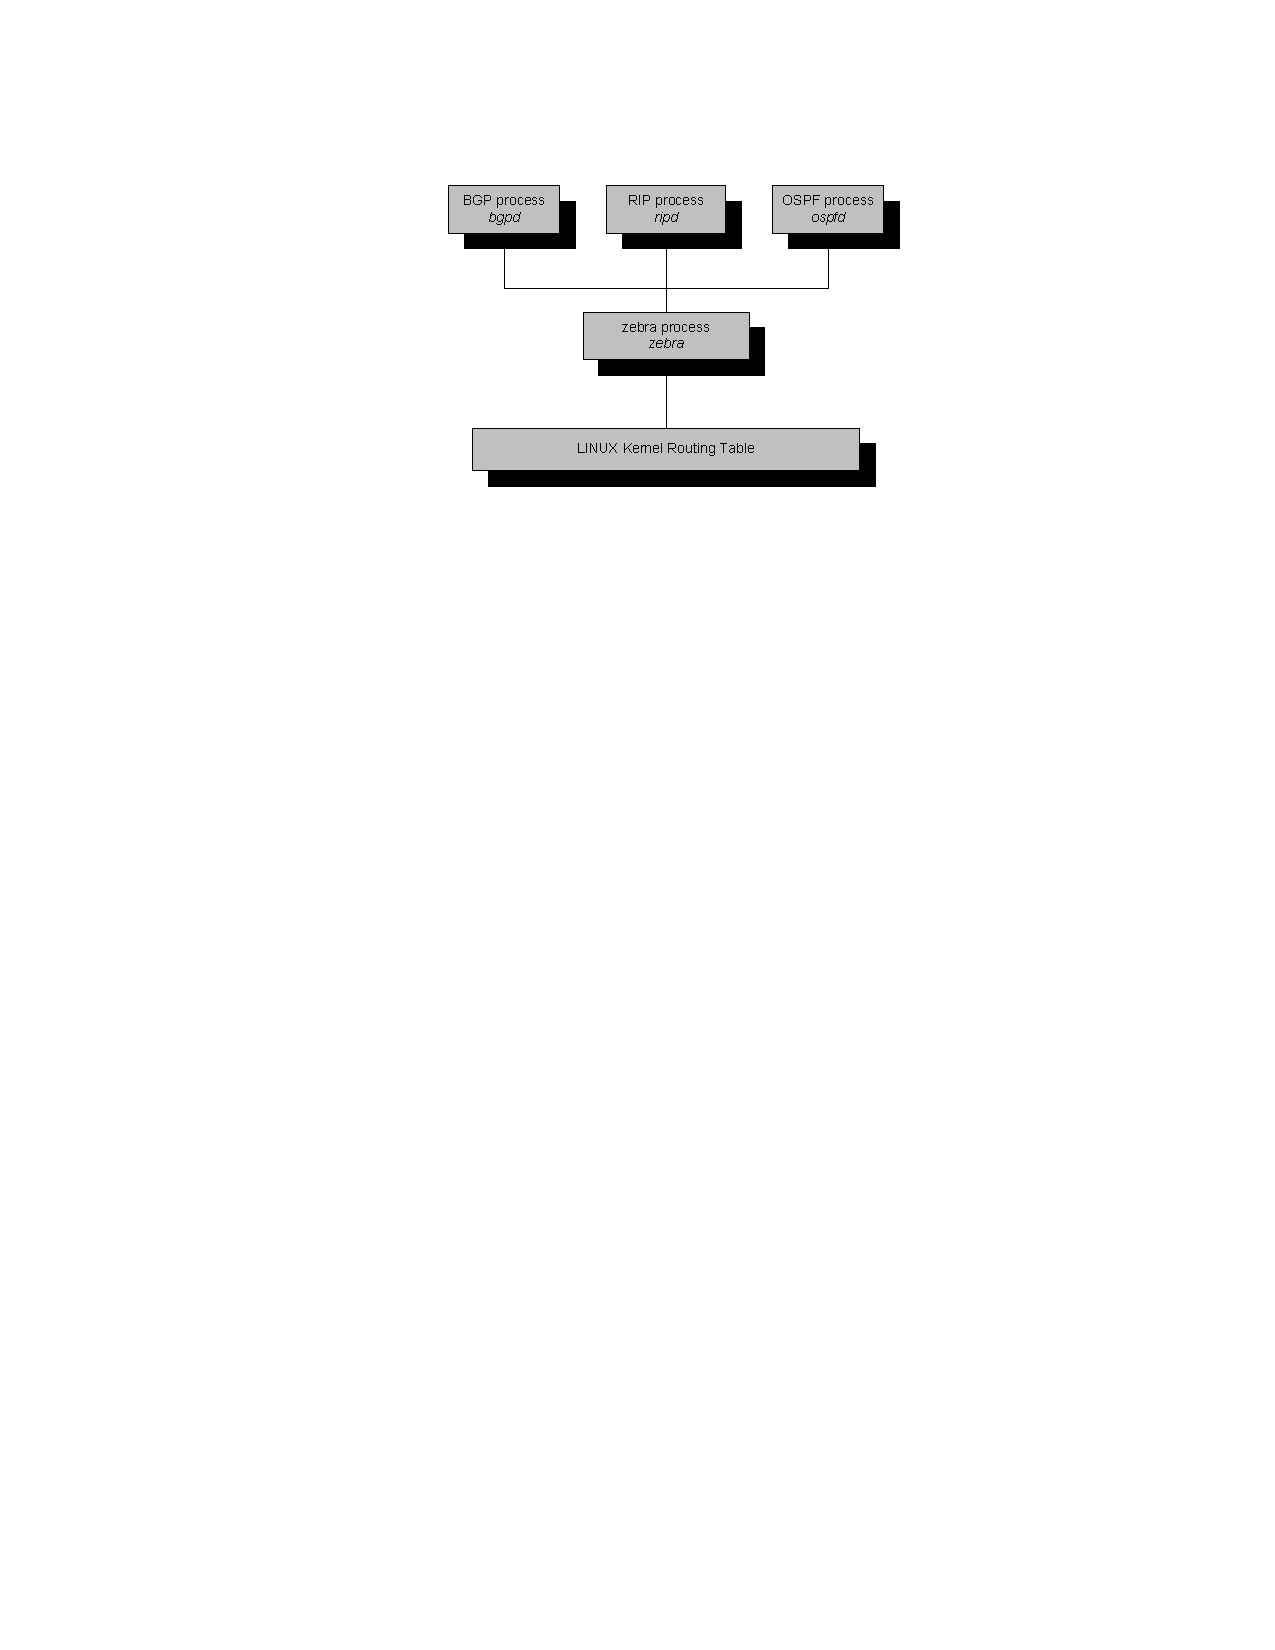
\includegraphics[width=0.7\linewidth]{graphics/quagga.pdf}	
	\caption{Quagga processes}
	\label{fig:quagga}
\end{figure}

\begin{enumerate}[label=\textbf{(\alph*)},labelindent=0em]
	\item \textbf{Adding the directory with Quagga commands to the search path}\hfill \\
		On Ubuntu systems, the script to start, stop and control the \cmd{zebra} process and its routing processes is located in directory \path{/etc/init.d}. % and can be called by means of the \cmd{service} command:
		\begin{cmdblock}
	PC1% /etc/init.d/quagga start
		\end{cmdblock}

	\item \textbf{Starting and stopping Quagga processes}
		\begin{description}
			\item[\texttt{/etc/init.d/quagga start}]\hfill \\
				Start the Quagga processes.
			\item[\texttt{/etc/init.d/quagga stop}]\hfill \\
				Terminate the Quagga processes.
			\item[\texttt{/etc/init.d/quagga restart}]\hfill \\
				Stop and restart the Quagga processes.
		\end{description}
		To set up a routing process, you must enable the routing daemon in the Quagga configuration file \path{/etc/quagga/daemons} and than start the \cmd{quagga} service. For example to start the RIP routing protocol daemon, your \path{daemons} file should look as shown below. Afterwards, you can start the \cmd{zebra} and the \cmd{ripd} daemons by running \cmd{/etc/init.d/quagga start} or \cmd{/etc/init.d/quagga restart} in case Quagga was already running.
		\begin{cmdblock}
	zebra=yes
	bgpd=no
	ospfd=no
	ospf6d=no
	ripd=yes
	ripngd=no
	isisd=no
		\end{cmdblock}
		Make sure the \cmd{zebra} daemon is always enabled as the other routing daemons depend on this process. When you type \cmd{/etc/init.d/quagga stop}, then all routing protocol processes are stopped as well.

		For the \cmd{zebra} process and all other routing processes, there is a configuration file which is read when the process is started. The configuration files are located in the directory \path{/usr/local/etc} or \path{/etc/quagga}, and have names \path{zebra.conf}, \path{ripd.conf}, etc. The configuration files look similar to the configuration files of IOS, and contain commands that are executed when the process is started.

	\item \textbf{Configuring the \cmd{zebra} process and the routing protocol processes}\hfill \\
		After starting the \cmd{zebra} process or any of the routing protocol processes, you can configure each process by establishing a Telnet session to that process. Each process listens on a specific port for incoming requests to establish a Telnet session. The port numbers of the processes are as follows:
		\begin{itemize}
			\item 2601 - Zebra
			\item 2602 - ripd
			\item 2604 - ospfd
		\end{itemize}
		If you establish a Telnet session to a routing process, you are asked for a password. If the password is correct, a command prompt is displayed. For example, to access the ripd process on the local host you type:
		\begin{cmdblock}
	PC1% telnet localhost 2602
		\end{cmdblock}
		This results in the following output.
		\begin{cmdblock}
	Trying 127.0.0.1...
	Connected to localhost.
	Escape character is '^]'.
	
	Hello, this is Quagga (version 0.99.20.1).
	Copyright 1996-2005 Kunihiro Ishiguro, et al.
	
	
	User Access Verification
	
	Password: <enter password>
	ripd>
		\end{cmdblock}
		At the prompt, you may type configuration commands. The Telnet session is terminated with the command
		\begin{cmdblock}
	ripd> exit
		\end{cmdblock}
	\item \textbf{Typing configuration commands}\hfill \\
		Once you have established a Telnet session to a routing process, you can configure the routing protocol of that process. The command line interface of the routing processes emulates the IOS command line interface, that is, the processes have similar command modes as IOS, and the syntax of commands is generally the same as the corresponding commands in IOS.
For example, the following commands configure the RIP routing protocol for network 10.0.0.0/8 on a Linux PC.
		\begin{cmdblock}
	ripd> enable
	ripd# configure terminal
	ripd(config)# router rip 
	ripd(config-router)# version 2 
	ripd(config-router)# network 10.0.0.0/8 
	ripd(config-router)# end
	ripd# exit
		\end{cmdblock}
		The password and enable password for all Quagga deamons (ripd and ospfd) is set to `mvkbj1n`.
\end{enumerate}

After this brief tutorial, you can now complete the configuration of RIP on the Linux PCs.

\subsubsection*{Exercise 2. Configuring RIP on Linux PCs with Quagga}

Enable RIP on all Linux PCs. Since all Linux PCs are running as hosts, RIP is set to passive mode, where the PCs receive and process incoming RIP packets, but do not transmit RIP packets. The following guidelines describe the configuration of PC1. Repeat the steps on each PC.

\begin{enumerate}
	\item On PC1, start the \cmd{zebra} and the\cmd{ripd} daemons by typing 
		\begin{cmdblock}
	PC1% /etc/init.d/quagga start
		\end{cmdblock}
		Make sure your \path{daemons} configuration file is correctly configured.
	\item To configure the RIP routing process on PC1, connect to the \cmd{ripd} process via Telnet.
		\begin{cmdblock}
	PC1% telnet localhost 2602
		\end{cmdblock}
		The system will prompt you for a login password. The password should be the same password as the login password on the Cisco routers.
	\item The Linux PCs, which are configured as hosts, will be set to run RIP in passive mode. The commands to enable RIP in passive mode are as follows:
		\begin{cmdblock}
	ripd> enable
	ripd# configure terminal
	ripd(config)# router rip 
	ripd(config-router)# version 2 
	ripd(config-router)# network 10.0.0.0/8 
	ripd(config-router)# passive-interface eth0 
	ripd(config-router)# end
	ripd# show ip rip
		\end{cmdblock}
		The \cmd{show ip rip} displays the routing database of the RIP protocol. This command does not exist in IOS. It may take a few minutes until RIP has built up its routing database. When the routing table has stabilized, that is, the results of the command \cmd{show ip rip} do not change after subsequent rounds of update messages, save the output of the command, and exit the Telnet session with the command.
		\begin{cmdblock}
	ripd# exit
		\end{cmdblock}
	\item On PC1, view the routing table with the command
		\begin{cmdblock}
	PC1% netstat -rn
		\end{cmdblock}
		and save the output to a file.
		Compare the output of \cmd{netstat -rn} to the output of \cmd{show ip rip}. Note the cost metric for each entry.
	\item Repeat Steps 1-5 for the other three Linux PCs.
	\item Once you can successfully issue a ping from each Linux PCs to every other Linux PC, display the route from PC1 to PC4 (10.0.4.10) with the \cmd{traceroute} command and save the result to a file:
		\begin{cmdblock}
	PC1% traceroute 10.0.4.10
		\end{cmdblock}
	\item Start to capture traffic with Wireshark on all four Linux PCs. Set a capture filter or display filter to display only RIP packets.
	\item Stop the traffic Wireshark capture on the PCs and save the traces for your report to a pcap file. Save the content of those RIP messages, needed to answer the questions in Part 8 (Select the Print details option).
\end{enumerate}

\begin{questions}
	\q{2.1}{Use the captured data of a single RIP packet and explain the fields in a RIP message.}
	\q{2.2}{For PC1, include the output of the commands \cmd{show ip rip} and \cmd{netstat -rn} from Steps 4 and 5. Discuss the differences in the output of the commands.}
	\q{2.3}{Include the output of \cmd{traceroute} from Step 7.}
	\q{2.4.a}{What is the destination IP address of RIP packets?}
	\q{2.4.b}{Do routers forward RIP packets? In other words, does PC1 receive RIP packets sent by Router3?}
	\q{2.4.c}{Which types of routing RIP messages do you observe? The type of a RIP message is indicated by the value of the field command. For each packet type that you observed, explain the role that this message type plays in the RIP protocol.}
	\q{2.4.d}{A RIP message may contain multiple routing table entries. How many bytes are consumed in a RIP message for each routing table entry? Which information is transmitted for each message?}
\end{questions}

\newpage
\subsection{Reconfiguring the topology in RIP}

In Part 3, you add Router4 to the network topology of Figure \ref{fig:lab4-network1}. The configuration of the network with Router4 is illustrated in Figure \ref{fig:lab4-network1-part3}. The IP configuration of Router4 is given in Table \ref{tab:lab4-network1-part3}. The purpose of this exercise is to explore how RIP detects changes to the network topology, and how long it takes until RIP updates the routing tables.

\begin{figure}[ht]
	\centering
	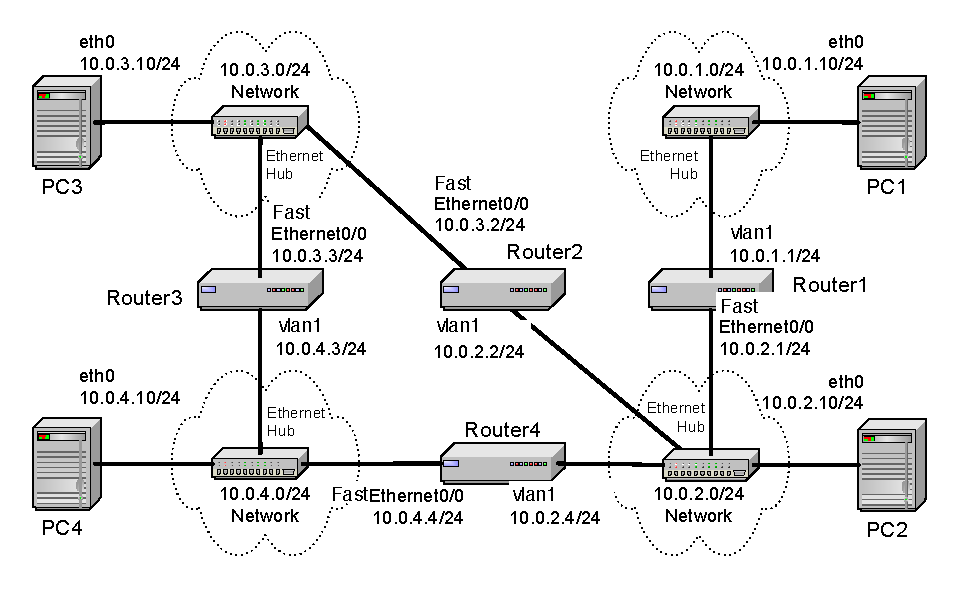
\includegraphics[width=\linewidth]{graphics/lab4-network1-part3-updated.pdf}	
	\caption{Network configuration for Part 3.}
	\label{fig:lab4-network1-part3}
\end{figure}

\begin{table}[h!t]
	\centering
	\begin{tabular}{| c | c | c |}	
		\hline
		\textbf{Cisco Router} & \textbf{FastEthernet0/0} & \textbf{vlan1} \\ \hline
		Router4 & 10.0.4.4/24 & 10.0.2.4/24 \\ \hline
	\end{tabular}
	\caption{IP addresses of Router4}
	\label{tab:lab4-network1-part3}
\end{table}

\subsubsection*{Exercise 3-A. Updating the routing tables}

Add Router4 to the network and observe the routing table updates made by RIP to reflect the new topology.

\begin{enumerate}
	\item Continue with the network configuration of Part 2. RIP must be enabled on all Routers shown in Figure \ref{fig:lab4-network1}, and a RIP process must be running (in passive mode) on all Linux PCs.
	\item Before attaching Router4, save the routing tables on all four Linux PCs with the command \cmd{netstat -rn}.
	\item Connect Router4 as shown in Figure \ref{fig:lab4-network1-part3} and assign the IP addresses to the interfaces as shown in Table \ref{tab:lab4-network1-part3}.
	\item Configure Router4 to run RIP, following the same steps as in Part 1.
	\item Use the command \cmd{netstat -rn} on the Linux PCs to observe how the routing tables are updated. Once the routing tables on the PCs have converged, save the routing tables on all four Linux PCs.
\end{enumerate}

\begin{questions}
	\q{3.A}{Include the routing tables of the Linux PCs before the topology was changed (Step 2) and after Router4 has been added and the routing tables have been updated (Step 5). Discuss the time it took to update the routing tables.}
\end{questions}

\subsubsection*{Exercise 3-B. Convergence of RIP after a link failure}

Next you disconnect the Ethernet cable of interface Ethernet0/0 on Router4 and observe how much time RIP takes to update the routing table of the Linux PCs to reflect the new topology.

\begin{enumerate}
	\item Issue a \cmd{ping} command from PC4 to PC1. Do not terminate the \cmd{ping} command until this exercise is completed in Step 4.
		\begin{cmdblock}
	PC4% ping 10.0.1.10
		\end{cmdblock}
	\item Disconnect the Ethernet cable connected to interface \iface{FastEthernet0/0} on Router4. Now, the output of ping on PC4 should show that the destination network is unreachable.
	\item Wait until the ping command is successful again, that is, ICMP Echo Reply messages arrive at PC4. This occurs once an alternate path has been found between PC4 and PC1, and the routing tables have been updated accordingly. This may take several minutes.
	\item Stop the ping command with \cmd{Ctrl-c} and save the ping statistics output (i.e. the data that appears at the bottom of the terminal screen when you stop the ping process).
	\item Count the number of lost packets and calculate the time it took RIP to update the routing tables. (The \cmd{ping} command issues an ICMP Echo Request message approximately once every second.)
\end{enumerate}

\begin{questions}
	\q{3.B}{Include your answer on the convergence time from Step 4. Count the number of lost packets and calculate the time it took RIP to update the routing tables. (The ping command issues an ICMP Echo Request message approximately once every second.)}
\end{questions}

\newpage
\subsection{Configuring Open Shortest Path First (OSPF)}

Next, you explore the routing protocol Open Shortest Path First (OSPF). OSPF is a link state routing protocol, where each router sends information on the cost metric of its network interfaces to all other routers in the network. The information about the interfaces is sent in messages that are called link state advertisements (LSAs). LSAs are disseminated using flooding, that is, a router sends its LSAs to all its neighbours, which, in turn, forward the LSAs to their neighbours, and so on. However, each LSA is forwarded only once. Each router maintains a link state database of all received LSAs, which provides the router with complete information about the topology of the network. Routers use their link state databases to run a shortest path algorithm that computes the shortest paths in the network.

Unlike distance vector routing protocols, link state routing protocols do not have convergence problems, such as the count-to-infinity problem. This is seen as a significant advantage of link state protocols over distance vector protocols.

OSPF is the most important link state routing protocol on the Internet. The functionality of OSPF is rich, and the lab exercises highlight only a small portion of the OSPF protocol. The Internet Lab uses OSPF version 2 (OSPFv2).
The network configuration is shown in Figure \ref{fig:lab4-network2} and Table \ref{tab:lab4-network2}. Note that some Linux PCs and routers are connected with crossover cables.

\begin{figure}[ht]
	\centering
	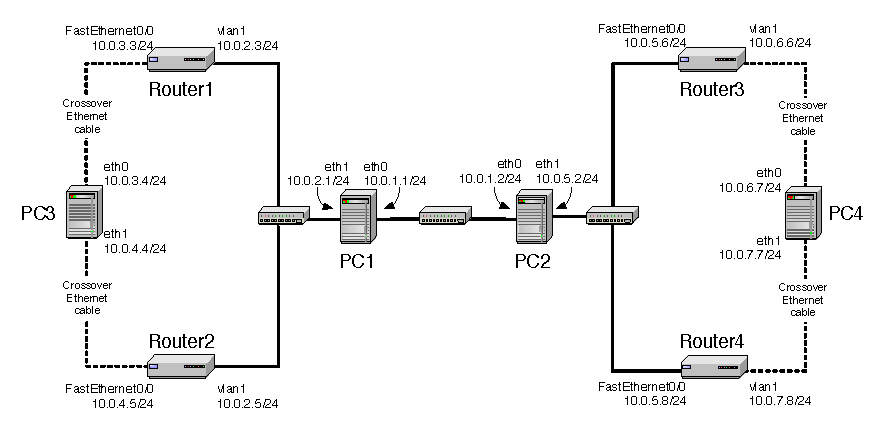
\includegraphics[width=\linewidth]{graphics/lab4-network2-updated.pdf}	
	\caption{Network configuration for Part 4.}
	\label{fig:lab4-network2}
\end{figure}

\begin{table}[h!t]
	\centering
	\begin{tabular}{| c | c | c |}	
		\hline
		\textbf{Linux PC} & \textbf{eth0} & \textbf{eth1} \\ \hline
		PC1 & 10.0.1.1/24 & 10.0.2.1/24 \\ 
		PC2 & 10.0.1.2/24 & 10.0.5.2/24 \\
		PC3 & 10.0.3.4/24 & 10.0.4.4/24 \\
		PC4 & 10.0.6.7/24 & 10.0.7.7/24 \\ \hline
		\textbf{Cisco Router} & \textbf{FastEthernet0/0} & \textbf{vlan1} \\ \hline
		Router1 & 10.0.3.3/24 & 10.0.2.3/24 \\
		Router2 & 10.0.4.5/24 & 10.0.2.5/24 \\
		Router3 & 10.0.5.6/24 & 10.0.6.6/24 \\
		Router4 & 10.0.5.8/24 & 10.0.7.8/24 \\ \hline
	\end{tabular}
	\caption{IP addresses for Part 5}
	\label{tab:lab4-network2}
\end{table}

\subsubsection*{Exercise 4-A. Configuring OSPF on Cisco routers}

Here, you configure OSPF on the Cisco routers. Below we give a brief description of the basic IOS commands used to configure OSPF on a Cisco router. As usual, each command must be issued in a particular IOS command mode.

\begin{enumerate}
	\item Connect the routers as shown in Figure \ref{fig:lab4-network2}. Some of the interfaces are connected with crossover cables or with hubs in between them.
	\item Configure the Cisco routers to run OSPF. The following set of commands are used to configure Router1.
		\begin{cmdblock}
	Router1> enable
	Password: <enable secret>
	Router1# configure terminal
	Router1(config)# no ip routing
	Router1(config)# ip routing
	Router1(config)# no router rip
	Router1(config)# router ospf 1
	Router1(config-router)# network 10.0.0.0 0.255.255.255 area 1 
	Router1(config-router)# interface FastEthernet0/0 
	Router1(config-if)# ip address 10.0.3.3 255.255.255.0 
	Router1(config-if)# interface vlan1
	Router1(config-if)# ip address 10.0.2.3 255.255.255.0
	Router1(config-if)# end 
	Router1# clear ip route *
		\end{cmdblock}
		The above commands disable RIP, enable OSPF for Area 1 and network 10.0.0.0/8, and configure the IP addresses of the routers. Since no router-id is specified, the highest IP address of Router1, 10.0.3.3, is used as the router-id. The router-id can be verified by issuing the command \cmd{show ip ospf}.
	\item Repeat the configuration on the other routers. Refer to Figure \ref{fig:lab4-network2} for the connections, and to Table \ref{fig:lab4-network2} for the IP addresses.
\end{enumerate}

\subsubsection*{Exercise 4-B. Configuring OSPF on Linux PCs}

On the Linux PCs, OSPF is configured using the Quagga package. The syntax of the Quagga commands is essentially identical to the corresponding IOS commands. All PCs are set up as IP routers. The following describes the configuration of PC1.
\begin{enumerate}
	\item Connect PC1 as shown in Figure \ref{fig:lab4-network2}.
	\item Enable IP forwarding on PC1 by typing
		\begin{cmdblock}
	PC1% echo "1" > /proc/sys/net/ipv4/ip_forward
		\end{cmdblock}
	\item Terminate the existing ripd process and disable the \cmd{ripd} daemon in the \path{daemons} configuration file: 
		\begin{cmdblock}
	PC1% /etc/init.d/quagga stop
		\end{cmdblock}
	\item Disabel the \cmd{ripd} and enable the \cmd{ospfd} daemon in the \path{daemons} configuration file: 
		\begin{cmdblock}
	zebra=yes
	bgpd=no
	ospfd=yes
	ospf6d=no
	ripd=no
	ripngd=no
	isisd=no
		\end{cmdblock}
	\item Restart Quagga
		\begin{cmdblock}
	PC1% /etc/init.d/quagga start
		\end{cmdblock}
	\item Set the OSPF configuration on PC1. Note that the commands for configuring OSPF in Quagga are very similar to the IOS commands:
		\begin{cmdblock}
	PC1% telnet localhost 2604 Password: <login password>
	ospfd> enable
	ospfd# configure terminal
	ospfd(config)# router ospf 
	ospfd(config-router)# network 10.0.0.0/8 area 1 
	ospfd(config-router)# router-id 10.0.1.1 
	ospfd(config-router)# no passive-interface eth0 
	ospfd(config-router)# no passive-interface eth1
	ospfd(config-router)# end
	ospfd# exit
		\end{cmdblock}
		Note that the command to enable OSPF (\cmd{router ospf}) does not use a process-id. Also, there is an explicit command to set the router-id. The latter is necessary since Quagga does not assign a default value for the router-id. In Quagga, the router-id must be explicitly set. In this exercise we use the IP address of the Ethernet interface \iface{eth0} as the router-id for the Linux PCs.
	\item Repeat the OSPF configuration in Steps 1-6 for all other Linux PCs.
	\item When the OSPF configuration is complete, all hosts and routers should be able to communicate with each other. You can test the network configuration by running \cmd{traceroute} and \cmd{ping} commands on a Linux PC (or trace and ping commands on a Cisco router). When you have verified that the network connection is correct, proceed with the next step.
\end{enumerate}

\subsubsection*{Exercise 4-C. Observing Convergence of OSPF}

In comparison to the distance vector protocol RIP, the link state routing protocol OSPF quickly adapts to changes in the network topology. In this exercise you observe the interactions of OSPF after a change to the network topology.
\begin{enumerate}
	\item On PC1, start to capture traffic with Wireshark on interface \iface{eth0}. Set a filter to only display OSPF packets.
	\item From PC3, run a \cmd{traceroute} command to PC4 
		\begin{cmdblock}
	PC3% traceroute 10.0.7.7
		\end{cmdblock}
		Confirm from the output and Figure \ref{fig:lab4-network2}, whether the path from PC3 to PC4 includes Router 3 or Router4.
	\item Issue a \cmd{ping} command from PC3 to PC4 (10.0.7.7). Do not terminate the \cmd{ping} command until this exercise is completed.
		\begin{cmdblock}
	PC3% ping 10.0.7.7
		\end{cmdblock}
	\item If the path from PC3 to IP address 10.0.7.7 from Step 2 included Router3, then disconnect the Ethernet cable of the \iface{Ethernet0/1} interface of Router3. Otherwise, disconnect the Ethernet cable of the \iface{Ethernet0/1} interface of Router4.
When the Ethernet cable is disconnected, the \cmd{ping} command on PC3 will show that IP address 10.0.7.7 is not reachable.
	\item Now, OSPF updates the routing tables. Use the Wireshark window on PC1 to observe the transmitted OSPF messages:
\end{enumerate}

\begin{questions}
	\q{4.C.1.a}{How quickly are OSPF messages sent after the cable is disconnected?}
	\q{4.C.1.b}{How many OSPF messages are sent?}
	\q{4.C.1.c}{Which type of OSPF packet is used for flooding link state information?}
	\q{4.C.1.d}{Describe the flooding of LSAs to all routers.}
	\q{4.C.1.e}{Which type of encapsulation is used for OSPF packets (TCP, UDP or other)?}
	\q{4.C.1.f}{What is the destination address of OSPF packets?}
\end{questions}

\begin{enumerate}[resume]
	\item Wait until the \cmd{ping} command is successful again, that is, ICMP Echo Reply messages arrive at PC3. This happens when the routing tables have been updated.
	\item Stop the ping command with \cmd{Ctrl-c} and save the ping statistics output (i.e. the data that appears at the bottom of the terminal screen when you stop the ping process).
\end{enumerate}

\begin{questions}
	\q{4.C.2}{Include your answer on the convergence time from Step 7. Count the number of lost packets and calculate the time it took OSPF to update the routing tables. (The ping command issues an ICMP Echo Request message approximately once every second.)}
\end{questions}

\begin{enumerate}[resume]
	\item Issue another \cmd{traceroute} command from PC3 to IP address 10.0.7.7. By now, the output should show the new route to PC4.
	\item Save the link state database on all Cisco routers and on all Linux PCs, and verify that all routers indeed have the same link state database. On the Linux PCs, open a Telnet session to the ospfd process, and then type
		\begin{cmdblock}
	ospfd# show ip ospf database router
		\end{cmdblock}
		On the Cisco routers, simply type
		\begin{cmdblock}
	Router1# show ip ospf database
		\end{cmdblock}
		Save the output of the link state databases to a file.
\end{enumerate}

\begin{questions}
	\q{4.C.3}{ Can you confirm that the link state databases are identical? Compare the output of the command \cmd{show ip ospf database} from the Cisco routers and the Linux PCs.}
\end{questions}

\begin{enumerate}[resume]
	\item Stop Wireshark on PC1, and save the different types of OSPF packets captured by Wireshark. Save one copy of each type of OSPF packet that you observed (Selecting the Print Detail option).
\end{enumerate}

\begin{questions}
	\q{4.C.4}{From your saved Wireshark output, include one packet from each of the different OSPF packet types that you have observed. (Include only one packet from each type!)}
	\q{4.C.5}{Include the output of the link state database of PC2.}
	\q{4.C.6}{Pick a single link state advertisement packet captured by Wireshark, and describe how to interpret the information contained in the link state advertisement.}
\end{questions}

\newpage
\subsection{Hierarchical Routing in OSPF}

The concept of areas in OSPF can be used to construct a hierarchical routing scheme. When the network is partitioned into multiple areas, then routers must have complete topology information only about routers in the same area, and only limited information about other areas. All areas must be connected to Area 0, which is a special area, called the backbone area. This builds a two-level hierarchy: The backbone area is at the top of the hierarchy and the other areas are at the bottom of the hierarchy. Traffic between two areas is routed through the backbone area. Routers that connect to two areas are called area border routers.

The configuration in this part is shown in Figure \ref{fig:lab4-network2-part5}. Here, the network from Part 4 is partitioned into three areas. The area in the middle is the backbone area (Area 0). The IP addresses are the same as in Part 4, and need not be modified. PC1 and PC2 are area border routers.

\begin{figure}[h!t]
	\centering
	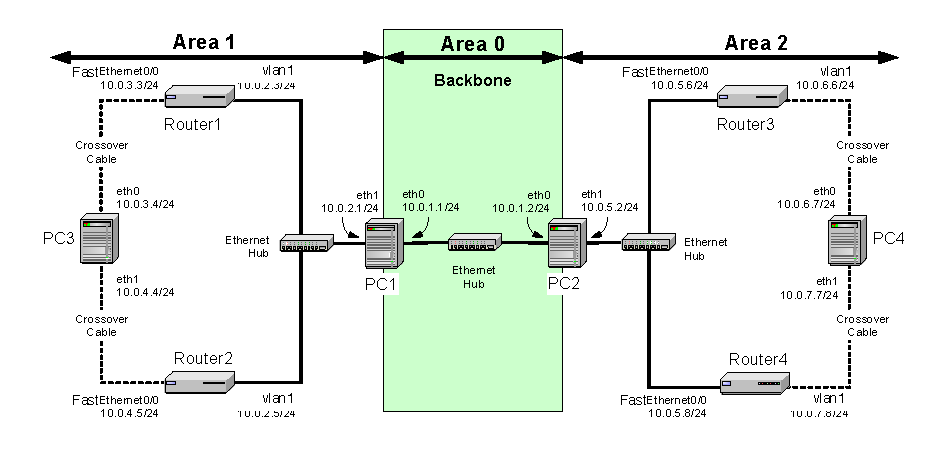
\includegraphics[width=\linewidth]{graphics/lab4-network2-part5-updated.pdf}	
	\caption{Network configuration for Part 5}
	\label{fig:lab4-network2-part5}
\end{figure}

In the following exercises you define the areas, and then observe how the link state databases are built.

\subsubsection*{Exercise 5. Defining multiple areas in OSPF}

\begin{enumerate}
	\item Restart the \cmd{zebra} and \cmd{ospfd} processes on all four Linux PCs. Use the same \path{daemons} configuration file as used in the previous exercise.
		\begin{cmdblock}
	PC1% /etc/init.d/quagga restart
		\end{cmdblock}
	\item Start Wireshark on PC1 and capture traffic on interface \iface{eth0}.
	\item Change the Area IDs of the Cisco routers and the PCs. On each system, the directly connected networks are assigned to an area with a 24-bit prefix. Here are the configurations for PC3, PC1, and Router 1. The other configurations are similar.
		PC3, which belongs to only one area, is configured as follows:
		\begin{cmdblock}
	PC3% telnet localhost 2604 Password: <login password>
	ospfd> enable
	ospfd# configure terminal
	ospfd(config)# router ospf 
	ospfd(config-router)# router-id 10.0.3.4 
	ospfd(config-router)# network 10.0.3.0/24 area 1 
	ospfd(config-router)# network 10.0.4.0/24 area 1 
	ospfd(config-router)# end
	ospfd# exit
		\end{cmdblock}
		PC1, belongs to two areas, and is configured as follows:
		\begin{cmdblock}
	PC1% telnet localhost 2604 Password: <login password>
	ospfd> enable
	ospfd# configure terminal
	ospfd(config)# router ospf 
	ospfd(config-router)# router-id 10.0.1.1 
	ospfd(config-router)# network 10.0.2.0/24 area 1 
	ospfd(config-router)# network 10.0.1.0/24 area 0 
	ospfd(config-router)# end
	ospfd# exit
		\end{cmdblock}
		The configuration of Router 1 is as follows:
		\begin{cmdblock}
	Router1# configure terminal
	Router1(config)# no router ospf 1
	Router1(config)# router ospf 1
	Router1(config-router)# network 10.0.3.0 0.0.0.255 area 1
	Router1(config-router)# network 10.0.2.0 0.0.0.255 area 1 
	Router1(config-router)# end
	Router1# clear ip ospf 1 process
		\end{cmdblock}
	\item Once the routing tables have converged, test the network configuration with the commands \cmd{traceroute} and \cmd{ping} on the Linux PCs, and the commands trace and ping on the Cisco routers. All hosts and routers should be able to communicate with each other.
	\item Save the link state database on all Cisco routers and on all Linux PCs. On the Linux PCs, open a Telnet session to the ospfd process, and then type
		\begin{cmdblock}
	ospfd# show ip ospf database router
		\end{cmdblock}
		On the Cisco routers, type
		\begin{cmdblock}
	Router1# show ip ospf database
		\end{cmdblock}
		Save the output of the link state databases to a file.
\end{enumerate}

\begin{questions}
	\q{5.1.a}{Refer to the saved link state databases in your answers. Compare the link state databases to those saved in Part 4. Which differences do you note?}
	\q{5.1.b}{Which information do routers in Area 1 have about Area 2? Which information do they have about the backbone area (Area 0)?}
	\q{5.1.c}{How much information do the routers in the backbone area (Area 0) have about the topology of Area 1 and Area 2?}
	\q{5.1.d}{How do the IP routers in Area 1 know how to forward traffic to Area 2?}
\end{questions}

\begin{enumerate}[resume]
	\item Display the area routers known to Router 1 from Area 1, with the command
		\begin{cmdblock}
	Router1# show ip ospf border-routers
		\end{cmdblock}
		Save the output to a file.
	\item Save the Wireshark output of OSPF packet types (selecting the Print Detail option) that you did not observe in Part 4. Only include one packet of each type.
\end{enumerate}

\begin{questions}
	\q{5.2}{Include the Wireshark output in your report showing, if any, the different types of OSPF packets that you did not observe in Part 5.}
	\q{5.3}{Include the output of the link state databases saved in Step 5.}
	\q{5.4}{Explain the output of the command ``show ip ospf border-routers'' in Step 6.}
\end{questions}

\setcounter {chapter} {4}
%%!TEX root = labo.tex

\chapter{Transport Layer Protocols: UDP and TCP}

What you will learn in this lab:
\begin{itemize}
	\item The differences between data transfers with UDP and with TCP
	\item What effect IP Fragmentation has on TCP and UDP
	\item How to analyze measurements of a TCP connection
	\item The difference between interactive and bulk data transfers in TCP
	\item How TCP performs retransmissions
	\item How TCP congestion control works
\end{itemize}

\newpage
\setsession{prelab5}
\section{Prelab 5}\label{sec:prelab5}
%!TEX root = labo.tex

\subsubsection*{TCP and UDP}
Use the following resources to prepare yourself for this lab session:
\begin{enumerate}
	\item TCP and UDP: Read the overview of TCP and UDP available at \url{http://en.wikipedia.org/wiki/Transmission_Control_Protocol} and \url{http://en.wikipedia.org/wiki/User_Datagram_Protocol}.
	\item IP Fragmentation: Refer to the website \\ \url{http://www.tcpipguide.com/free/t_IPMessageFragmentationProcess.htm} for information on IP Fragmentation and Path MTU Discovery.
	\item TCP Retransmissions: Refer to RFC 2988, which is available at \url{http://tools.ietf.org/html/rfc2988},
and read about TCP retransmissions.
	\item TCP Congestion Control: Refer RFC 2001, which is available at \url{http://tools.ietf.org/html/rfc2001},
and read about TCP congestion control.
\end{enumerate}

\newpage
\subsection*{Prelab Questions}
\begin{questions}
	\q{1}{Explain the role of port numbers in TCP and UDP.}
	\q{2}{Provide the syntax of the \cmd{ttcp} command for both the sender and receiver, which executes the following scenario: A TCP server has IP address 10.0.2.6 and a TCP client has IP address 10.0.2.7. The TCP server is waiting on port number 2222 for a connection request. The client connects to the server and transmits 2000 bytes to the server, which are sent as 4 write operations of 500 bytes each.}
	\q{3.a}{How does TCP decide the maximum size of a TCP segment?}
	\q{3.b}{How does UDP decide the maximum size of a UDP datagram?}
	\q{3.c}{What is the ICMP error generated by a router when it needs to fragment a datagram with the DF bit set? Is the MTU of the interface that caused the fragmentation also returned?}
	\q{3.d}{Explain why a TCP connection over an Ethernet segment never runs into problems with fragmentation.}
	\q{4}{Assume a TCP sender receives an acknowledgement (ACK), that is, a TCP segment with the ACK flag set, where the acknowledgement number is set to 34567 and the window size is set to 2048. Which sequence numbers can the sender transmit?}
	\q{5.a}{Describe Nagle's algorithm and explain why it is used in TCP}
	\q{5.b}{Describe Karn's Algorithm and explain why it is used in TCP}
	\q{6.a}{What is a delayed acknowledgement in TCP?}
	\q{6.b}{What is a piggybacked acknowledgement in TCP?}
	\q{7}{Describe how the retransmission timeout (RTO) value is determined in TCP.}
	\q{8.a}{Describe the sliding window flow control mechanism used in TCP .}
	\q{8.b}{Describe the concepts of slow start and congestion avoidance in TCP.}
	\q{8.c}{Explain the concept of fast retransmit and fast recovery in TCP.}
\end{questions}


\newpage
\setsession{lab5}
\section{Lab 5}\label{sec:lab5}

This lab explores the operation of the Transmission Control Protocol (TCP) and the User Datagram Protocol (UDP), the two transport protocols of the Internet protocol architecture.

UDP is a simple protocol for exchanging messages from a sending application to a receiving application. UDP adds a small header to the message, and the resulting data unit is called a UDP datagram. When a UDP datagram is transmitted, the datagram is encapsulated in an IP header and delivered to its destination. There is one UDP datagram for each application message.

The operation of TCP is more complex. First, TCP is a connection-oriented protocol, where a TCP client establishes a logical connection to a TCP server, before data transmission can take place. Once a connection is established, data transfer can proceed in both directions. The data unit of TCP, called a TCP segment, consists of a TCP header and payload which contains application data. A sending application submits data to TCP as a single stream of bytes without indicating message boundaries in the byte stream. The TCP sender decides how many bytes are put into a segment.

TCP ensures reliable delivery of data, and uses checksums, sequence numbers, acknowledgements, and timers to detect damaged or lost segments. The TCP receiver acknowledges the receipt of data by sending an acknowledgement segment (ACK). Multiple TCP segments can be acknowledged in a single ACK. When a TCP sender does not receive an ACK, the data is assumed lost, and is retransmitted.

TCP has two mechanisms that control the amount of data that a TCP sender can transmit. First, TCP receiver informs the TCP sender how much data the TCP sender can transmit. This is called flow control. Second, when the network is overloaded and TCP segments are lost, the TCP sender reduces the rate at which it transmits traffic. This is called congestion control.

The lab covers the main features of UDP and TCP. Parts 1 and 2 compare the performance of data transmissions in TCP and UDP. Part 3 explores how TCP and UDP deal with IP fragmentation. The remaining parts address important components of TCP. Part 4 explores connection management, Parts 5 and 6 look at flow control and acknowledgements, Part 7 explores retransmissions, and Part 8 is devoted to congestion control.

This lab has two different network topologies. The topology for Parts 1-4 is shown in Figure \ref{fig:lab5-network-topology1}. In this configuration, PC1 and PC2 are used as hosts, and PC3 is set up as an IP router. The network configuration for Parts 5-8 is shown in Figure \ref{fig:lab5-network-topology2}. Here, the four Cisco routers interconnected via Ethernet, where one of the links is configured to emulate a slow serial link, as show in Figure \ref{fig:lab5-network-topology2}.

\newpage
\subsection{Learning how to use nttcp}

The \cmd{nttcp} command is a Linux tool used to generate synthetic UDP and TCP traffic loads. Together with \cmd{ping} and \cmd{traceroute}, \cmd{nttcp} is an essential utility program for debugging problems in IP networks. Running \cmd{nttcp} tool consists of setting up a nttcp receiver on one hosts and then a nttcp sender on another host. Once the nttcp sender is started, it blasts the specified amount of data as fast as possible to the nttcp receiver.

\boxinfo{Some useful \cmd{nttcp} commands:
	\begin{description}
		\item[\texttt{nttcp -u -i -rs -lbuflen -nnumbufs -pport}]\hfill \\
			Start a nttcp receiver process
		\item[\texttt{nttcp -u -ts -lbuflen -nnumbufs -pport -D IPaddress}]\hfill \\
			Start a nttcp sender process
	\end{description}
}

\boxinfo{List of important \cmd{nttcp} options:
	\begin{description}
		\item[\texttt{-t}]\hfill \\
			Specifies the transmit mode.
		\item[\texttt{-r}]\hfill \\
			Specifies the receive mode
		\item[\texttt{-u}]\hfill \\
			Specifies to use UDP instead of TCP. By default, nttcp uses TCP to send data. Make sure this is the first option
		\item[\texttt{-s}]\hfill \\
			Sends a character string as payload of the transmitted packets. Without the -s option, the default is to transmit data from the terminal window (stdin) of the sender and to print the received data to the terminal window (stdout) at the receiver
		\item[\texttt{-nnumbufs}]\hfill \\
			Number of blocks of application data to be transmitted (Default value is 2048)
		\item[\texttt{-lbuflen}]\hfill \\
			Length of the application data blocks that are passed to UDP or TCP in bytes (default 8192). When UDP is used, this value is the number of data bytes in UDP datagram
		\item[\texttt{-D}]\hfill \\
			Disables buffering of data in TCP and forces immediate transmission of the data at the nttcp sender. Only used in the context of TCP
		\item[\texttt{-pport}]\hfill \\
			Port number to send to or listen on. The port number must be identical at the sender and at the receiver. The default value is 5000
		\item[\texttt{IPaddress}]\hfill \\
			IP address of the nttcp receiver
	\end{description}
}

By default, nttcp transmits data over a TCP connection. The nttcp sender opens a TCP connection to a nttcp receiver, transmits data and then closes the connection. The nttcp receiver must be running when the nttcp sender is started. UDP data transfer is specified with the \cmd{-u} option. Since UDP is a connectionless protocol, the nttcp sender starts immediately sending UDP datagrams, regardless if there is a nttcp receiver established or not.

\begin{figure}[ht]
	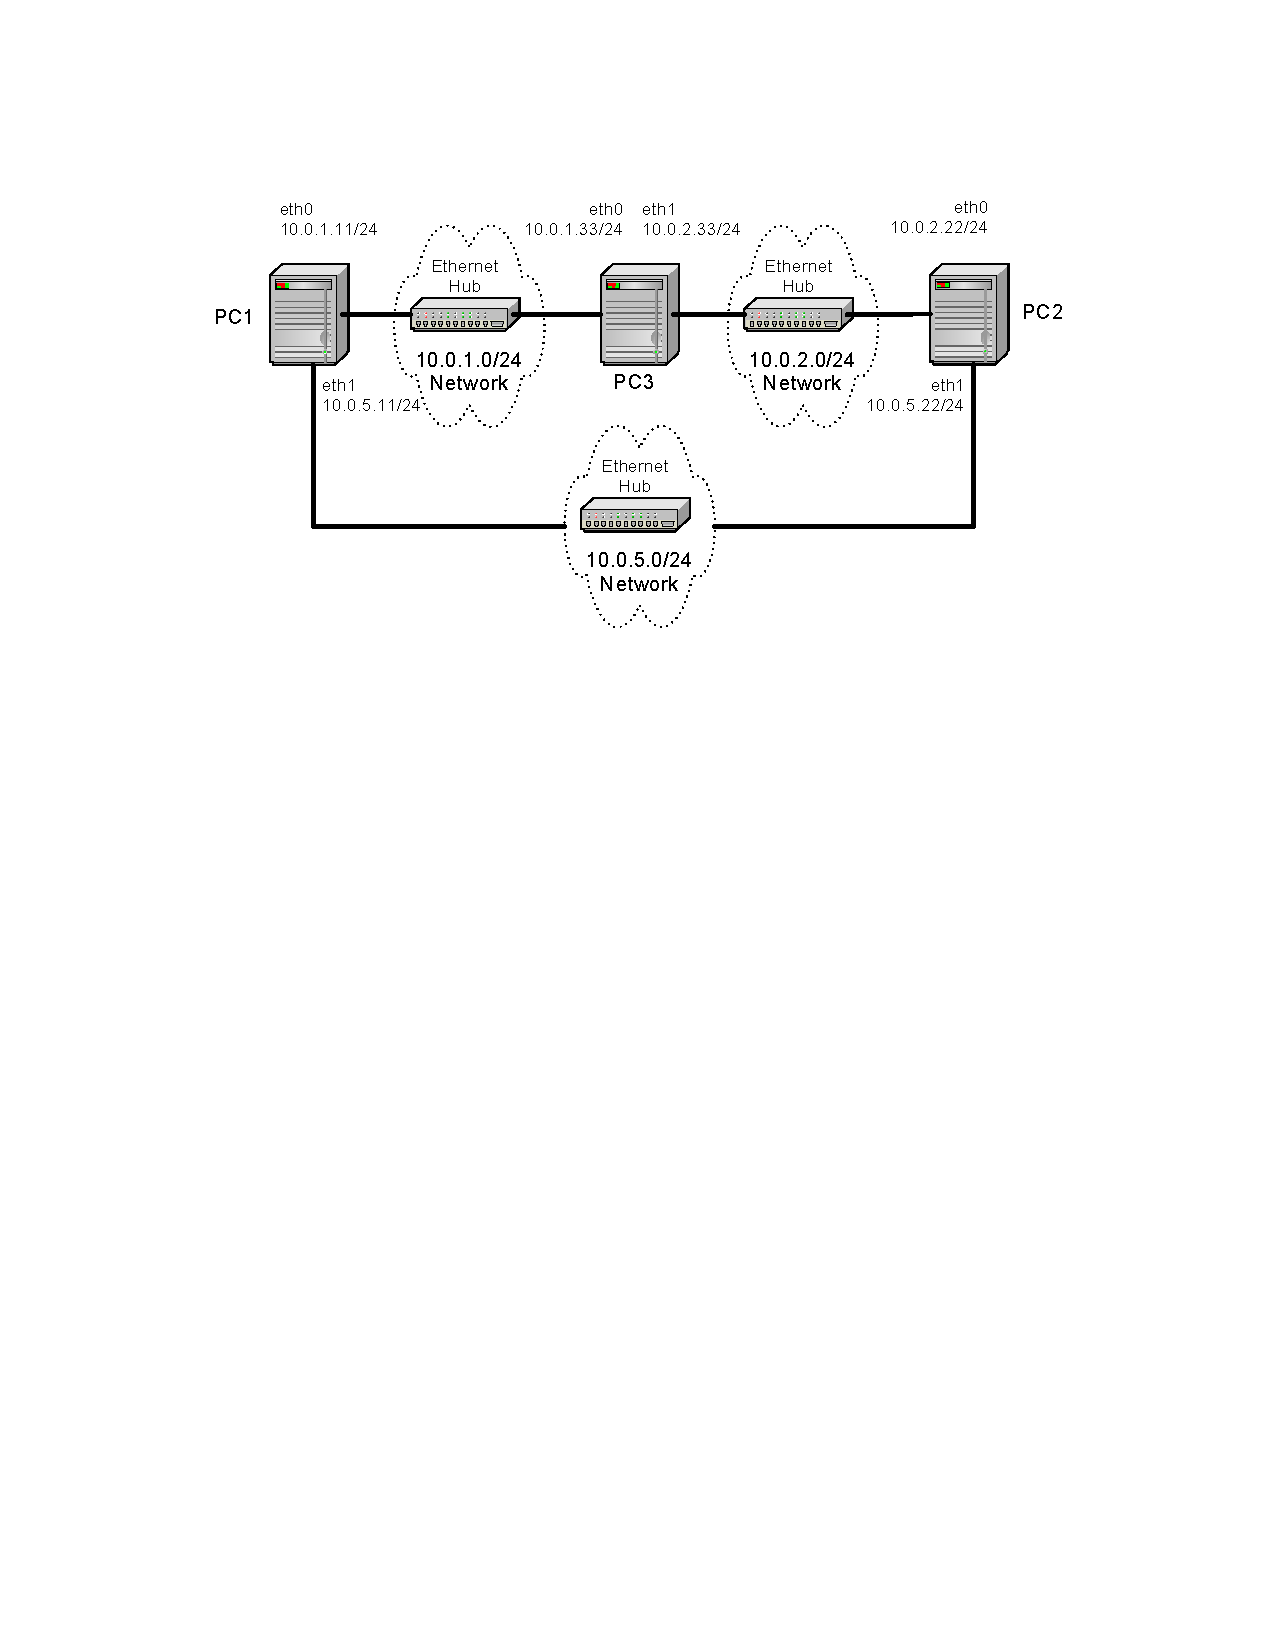
\includegraphics{graphics/fig-5-1.pdf}	
	\caption{Network Topology for Parts 1-4.}
	\label{fig:lab5-network-topology1}
\end{figure}

\begin{table}[ht]
	\centering
	\begin{tabular}{| c | c | c |}	
		\hline
		\textbf{Linux PC} & \textbf{Ethernet Interface eth0} & \textbf{Ethernet Interface eth1}  \\ \hline
		PC1 & 10.0.1.11/24 & 10.0.5.11/24 \\ 
		PC2 & 10.0.2.22/24 & 10.0.5.22/24 \\
		PC3 & 10.0.1.33/24 & 10.0.2.33/24 \\ \hline
	\end{tabular}
	\caption{IP Addresses of the Linux PCs.}
	\label{tab:lab5-ip-addresses}
\end{table}


\subsubsection{Exercise 1-a. Network setup}
\begin{enumerate}
	\item Connect the Ethernet interfaces of the Linux PCs as shown in Figure \ref{fig:lab5-network-topology1}. Configure the IP addresses of the interfaces as given in Table \ref{tab:lab5-ip-addresses}.
	\item PC1 and PC2 are set up as hosts and IP forwarding should be disabled. On PC1, this is done with the command
		\begin{cmdblock}
	PC1% echo "0" > /proc/sys/net/ipv4/ip_forward
		\end{cmdblock}
	\item PC3 is set up as an IP router. Enable IP forwarding on PC3 with the command
		\begin{cmdblock}
	PC3% echo "1" > /proc/sys/net/ipv4/ip_forward
		\end{cmdblock}
	\item Add default routes to the routing tables of PC1 and PC2, so that PC3 is the default gateway. For PC1 the command is as follows:
		\begin{cmdblock}
	PC1% route add default gw 10.0.1.33
		\end{cmdblock}
	\item Verify that the setup is correct by issuing a \cmd{ping} command from PC1 to PC2 over both paths:
		\begin{cmdblock}
	PC1% ping 10.0.2.22 
	PC1% ping 10.0.5.22
		\end{cmdblock}
\end{enumerate}

\subsubsection{Exercise 1-b. Transmitting data with UDP}

This exercise consists of setting up a UDP data transfer between two hosts, PC1 and PC2, and observe the UDP traffic.

\begin{enumerate}
	\item On PC1, start Wireshark to capture packets on interface \iface{eth1} between PC1 to PC2. 
		\begin{cmdblock}
	PC1% wireshark -i eth1 -f 'host 10.0.5.22'
		\end{cmdblock}
		This sets a capture filter to packets that include IP address 10.0.5.22 in the IP header. Start to capture traffic.
	\item On PC2, start a nttcp receiver that receives UDP traffic with the following command: 
		\begin{cmdblock}
			PC2% nttcp -u -i -rs -l1024 -n10 -p4444
		\end{cmdblock}
	\item On PC1, start a nttcp sender that transmits UDP traffic by typing: 
		\begin{cmdblock}
			PC1% nttcp -u -ts -l1024 -n10 -p4444 10.0.5.22
		\end{cmdblock}
		Observe the captured traffic captured by Wireshark. 
	\item Stop the Wireshark capture on PC1 and save the captured traffic.
\end{enumerate}

\textbf{Use the data captured with Wireshark to answer the questions in Step 3. Support your answers with the saved Wireshark data.}
\begin{questions}
	\q{1.B.1.a}{How many packets are exchanged in the data transfer? How many packets are transmitted for each UDP datagram? What is the size of the UDP payload of these packets?}
	\q{1.B.1.b}{Compare the total number of bytes transmitted, in both directions, including Ethernet, IP, and UDP headers, to the amount of application data transmitted.}
	\q{1.B.1.c}{Inspect the fields in the UDP headers. Which fields in the headers do not change in different packets?}
	\q{1.B.1.d}{Observe the port numbers in the UDP header. How did the nttcp sender select the source port number?}
\end{questions}

\subsubsection{Exercise 1-c. Transmitting data with TCP}

Here, you repeat the previous exercise, but use TCP for data transfer.
\begin{enumerate}
	\item On PC1, start Wireshark and capture packets on interface \iface{eth1} between PC1 to PC2:
		\begin{cmdblock}
	PC1% wireshark -i eth1 -f 'host 10.0.5.22'
		\end{cmdblock}
	\item Start a nttcp receiver on PC2 that receives packets sent by PC1: 
		\begin{cmdblock}
	PC2% nttcp -i -rs -l1024 -n10 -p4444
		\end{cmdblock}
	\item Start a nttcp sender on PC1o that transmits packets from PC1 to PC2: 
		\begin{cmdblock}
	PC1% nttcp -ts -l1024 -n10 -p4444 -D 10.0.5.22
		\end{cmdblock}
\end{enumerate}

\textbf{Use the data captured with Wireshark to answer the questions in Step 3. Support your answers by including data from the saved Wireshark data captures.}
\begin{questions}
	\q{1.C.1.a}{How many packets are exchanged in the data transfer? What are the sizes of the TCP segments?}
	\q{1.C.1.b}{What is the range of the sequence numbers?}
	\q{1.C.1.c}{How many packets are transmitted by PC1 and how many packets are transmitted by PC2?}
	\q{1.C.1.d}{How many packets do not carry a payload, that is, how many packets are control packets?}
	\q{1.C.1.e}{Compare the total number of bytes transmitted, in both directions, including Ethernet, IP, and UDP headers, to the amount of application data transmitted.}
	\q{1.C.1.f}{Inspect the TCP headers. Which packets contain flags in the TCP header? Which types of flags do you observe?}
\end{questions}

\begin{enumerate}[resume]
	\item Stop the wireshark capture on PC1, and save the captured traffic to files. Save both the summary and detail output in the Print menu.
\end{enumerate}

\begin{questions}
	\q{1.C.2}{Compare the amount of data transmitted in the TCP and the UDP data transfers.}
	\q{1.C.3}{Take the biggest UDP datagram and the biggest TCP segment that you observed, and compare the amount of application data that is transmitted in the UDP datagram and the TCP segment.}
\end{questions}
	
\newpage
\subsection{File Transfers using TCP and UDP}

Here you compare the throughput of a file transfer with TCP and UDP, using the application programs \cmd{ftp} and \cmd{tftp}.

The File Transfer Protocol (FTP) for copying files between hosts, as described in the Introduction, employs TCP as its transport protocol, thereby ensuring a reliable transfer of transmitted data. Two TCP connections are established for each FTP session: A control connection for exchanging commands, and a data connection for the file transfer.

The Trivial File Transfer Protocol (TFTP) is a minimal protocol for transferring files without authentication. TFTP employs UDP for data transport. A TFTP session is initiated when a TFTP client sends a request to upload or download a file to UDP port 69 of a TFTP server. When the request is received, the TFTP server picks a free UDP port and uses this port to communicate with the TFTP client. Since UDP does not recover lost or corrupted data, TFTP is responsible for maintaining the integrity of the data exchange. TFTP transfers data in blocks of 512 bytes. A block must be acknowledged before the next block can be sent. When an acknowledgment is not received before a timer expires, the block is retransmitted.

The purpose of the following exercises is to observe that, despite the overhead of maintaining a TCP connection, file transfers with FTP generally outperform those with UDP.

\subsubsection{Exercise 2. Comparison of FTP and TFTP}
Study the performance of FTP and TFTP file transfers for a large file.

\begin{enumerate}
	\item Create a large file. On PC1, create a file with name \path{large.d} in directory \path{/tftpboot} by using the \cmd{dd} tool. Create the file and change its access permissions as follows:
		\begin{cmdblock}
	PC1% dd if=/dev/urandom of=/tftpboot/large.d bs=1024 count=1024  
	PC1% chmod 644 /tftpboot/large.d
		\end{cmdblock}
		Use the command \cmd{ls -l} to check the length of the file.
	\item Start Wireshark: Invoke Wireshark on interface \iface{eth1} of PC1 with a capture filter set for PC2, and start to capture traffic:
		\begin{cmdblock}
	PC1% wireshark -i eth1 -f “host 10.0.5.22”
		\end{cmdblock}
	\item FTP file transfer: On PC2, perform the following steps:
		\begin{itemize}
			\item Change the current directory to \path{/labdata}.
			\item Start the FTP server on PC1 by typing
				\begin{cmdblock}
	PC1% service vsftpd start
				\end{cmdblock}
			\item Invoke an FTP session to PC1 by typing
				\begin{cmdblock}
	PC2% ftp 10.0.5.11
				\end{cmdblock}
				Log in as the root user.
			\item Transfer the file large.d from PC1 to directory \path{/labdata} on PC2 by typing
				\begin{cmdblock}
	ftp> cd /tftpboot 
	ftp> get large.d 
	ftp> quit
				\end{cmdblock}
		\end{itemize}
	\item TFTP file transfer: On PC2 perform the following tasks:
		\begin{itemize}
			\item Start the TFTP server on PC1 by typing
				\begin{cmdblock}
	PC1% service tftpd-hpa start
				\end{cmdblock}
			\item Start a TFTP session to PC1 by typing 
				\begin{cmdblock}
	PC2% tftp 10.0.5.11
				\end{cmdblock}
			\item Transfer the file \path{large.d} from PC1 to PC2. 
				\begin{cmdblock}
	tftp> get large.d
	tftp> quit
				\end{cmdblock}
				By default, TFTP copies data from the directory \path{/tftpboot}.
			\item Observe the output of the TFTP session and save the output to a file.
		\end{itemize}
	\item Analysis of outcome: On PC1, stop the Wireshark output.
\end{enumerate}

Include the answers to the questions in Step 5.
\begin{questions}
	\q{2.A.a}{From the timestamps recorded by wireshark, obtain the times it took to transfer the file with FTP and with TFTP? Use your knowledge of FTP, TFTP, TCP, and UDP to explain the outcome.}
	\q{2.A.b}{Identify the TCP connections that are created in the FTP session, and record the port numbers at the source and at the destination.}
\end{questions}

\newpage
\subsection{IP Fragmentation of UDP and TCP traffic}

In this part of the lab, you observe the effect of IP Fragmentation on UDP and TCP traffic. Fragmentation occurs when the transport layer sends a packet of data to the IP layer that exceeds the Maximum Transmission Unit (MTU) of the underlying data link network. For example, in Ethernet networks, the MTU is 1500 bytes. If an IP datagram exceeds the MTU size, the IP datagram is fragmented into multiple IP datagrams, or, if the Don’t fragment (DF) flag is set in the IP header, the IP datagram is discarded.

When an IP datagram is fragmented, its payload is split into multiple IP datagrams, each satisfying the limit imposed by the MTU. Each fragment is an independent IP datagram, and is routed in the network independently from the other fragments. Fragmentation can occur at the sending host or at intermediate IP routers. Fragments are reassembled only at the destination host.

Even though IP fragmentation provides flexibility that can hide differences of data link technologies to higher layers, it incurs considerable overhead, and, therefore, should be avoided. TCP tries to avoid fragmentation with an Path MTU Discovery scheme that determines a Maximum Segment Size (MSS) which does not result in fragmentation.

You explore the issues with IP fragmentation of TCP and UDP transmissions in the network configuration shown in Figure \ref{fig:lab5-network-topology1}, with PC1 as sending host, PC2 as receiving host, and PC3 as intermediate IP router.

\subsubsection{Exercise 3-a. UDP and Fragmentation}

In this exercise you observe IP fragmentation of UDP traffic. In the following exercise, use \cmd{nttcp} to generate UDP traffic between PC1 and PC2, across IP router PC3, and gradually increase the size of UDP datagrams until fragmentation occurs. You can observe that IP headers do not set the DF bit for UDP payloads.

\begin{enumerate}
	\item Verify that the network is configured as shown in Figure \ref{fig:lab5-network-topology1} and Table \ref{tab:lab5-ip-addresses}. The PCs should be configured as described in Exercise 1-a.
	\item Start Wireshark on the \iface{eth0} interfaces of both PC1 and PC2, and start to capture traffic. Do not set any filters.
	\item Use \cmd{nttcp} to generate UDP traffic between PC1 and PC2. The connection parameters are selected so that IP Fragmentation does not occur initially.
		\begin{itemize}
			\item On PC2, execute the following command:
				\begin{cmdblock}
	PC2% nttcp -u -i -rs -l1024 -n12 -p4444
				\end{cmdblock}
			\item On PC1, execute the command:
				\begin{cmdblock}
	PC1% nttcp -u -ts -l1024 -n12 -p4444 10.0.2.22
				\end{cmdblock}
		\end{itemize}
	\item Increment the size of the UDP datagrams, by increasing the argument given with the \cmd{-l} option.
		\begin{itemize}
			\item Determine the exact UDP datagram size at which fragmentation occurs.
			\item Determine the maximum size of the UDP datagram that the system can send and receive, regardless of fragmentation, i.e., fragmentation of data segments occurs until a point beyond which the segment size is too large for to be handled by IP.
		\end{itemize}
	\item Stop the traffic capture on PC1 and PC2, and save the Wireshark output.
\end{enumerate}

\begin{questions}
	\q{3.A.1}{From the saved Wireshark data, select one IP datagram that is fragmented. Include the complete datagram before fragmentation and include all fragments after fragmentation. For each fragment of this datagram, determine the values of the fields in the IP header that are used for fragmentation (Identification, Fragment Offset, Don’t Fragment Bit, More Fragments Bit).}
	\q{3.A.2}{Include the outcome of the experiment in Step 4. Indicate the UDP datagram size at which fragmentation occurs. Also, determine the maximum size of the UDP datagram that the system can send.}
\end{questions}

\subsubsection{Exercise 3-b. TCP and Fragmentation}

TCP tries to completely avoid fragmentation with the following two mechanisms:

\begin{itemize}
	\item When a TCP connection is established, it negotiates the maximum segment size (MSS). Both the TCP client and the TCP server send the MSS in an option that is attached to the TCP header of the first transmitted TCP segment. Each side sets the MSS so that no fragmentation occurs at the outgoing network interface, when it transmits segments. The smaller value is adopted as the MSS value for the connection.
	\item The exchange of the MSS only addresses MTU constraints at the hosts, but not at the intermediate routers. To determine the smallest MTU on the path from the sender to the receiver, TCP employs a method which is known as Path MTU Discovery, and which works as follows. The sender always sets the DF bit in all IP datagrams. When a router needs to fragment an IP packet with the DF bit set, it discards the packet and generates an ICMP error message of type “Destination unreachable; Fragmentation needed”. Upon receiving such an ICMP error message, the TCP sender reduces the segment size. This continues until a segment size is determined which does not trigger an ICMP error message.
\end{itemize}

\begin{enumerate}
	\item Modify the MTU of the interfaces with the values as shown in Table \ref{tab:lab5-mtus}.
		\begin{table}[ht]
			\centering
			\begin{tabular}{ | c | c | c | }	
				\hline
				\textbf{Linux PC} & \textbf{MTU size of Ethernet Interface eth0} & \textbf{MTU size of Ethernet Interface eth1} \\ \hline
				PC1 & 1500 & not used \\ 
				PC2 & 500 & not used \\
				PC3 & 1500 & 1500 \\ \hline
			\end{tabular}
			\caption{MTU Sizes}
			\label{tab:lab5-mtus}
		\end{table}
		In Linux, you can view the MTU values of all interfaces in the output of the \cmd{ifconfig} command. For example, on PC2, you type:
		\begin{cmdblock}
	PC2% ifconfig
		\end{cmdblock}
		The same command is used to modify the MTU value. For example, to set the MTU value of interface \iface{eth0} on PC2 to 500 bytes, use the \cmd{ifconfig} command as follows:
		\begin{cmdblock}
	PC2% ifconfig eth0 mtu 500
		\end{cmdblock}
	\item Start Wireshark on the \iface{eth0} interfaces of both PC1 and PC3, and start to capture traffic with no filters set.
	\item Start a nttcp receiver on PC2, and a nttcp sender on PC1 and generate TCP traffic with the following commands:
		\begin{cmdblock}
	PC2% nttcp -i -rs -l1024 -n2 -p4444
	PC1% nttcp -ts -l1024 -n2 -p4444 -D 10.0.2.22
		\end{cmdblock}
		Observe the output of Wireshark:
\end{enumerate}

\begin{questions}
	\q{3.B.1.3.a}{Do you observe fragmentation? If so, where does it occur? Explain your observation.}
	\q{3.B.1.3.b}{Explain why there is no ICMP error message generated in the first part of the experiment (Step 3). Is the DF bit set in the IP datagrams?}
\end{questions}

\begin{enumerate}[resume]
	\item Now change the MTU size on interface eth1 of PC3 to 500 bytes. Change the MTU size of interface eth0 on PC2 to 1500 bytes.
	\item Repeat the nttcp transmission in Step 3.
\end{enumerate}

\begin{questions}
	\q{3.B.1.5.a}{Do you observe fragmentation? If so, where does it occur? Explain your observation.}
	\q{3.B.1.5.b}{If you observe ICMP error messages, describe how they are used for Path MTU Discovery.}
\end{questions}

\begin{enumerate}[resume]
	\item Save all Wireshark output (Select the Print details option).
\end{enumerate}

\begin{questions}
	\q{3.B.2}{If you observed ICMP error messages, include one such message in the report. Also include the first TCP segment that is sent after PC1 has received the ICMP error message.}
\end{questions}

\newpage
\subsection{TCP connection management}

TCP is a connection-oriented protocol. The establishment of a TCP connection is initiated when a TCP client sends a request for a connection to a TCP server. The TCP server must be running when the connection request is issued.

TCP requires three packets to open a connection. This procedure is called a three-way handshake. During the handshake the TCP client and TCP server negotiate essential parameters of the TCP connection, including the initial sequence numbers, the maximum segment size, and the size of the windows for the sliding window flow control. TCP requires three or four packets to close a connection. Each end of the connection is closed separately, and each part of the closing is called a half-close.

TCP does not have separate control packets for opening and closing connections. Instead, TCP uses bit flags in the TCP header to indicate that a TCP header carries control information. The flags involved in the opening and the closing of a connection are: SYN, ACK, and FIN.

Here, you use Telnet to set up a TCP connection and observe the control packets that establish and terminate a TCP connection. The experiments involve PC1 and PC2 in the network shown in Figure 5.1.

%\begin{questions}
%	\q{4.1}{
Answer the questions in Exercise 4-a (Steps 3, 4, and 5), Exercise 4-b (Step 3), and Exercise 4-c (Step 2). \textbf{For each answer, include Wireshark data to support your answer.}
%}
%\end{questions}

\subsubsection{Exercise 4-a. Opening and Closing a TCP Connection}

Set up a TCP connection and observe the packets that open and close the connection. Determine how the parameters of a TCP connection are negotiated between the TCP client and the TCP server.s

\begin{enumerate}
	\item This part of the lab only uses PC1 and PC2 in the network configuration in Figure 5.1. If the network is not set up, follow the instructions of Exercise 1-a.
		Verify that the MTU values of all interfaces of PC1 and PC2 are set to 1500 bytes, which is the default MTU for Ethernet networks.
	\item Start Wireshark on the \iface{eth1} interface of PC1 to capture traffic of the Telnet connection. Do not set any filters.
	\item Establishing a TCP connection: Establish a Telnet session from PC1 to PC2 as follows:
		\begin{cmdblock}
	PC1% telnet 10.0.5.22
		\end{cmdblock}
		Observe the TCP segments of the packets that are transmitted:
\end{enumerate}

\begin{questions}
	\q{4.A.3.a}{Identify the packets of the three-way handshake. Which flags are set in the TCP headers? Explain how these flags are interpreted by the receiving TCP server or TCP client.}
	\q{4.A.3.b}{During the connection setup, the TCP client and TCP server tell each other the first sequence number they will use for data transmission. What is the initial sequence number of the TCP client and the TCP server?}
	\q{4.A.3.c}{Identify the first packet that contains application data? What is the sequence number used in the first byte of application data sent from the TCP client to the TCP server?}
	\q{4.A.3.d}{The TCP client and TCP server exchange window sizes to get the maximum amount of data that the other side can sent at any time. Determine the values of the window sizes for the TCP client and the TCP server.}
	\question{4.A.3.e}{What is the MSS value that is negotiated between the TCP client and the TCP server?}
	\question{4.A.3.f}{How long does it take to open a TCP connection?}
\end{questions}

\begin{enumerate}[resume]
	\item Closing a TCP connection (initiated by client): On PC1, type \cmd{Ctrl-}] at the Telnet prompt and type quit, to terminate the connection. (If the Telnet session is no longer running, first create a new session).
		In the output of Wireshark, observe the TCP segments of the packets that are transmitted:
\end{enumerate}

\begin{questions}
	\q{4.A.4}{Identify the packets that are involved in closing the TCP connection. Which flags are set in these packets? Explain how these flags are interpreted by the receiving TCP server or TCP client.}
\end{questions}

\begin{enumerate}[resume]
	\item, Closing a TCP connection (initiated by server): The closing of a connection can also be initiated by the server application, as seen next.
		Establish a Telnet session on PC1 to PC2 as follows: 
		\begin{cmdblock}
	PC1% telnet 10.0.5.22
		\end{cmdblock}
		Do not type anything. After a while, the connection will be closed by the TCP server, and a message is displayed at the Telnet client application.
\end{enumerate}

\begin{questions}
	\q{4.A.5.a}{Describe how the closing of the connection is different from Step 4.}
	\q{4.A.5.b}{How long does the Telnet server wait until it closes the TCP connection?}
\end{questions}

\begin{enumerate}[resume]
	\item Save the Wireshark output.
\end{enumerate}

\subsubsection{Exercise 4-b. Requesting a connection to non-existing host}

Here you observe how often a TCP client tries to establish a connection to a host that does not exist, before it gives up.

\begin{enumerate}
	\item Start a new traffic capture with Wireshark on interface \iface{eth1} of PC1.
	\item Set a static entry in the ARP table for the non-existing IP address 10.0.5.100. Note that the IP address does not exist.
		\begin{cmdblock}
	PC1% arp -s 10.0.5.100 00:01:02:03:04:05
		\end{cmdblock}
	\item From PC1, establish a Telnet session to the non-existing host: 
		\begin{cmdblock}
	PC1% telnet 10.0.5.100
		\end{cmdblock}
		Observe the TCP segments that are transmitted.
\end{enumerate}

\begin{questions}
	\q{4.B.3.a}{How often does the TCP client try to establish a connection? How much time elapses between repeated attempts to open a connection?}
	\q{4.B.3.b}{Does the TCP client terminate or reset the connection, when it gives up with trying to establish a connection?}
	\q{4.B.3.c}{Why does this experiment require to set a static ARP table entry?}
\end{questions}

\begin{enumerate}[resume]
	\item Save the Wireshark output.
\end{enumerate}

\subsubsection{Exercise 4-c. Requesting a connection to a non-existing port}

When a host tries to establish a TCP connection to a port at a remote server, and no TCP server is listening on that port, the remote host terminates the TCP connection. This is observed in the following exercise.

\begin{enumerate}
	\item Start a new traffic capture with Wireshark on interface \iface{eth1} of PC1.
	\item Establish a TCP connection to port 80 of PC2.
		\begin{cmdblock}
	PC1% telnet 10.0.5.22 80
		\end{cmdblock}
		There should not be a TCP server running on PC2 that is listening at this port number. Observe the TCP segments of the packets that are transmitted:
\end{enumerate}

\begin{questions}
	\q{4.C.2}{How does TCP at the remote host close this connection? How long does the process of ending the connection take?}
\end{questions}

\begin{enumerate}[resume]
	\item Save the Wireshark output.
\end{enumerate}

\newpage
\subsection{TCP data exchange - Interactive applications}

In Parts 5 and 6 you study acknowledgements and flow control in TCP. The receiver of TCP data acknowledges the receipt of data in segments that have the ACK flag set. These segments are called acknowledgements or ACKs. In TCP, each transmitted byte of application data has a sequence number. The sender of a segment writes the sequence number of the first byte of transmitted application data in the sequence number field of the TCP header. When a receiver sends an ACK, it writes a sequence number in the acknowledgement number field of the TCP header. The acknowledgement number is by one larger than the highest sequence number that the receiver wants to acknowledge. Whenever possible, a TCP receiver sends an ACK in a segment that carries a payload. This is called piggybacking. A TCP receiver can acknowledge multiple segments in a single ACK. This is called cumulative acknowledgements.

In this lab, you study acknowledgements separately for interactive applications, such as Telnet, and for bulk transfer applications, such as file transfers. You will observe that different TCP mechanisms play a role for these different types of applications. In this part, you study the data transfer of interactive applications.

Interactive applications typically generate a small volume of data. Since interactive applications are generally delay sensitive, a TCP sender does not wait until the application data fills a complete TCP segment, and, instead, TCP sends data as soon as it arrives from the application. This, however, results in an inefficient use of bandwidth since small segments mainly consist of protocol headers. Here, TCP has mechanisms that keep the number of segments with a small payload small. One such mechanism, called delayed acknowledgements, requires that the receiver of data waits for a certain amount of time before sending an ACK. If, during this delay, the receiver has data for the sender, the ACK can be piggybacked to the data, thereby saving the transmission of a segment. Another such mechanism, called Nagle’s algorithm, limits the number of small segments that a TCP sender can transmit without waiting for an ACK.

The network configuration is shown in Figure \ref{fig:lab5-network-topology2}. The network connects two Linux PCs, PC1 and PC2, such that there are three paths between the PCs. One route goes over three Ethernet links (with either 10 Mbps or 100 Mbps), and one route goes over a serial WAN link (which will be set to 125 kbps), and one route goes over a direct Ethernet link (also with 10 Mbps or 100 Mbps).

\begin{figure}[ht]
	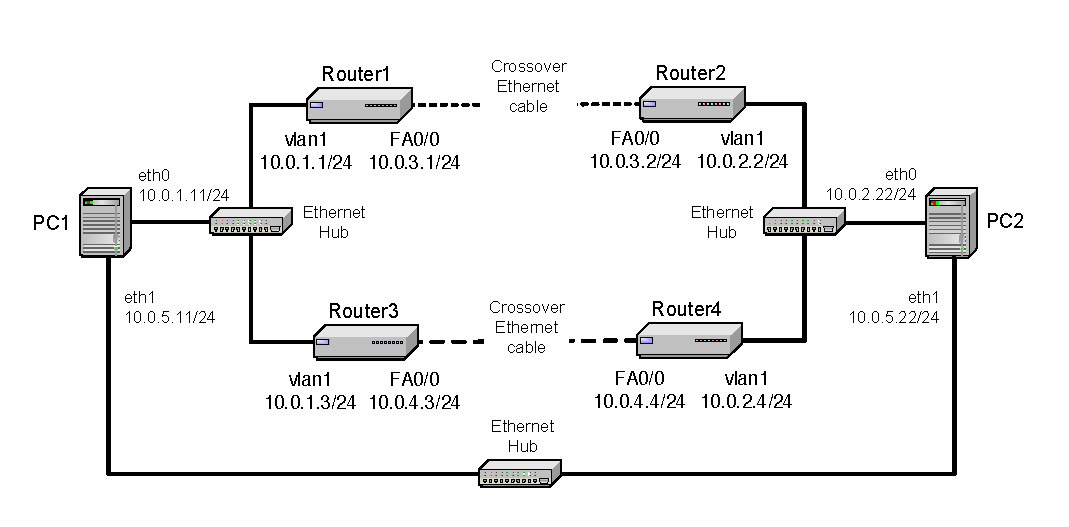
\includegraphics[width=\linewidth]{graphics/fig-5-2-updated.pdf}	
	\caption{Network Topology for Parts 1-4.}
	\label{fig:lab5-network-topology2}
\end{figure}


\begin{table}[ht]
	\centering
	\begin{tabular}{ |c c c| }
		\hline
		\textbf{Linux PC} & \textbf{Interface eth0} & \textbf{Interface eth1} \\ \hline
		PC1 & 10.0.1.11/24 & 10.0.5.11/24 \\ 
		PC2 & 10.0.2.22/24 & 10.0.5.22/24 \\ \hline
		\textbf{Cisco Router} & \textbf{Interface FastEthernet0/0} & \textbf{Interface vlan1} \\ \hline
		Router1 & 10.0.3.1/24 & 10.0.1.1/24 \\ 
		Router2 & 10.0.3.2/24 & 10.0.2.2/24 \\ \hline
		\textbf{Cisco Router} & \textbf{Interface FastEthernet0/0} & \textbf{Interface vlan1} \\ \hline
		Router3 & 10.0.4.3/24 & 10.0.1.3/24 \\ 
		Router4 & 10.0.4.4/24 & 10.0.2.4/24 \\ \hline
	\end{tabular}
	\caption{IP Addresses of Linux PCs and Cisco routers.}
	\label{tab:lab5-ip-addresses-2}
\end{table}

\begin{table}[ht]
	\centering
	\begin{tabular}{ |c | c c |}
		\hline
		\textbf{Linux PC} & \multicolumn{2}{c|}{\textbf{Routing Table Entries}} \\
		 & \textbf{Destination} & \textbf{Next Hop} \\ \hline
		PC1 & default gateway & 10.0.1.3 \\ \hline
		PC2 & default gateway & 10.0.2.4 \\ \hline
		\textbf{Linux PC} & \multicolumn{2}{c|}{\textbf{Routing Table Entries}} \\
		 & \textbf{Destination} & \textbf{Next Hop} \\ \hline
		Router1 & network 10.0.4.0/24 & 10.0.1.3 \\ 
		Router1 & default gateway & 10.0.3.2 \\ \hline
		Router2 & network 10.0.4.0/24 & 10.0.2.4 \\ 
		Router2 & default gateway & 10.0.3.1 \\ \hline
		Router3 & network 10.0.3.0/24 & 10.0.1.1 \\ 
		Router3 & default gateway & 10.0.4.4 \\ \hline
		Router4 & network 10.0.3.0/24 & 10.0.2.2 \\ 
		Router4 & default gateway & 10.0.4.3 \\ \hline
	\end{tabular}
	\caption{Routing table entries for Part 5-8.}
	\label{tab:lab5-routing-entries-part5-8}
\end{table}

\subsubsection{Exercise 5-a. Network Setup}

The following network configuration is used in the remaining parts of the lab.

\begin{enumerate}
	\item Set up the Ethernet connections as shown in Figure \ref{fig:lab5-network-topology2}. \emph{Note: connect two routers through a hub or switch if you don't have a crossover cable available.}
	\item Configure the IP addresses and the routing tables of the PCs as shown in Tables \ref{tab:lab5-ip-addresses-2} and \ref{tab:lab5-routing-entries-part5-8}.
		\begin{itemize}
			\item IP forwarding should be disabled on both PC1 and PC2.
			\item Set a new default gateways on PC1 and PC2. Remove the default gateway entry that was set in Part 1 of the lab. Changing the default gateway on PC1 is done with the following commands:
				\begin{cmdblock}
	PC1% route del default gw 10.0.1.33 
	PC1% route add default gw 10.0.1.3
				\end{cmdblock}
		\end{itemize}
		Repeat the steps on PC2. Use the command \cmd{netstat -rn}, to verify that there are no other static routing entries.
	\item Verify that the PCs are connected to the console ports of routers. PC1 should be connected to Router1, PC2 to Router 2, and so on. On each PC, establish a \cmd{minicom} session to the connected router.
	\item Configure the IP addresses and routing table entries of the routers. The commands for Router4 are as follows:
		\begin{cmdblock}
	Router4> enable
	Password: <enable secret>
	Router4# configure terminal
	Router4(config)# no ip routing
	Router4(config)# ip routing
	Router4(config)# ip route 0.0.0.0 0.0.0.0 10.0.4.3 
	Router4(config)# ip route 10.0.3.0 255.255.255.0 10.0.2.2 
	Router4(config)# interface FastEthernet0/0 
	Router4(config-if)# no shutdown
	Router4(config-if)# ip address 10.0.2.4 255.255.255.0 
	Router4(config-if)# interface FastEthernet0/1
	Router4(config-if)# no shutdown
	Router4(config-if)# interface vlan1
	Router4(config-if)# no shutdown
	Router4(config-if)# ip address 10.0.4.4 255.255.255.0
	Router4(config-if)# end
		\end{cmdblock}
		Use the commands \cmd{show ip route} and show interfaces to verify that the routing table and the interfaces are set correctly.
	\item Emulate a slow serial link between Router3 and Router4 using traffic-shaping:
		\begin{cmdblock}
	> interface FastEthernet0/0
	> ip address 10.10.1.80 255.255.255.0
	> fair-queue
	> traffic-shape rate 64000 5000 5000 1000
		\end{cmdblock}
		This will simulate a link of 64kbps on the packets going out of \iface{FE0/0}. You can change the parameters of the ``traffic-shape'' command to control the rate of the link. Don’t forget that shaping only works on the outgoing packets of the interface, so you will have to configure this in both Router3 and Router4! Also note that you can not apply the traffic shaping to a virtual interface like \iface{Vlan1}. You can use
		\begin{cmdblock}
	> show running-config
		\end{cmdblock}
		to check if the traffic shaping is correctly configured to 64kbps.
	\item Test the network connectivity by issuing ping commands between PC1 and PC2. Verify the route taken by traffic between the PCs by issuing \cmd{traceroute} commands.
		\begin{cmdblock}
	PC1% traceroute 10.0.2.22 PC1% traceroute 10.0.5.22
	PC2% traceroute 10.0.1.11 PC2% traceroute 10.0.5.11
		\end{cmdblock}
		Also, you should be able to issue ping commands between the routers. If the commands are not successful, use the commands \cmd{traceroute} (on Linux) or \cmd{trace} (on IOS) and the content of the routing tables to locate configuration problems.
\end{enumerate}
If all commands are successful, then you are ready to continue.

\subsubsection{Exercise 5-b. TCP Data Transfer - Interactive Applications over a fast link}

Here you observe interactive data transfer in TCP, by establishing a TCP connection from PC1 to PC2 over the Ethernet link between the PCs. Dependent on the type of hub, the Ethernet link has a maximum data rate of 10 Mbps or 100 Mbps.
\begin{enumerate}
	\item Start Wireshark on PC1 for interface \iface{eth1}, and start to capture traffic. Do not set any filters.
	\item On PC1, establish a Telnet session to PC2 by typing: 
		\begin{cmdblock}
	PC1% telnet 10.0.5.22
		\end{cmdblock}
		Log in as root user.
	\item Now start to type a few characters in the window which contains the Telnet session. The Telnet client sends each typed character in a separate TCP segment to the Telnet server, which, in turn, echoes the character back to the client. Including ACKs, one would expect to see four packets for each typed character. However, due to delayed acknowledgments, this is not the case.
		Observe the output of Wireshark:
\end{enumerate}

\textbf{Include your answers to the following questions. Include examples from the saved Wireshark data to support your answers.}
\begin{questions}
	\q{5.B.1.a}{Observe the number of packets exchanged between the Linux PCs for each keystroke? Describe the payload of the packets. Use your knowledge of delayed acknowledgements to explain the sequence of segment transmissions. Explain why you do not see four packets per typed character.}
	\q{5.B.1.b}{When the TCP client receives the echo of a character, it waits a certain time before sending the ACK. Why does the TCP client delay? How long is this delay? How much does the delay vary?}
	\q{5.B.1.c}{What is the time delay associated with the transmission of ACKs from the Telnet server on PC3?}
	\q{5.B.1.d}{Which flags, if any, are set in the TCP segments that carry typed characters as payload? Explain the meaning of these flags.}
	\q{5.B.1.e}{Why do segments that have an empty payload carry a sequence number? Why does this not result in confusion at the TCP receiver?}
	\q{5.B.1.f}{What is the window size that is advertised by the Telnet client and the Telnet server? How does the value of the window size field vary as the connection progresses?}
	\q{5.B.1.g}{Type characters in the Telnet client program as fast as you can, e.g., by pressing a key and holding it down. Do you observe a difference in the transmission of segment payloads and ACKs?}
\end{questions}

\begin{enumerate}[resume]
	\item Terminate the Telnet session by typing exit.
	\item Stop the traffic capture with Wireshark and save the captured packets.
\end{enumerate}

\begin{questions}
	\q{5.B.2}{For one character typed at the Telnet client, include a drawing that shows the transmission of TCP segments between PC1 and PC2 due to this character.}
\end{questions}
	
\subsubsection{Exercise 5-c. TCP Data Transfer - Interactive Applications over a slow link}

This exercise repeats the previous exercise, but establishes a data connection over the emulated slow link. The rate of this link should be set to 9600bps. This low rate introduces significant delays between PC1 and PC2. Due to the long delay, one would expect that the TCP sender transmits multiple segments, each carrying a payload of one typed character. However, this is not the case. A heuristic in TCP, called Nagle’s algorithm, forces the sender to wait for an ACK after transmitting a small segment, even if the window size would allow the transmission of multiple segments. Therefore, no matter how slow or fast you type, you should only observe one TCP segment in transmission at a time, when the TCP segments are small.

\begin{enumerate}
	\item Start to capture traffic with Wireshark on interface \iface{eth0} of PC1. Do not set any display filters.
	\item On PC1, establish a Telnet session to PC2 by typing: 
		\begin{cmdblock}
	PC1% telnet 10.0.2.22
		\end{cmdblock}
		Log in as root user. Note With the above IP address the route between PC1 to PC2 passes through the emulated serial link between Router3 and Router4.
	\item As, in the previous exercise, type a few characters in the window that contains the Telnet session. Vary the rate at which you type characters in the Telnet client program. Observe the output of Wireshark:
\end{enumerate}

\textbf{Include your answers to the following questions. For each answer, include Wireshark data to support your answer.}
\begin{questions}
	\q{5.C.1.a}{Observe the number of packets that are exchanged between the Linux PCs for each keystroke? Observe how the transmission of packets changes when you type characters more quickly.}
	\q{5.C.1.b}{Do you observe delayed acknowledgements? Why is the outcome expected?}
	\q{5.C.1.c}{If you type very quickly, i.e., if you hold a key down, you should observe that multiple characters are transmitted in the payload of a segment. Explain this outcome.}
\end{questions}

\begin{enumerate}[resume]
	\item Terminate the Telnet session by typing exit.
	\item Stop the traffic capture with Wireshark and save the captured packets.
\end{enumerate}

\begin{questions}
	\q{5.C.2}{Include an example from the saved Wireshark data, which shows that Nagle’s algorithm is used by the TCP sender.}
\end{questions}

\newpage
\subsection{TCP data exchange - Bulk data transfer}

The TCP receiver can use acknowledgements to control the transmission rate at the TCP sender. This is called flow control. Flow control is not an issue for interactive applications, since the traffic volume of these applications is small, but plays an important role in bulk transfer applications.

Bulk data transfers generally transmit full segments. In TCP, the receiver controls the amount of data that the sender can transmit using a sliding window flow control scheme. This prevents that the receiver gets overwhelmed with data. The number of bytes that the receiver is willing to accept is written in the window size field. An ACK that has values (250, 100) for the acknowledgement number and the window size is interpreted by the TCP sender, that the sender is allowed to transmit data with sequence numbers 250, 251,..., 359. The TCP sender may have already transmitted some data in that range.

In this part of the lab, you observe acknowledgements and flow control for bulk data transfers, where traffic is generated with the nttcp tool. To observe the bulk data transfer, we introduce a feature of Wireshark that allows you to view the data of a TCP connection in a graph. This is done in Exercise 6-c. We also show how to save the graphs to a file.

All exercises are done with the network configuration from Figure \ref{fig:lab5-network-topology2}.

\subsubsection{Exercise 6-a. TCP Data Transfer - Bulk transfer (Fast Link)}

The purpose of this exercise is to observe the operation of the sliding window flow control scheme in a bulk data transfer, where PC1 sends a large number of segments to PC2, using the nttcp traffic generation tool.
\begin{enumerate}
	\item The network configuration is the same as in Part 5. If the network is not set up accordingly, then follow the instructions in Exercise 5-a.
	\item Start Wireshark on PC1 for interface \iface{eth1}, and start to capture traffic. Do not set any display filters.
	\item Use nttcp to generate TCP traffic between PC1 and PC2.
		\begin{itemize}
			\item On PC2, start a nttcp receiving process by typing:
				\begin{cmdblock}
	PC2% nttcp -i -rs -l1000 -n500 -p4444
				\end{cmdblock}
			\item On PC1, start a nttcp sender process that sends 500 blocks of application data by typing:
				\begin{cmdblock}
	PC1% nttcp -ts -l1000 -n500 -p4444 -D 10.0.5.22
				\end{cmdblock}
		\end{itemize}
		By using 10.0.5.22 as destination address, traffic will go over through the direct Ethernet link between PC1 and PC2.
	\item From the output of Wireshark on PC1, observe the sliding window flow control scheme. The sender transmits data up to the window size advertised by the receiver and then waits for ACKs.
\end{enumerate}

\boxinfo{The outcome of this experiment is dependent on the data rate of the Ethernet link between PC1 and PC2. If PC1 and PC2 are connected directly by an Ethernet . crossover cable or by a dual-speed hub, they will most likely exchange traffic at a data rate of 100 Mbps. If the Linux PCs are connected by a 10 Mbps Ethernet hub, the data rate is limited accordingly. The rate of the connection has a big impact on the outcome of the experiment.}

\textbf{Include your answers to the following questions. Include captured traffic to support your answers.}
\begin{questions}
	\q{6.A.a}{Observe the transmission of TCP segments and ACKs. How frequently does the receiver send ACKs? Is there an ACK sent for each TCP segment, or less often. Can you determine the rule used by TCP to send ACKs? Can you explain this rule?}
	\q{6.A.b}{How much data (measured in bytes) does the receiver acknowledge in a typical ACK? What is the most data that is acknowledged in a single ACK?}
	\q{6.A.c}{What is the range of the window sizes advertised by the receiver? How does the window size vary during the lifetime of the TCP connection?}
	\q{6.A.d}{Select an arbitrary ACK packet in Wireshark sent by PC2 to PC1. Locate the acknowledgement number in the TCP header. Now relate this ACK to a segment sent by PC1. Identify this segment in the Wireshark output. How long did it take from the transmission of the segment, until the ACK arrives at PC1?}
	\q{6.A.e}{Determine whether, or not, the TCP sender generally transmits the maximum amount of data allowed by the advertised window. Explain your answer.}
	\q{6.A.f}{When the nttcp sender has transmitted all its data, it closes the connection, but acknowledgements from PC2 still trickle in. What does PC2 do when it has sent all ACKs?}
\end{questions}

\begin{enumerate}[resume]
	\item Stop the traffic capture with Wireshark and save the Wireshark output.
\end{enumerate}

\subsubsection{Exercise 6-b. TCP Data Transfer - Bulk transfer (Slow Link)}
This exercise repeats the previous experiment, with the exception that traffic is sent over the emulated serial link.

\begin{enumerate}
	\item Set the data rate of the serial link to 125 kbps. As in Exercixe-5b, this is done by using the traffic-shaping option.
	\item Create a new Wireshark session on PC1 for interface \iface{eth0}, and start to capture traffic. Do not set any display filters.
	\item Use nttcp to generate TCP traffic between PC1 and PC2.
		\begin{itemize}
			\item On PC2, start a nttcp receiving process by typing:
				\begin{cmdblock}
	PC2% nttcp -i -rs -l1000 -n500 -p4444
				\end{cmdblock}
			\item On PC1, start a nttcp sender process that sends 500 blocks of application data by typing:
				\begin{cmdblock}
	PC1% nttcp -ts -l1000 -n500 -p4444 -D 10.0.2.22
				\end{cmdblock}
		\end{itemize}
		With the given destination address, traffic will go through the slow serial link.
	\item Observe the differences to the data transmission in the previous exercise.
	\item Stop the traffic capture with wireshark and save the wireshark output.
\end{enumerate}

\textbf{Include your answers to the following questions. Emphasize the differences to the observations made in Exercise 6-a.}
\begin{questions}
	\q{6.B.a}{How does the pattern of data segments and ACK change, as compared to the fast Ethernet link?}
	\q{6.B.b}{Does the frequency of ACKs change?}
	\q{6.B.c}{Is the range of window sizes advertised by the receiver different from those in 6-a?}
	\q{6.B.d}{Does the TCP sender generally transmit the maximum amount of data allowed by the advertised window? Explain your answer.}
\end{questions}

\subsubsection{Exercise 6-c. View a graph of TCP data transfer}
Wireshark can generate graphs that illustrate the transmissions of segments on a PC connection. This exercise familiarizes you with the graphing capabilities of Wireshark, and shows how you can extract information from the graphs.

\begin{enumerate}
	\item \textbf{Select a TCP connection:} In the Wireshark main window, select a packet from the TCP connection for which you want to build a graph.
		\begin{itemize}
			\item Here, select a TCP packet sent from PC1 to PC2 in Exercise 6-b.
		\end{itemize}
	\item \textbf{Select the type of graph:} Select the Statistics menu from the Wireshark main window, and then select TCP Stream Analysis in the pull down menu, as shown in Figure 5.3. This displays the plotting functions available in Wireshark:
		\begin{figure}[ht]
			\centering
			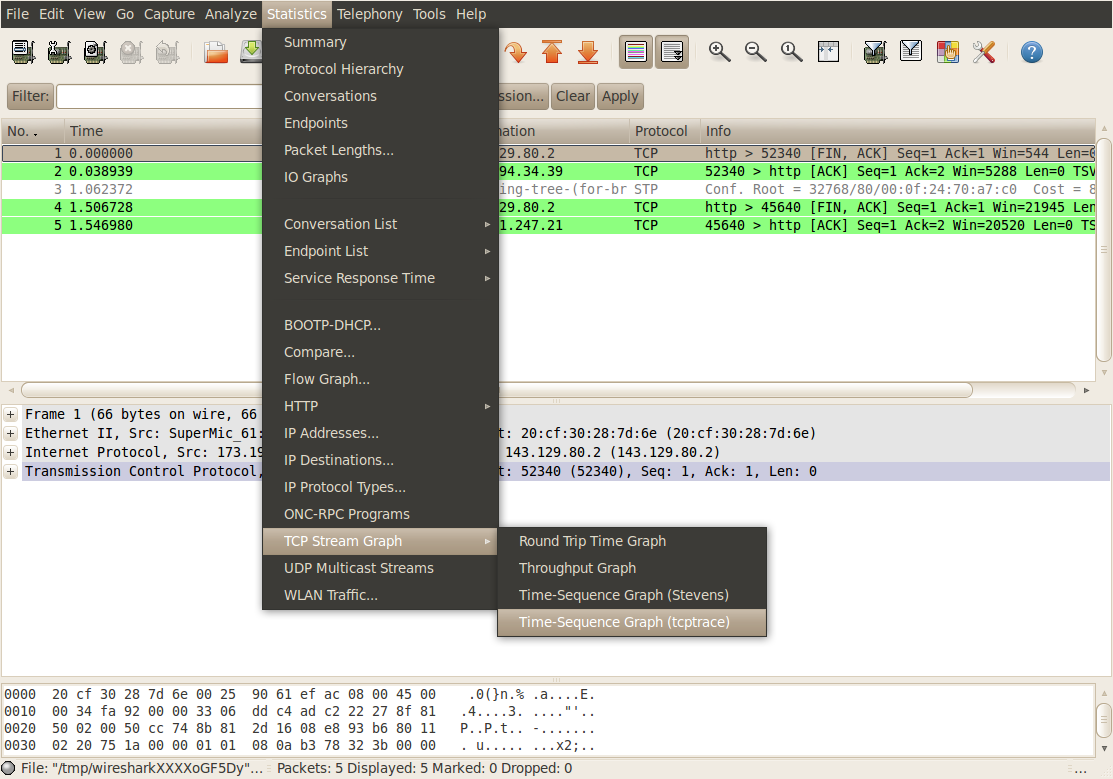
\includegraphics[width=\linewidth]{graphics/fig-5-3-updated.png}	
			\caption{Selecting the type of graph for a TCP connection.}
			\label{fig:lab5-type-of-tcp-graph}
		\end{figure}
		\begin{figure}[ht]
			\centering
			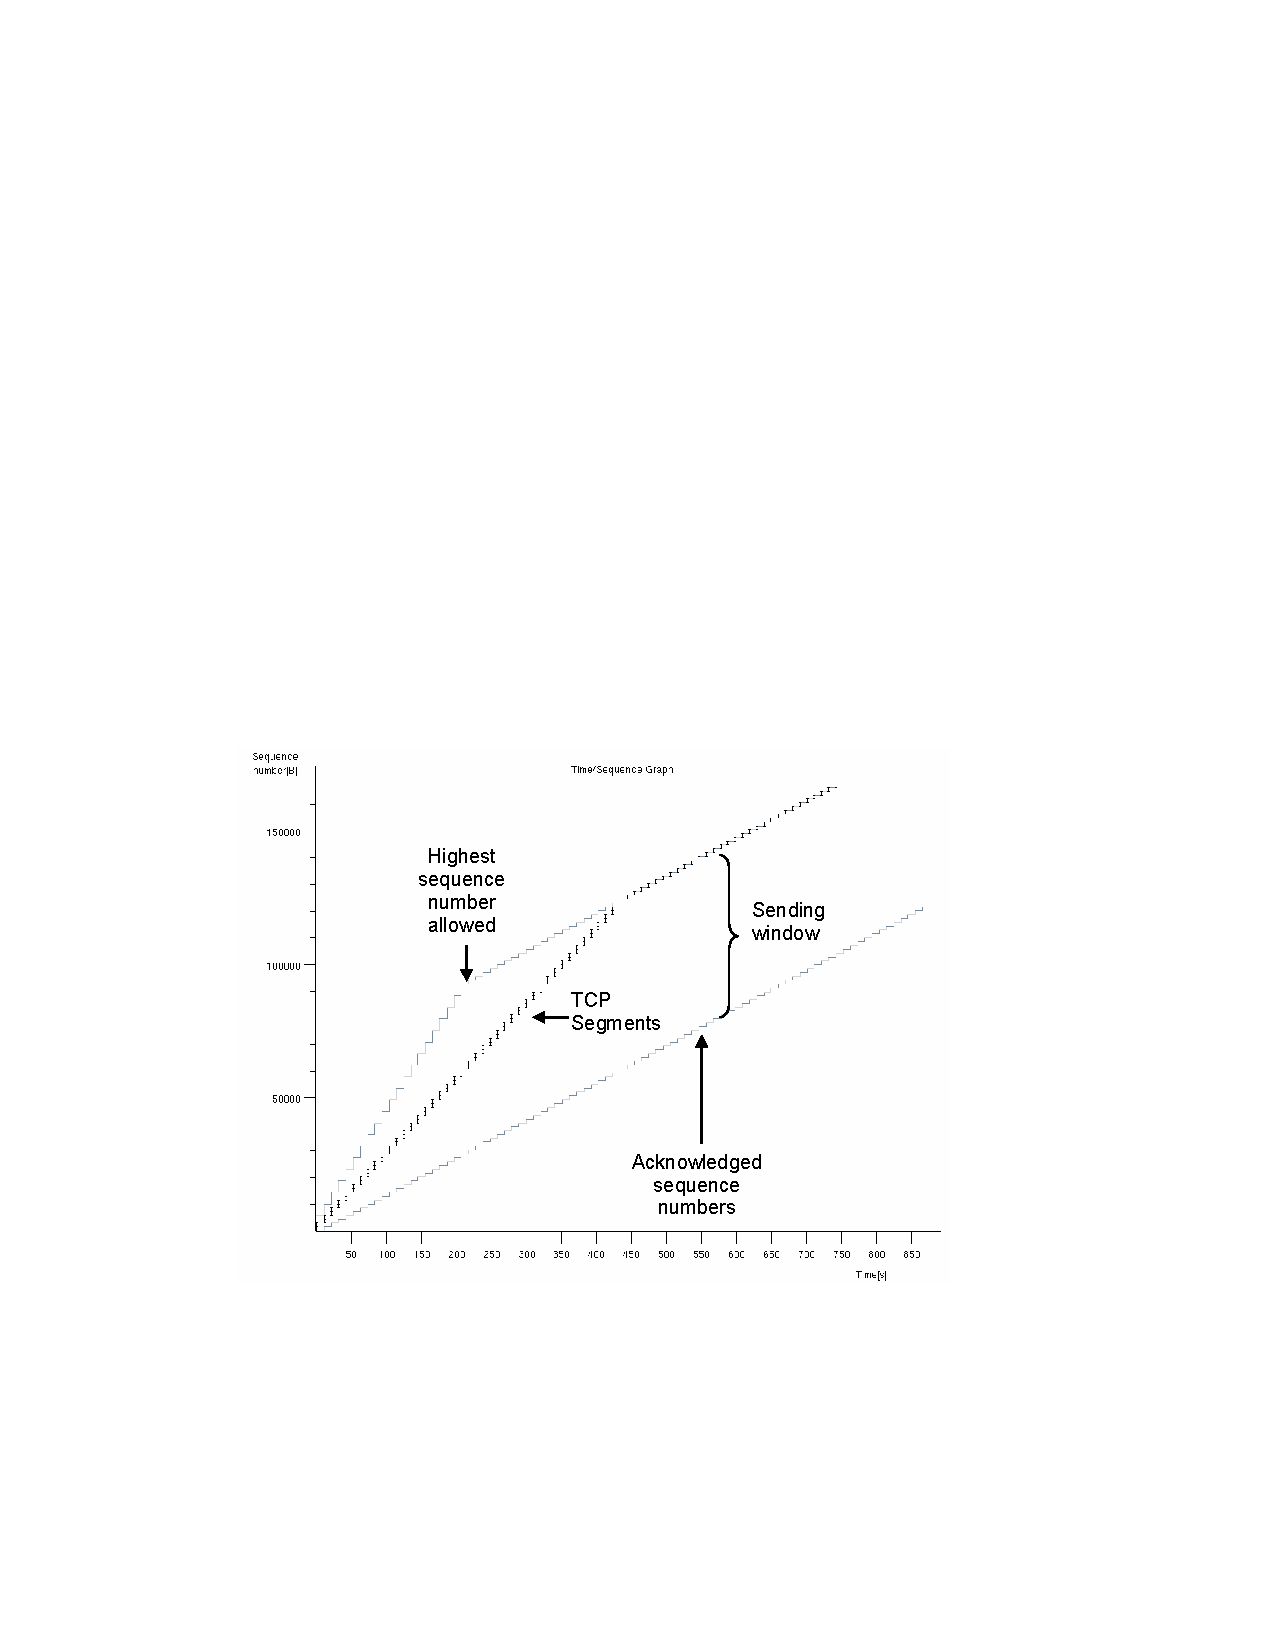
\includegraphics{graphics/fig-5-4-updated.pdf}	
			\caption{Time-Sequence Graph (tcptrace).}
			\label{fig:lab5-time-sequence}
		\end{figure}
		\begin{description}
			\item[Time-Sequence Graph (Stevens)] Plots the transmission of sequence numbers as a function of time. There is one data point for each transmission of a TCP segment.
			\item[Time-Sequence Graph (tcptrace)] Generates a plot as shown in Figure 5.4. The graph is similar to the previous one, but additional information is included on the state of the sliding window.
			\item[Throughput Graph] Shows the rate of data transmission as a function of time.
			\item[RTT Graph] Shows the roundtrip time (RTT) as a function of time.
		\end{description}
		Try out each of the graphs for the TCP connection from Exercise 6-b. Make sure that you select a packet with TCP payload from PC1 to PC2 in the Wireshark main window, before you generate a graph.
	\item \textbf{Navigating the graphs:} It is possible to navigate the graphs generated by Wireshark. For example, you can zoom into a graph to display an area of interest at a greater level of detail. Here is the complete set of available options:
		\begin{table}[ht]
			\centering
			\begin{tabular}{ | l p{8cm} | }
				\hline
				\textbf{Left mouse button} & Selecting a data point highlights the corresponding segment in the Wireshark main window. \\
				\textbf{Middle mouse button} & Zooms to a selected part of the graph. \\
				\textbf{Shift + Middle mouse button} & Zooms out. \\
				\textbf{Right mouse button} & Holding this button down and moving the mouse, moves the displayed section of the graph. This only works if the graph is zoomed in. \\
				\textbf{Ctrl + Right Button} & Magnifies a small portion of the graph. \\
				\textbf{Space} & Toggles between showing and not showing crosshairs. \\
				\textbf{s} & Toggles between relative and absolute sequence numbers. \\
				\textbf{t} & Toggles the display of the x-axis. \\ \hline
			\end{tabular}
			\caption{\textbf{Navigating graphs of TCP connection in Wireshark:}}
		\end{table}
	\item \textbf{Interpreting the Time-Sequence Graph (tcptrace):} A lot of information can be extracted from the Time-Sequence Graph (tcptrace). Refer to Figure 5.4 of a TCP connection. This graph shows the transmission of TCP segments and acknowledgements. The short vertical bars indicate the transmission of TCP segments. Each short bar represents one TCP segment, and the length of a bar corresponds to the length of a segment. The figure also shows two step curves. The top step curve shows the highest allowed sequence number, and the bottom step curve shows the acknowledged sequence numbers. These functions are determined from the acknowledgement number and the window size fields of received ACKs. The vertical distance between the two step curves shows the open part of the sliding window, that is, the sequence numbers that the TCP sender may transmit.\\
		From Figure 5.4, you can see that most of the time, TCP segments are transmitted in groups of two segments. An inspection of the vertical plot shows that no segments are retransmitted. The figure shows that the sequence numbers of transmitted segments are close to the upper step curve. This indicates that the TCP sender utilizes the entire sliding window, and that the transmissions by the TCP sender are triggered by arrivals of ACKs from the TCP receiver.
		\begin{itemize}
			\item Study the Time-Sequence Graph (tcptrace) of the TCP connections in Exercise 6-a and Exercise 6-b. Review the questions in Step 4 of Exercise 6-a and Step 3 in Exercise 6-b, and try to determine the answers to the questions directly from the graphs.
		\end{itemize}
	\item \textbf{Saving graphs to a file:} Unfortunately, Wireshark does not allow you to save the graphs for a TCP connection. However, there is a simple method in Linux to save a window on the desktop to a file.
Suppose you have constructed a TCP graph, similar to that of Figure 5.4, on PC1 and want to save it as a TIFF file. This is done by typing
		\begin{cmdblock}
	PC1% import lab6c.tif
		\end{cmdblock}
		and then clicking on the window with the TCP graph. This saves the graph to a TIFF file with name \path{lab6c.tif}. If you use a different file extension, the file is saved to a different image format. Select a file format that you can use in your lab report and that has sufficient image quality. The import command supports numerous file formats, including those in Table 5.5. We recommend that you use the TIFF file format, which offers the highest quality image. The size of the file can be reduced to less than 20 kB if you compress the file following the instructions below.
		\begin{table}[ht]
			\centering
			\begin{tabular}{ | c | c | c |}
				\hline
				\textbf{File extension} & \textbf{Format} & \textbf{approximate size of resulting file} \\ \hline
				.jpeg & JPEG & 30kB \\ \hline
				.eps & Encapsulated Postscript & 3.5 MB \\ \hline
				.gif & GIF & 300kB \\ \hline
				.tif & TIFF & 3.5MB \\ \hline
				\end{tabular}
			\caption{File formats for import command.}
			\label{tab:lab5-file-formats}
		\end{table}
		\begin{itemize}
			\item Save the Time-Sequence Graph (\cmd{tcptrace}) that you created for the TCP connections in Exercise 6-a and Exercise 6-b. Select a file format that you can use in your lab report. If you want to include detailed areas from the graphs, you may want to save multiple files for each graph.
			\item Verify the file has been correctly saved.
		\end{itemize}
\end{enumerate}

\begin{questions}
	\q{6.C}{Include the Time-Sequence Graph (\cmd{tcptrace}) graphs that you saved. You may also use these graphs for your answers to the lab report questions for Exercise 6-a and Exercise 6-b.}
\end{questions}
	
\newpage
\subsection{Retransmissions in TCP}
Next you observe retransmissions in TCP. TCP uses ACKs and timers to trigger retransmissions of lost segments. A TCP sender retransmits a segment when it assumes that the segment has been lost. This occurs in two situations:

\begin{enumerate}
	\item No ACK has been received for a segment. Each TCP sender maintains one retransmission timer for the connection. When the timer expires, the TCP sender retransmits the earliest segment that has not been acknowledged. The timer is started when a segment with payload is transmitted and the timer is not running, when an ACK arrives that acknowledges new data, and when a segment is retransmitted. The timer is stopped when all outstanding data has been acknowledged.\\
		The retransmission timer is set to a retransmission timeout (RTO) value, which adapts to the current network delays between the sender and the receiver. A TCP connection performs round-trip measurements by calculating the delay between the transmission of a segment and the receipt of the acknowledgement for that segment. The RTO value is calculated based on these round-trip measurements (see RFC 2988 from the prelab). Following a heuristic which is called Karn’s algorithm, measurements are not taken for retransmitted segments. Instead, when a retransmission occurs, the current RTO value is simply doubled.
	\item Multiple ACKs have been received for the same segment. A duplicate acknowledgement for a segment can be caused by an out-of-order delivery of a segment, or by a lost packet. A TCP sender takes multiple, in most cases three, duplicates as an indication that a packet has been lost. In this case, the TCP sender does not wait until the timer expires, but immediately retransmits the segment that is presumed lost. This mechanism is known as fast retransmit. The TCP receiver expedites a fast retransmit by sending an ACK for each packet that is received out-of-order.\\
		A disadvantage of cumulative acknowledgements in TCP is that a TCP receiver cannot request the retransmission of specific segments. For example, if the receiver has obtained segments 1, 2, 3, 5, 6, 7 cumulative acknowledgements only permit to send ACK for segments 1, 2, 3 but not for the other correctly received segments. This may result in an unnecessary retransmission of segments 5, 6, and 7. The problem can be remedied with an optional feature of TCP, which is known as selective acknowledgement (SACKs). Here, in addition to acknowledging the highest sequence number of contiguous data that has been received correctly, a receiver can acknowledge additional blocks of sequence numbers. The range of these blocks is included in TCP headers as an option. Whether SACKs are used or not, is negotiated in TCP header options when the TCP connection is created.
\end{enumerate}

The exercises in this part explore aspects of TCP retransmissions that do not require access to internal timers. Unfortunately, the roundtrip time measurements and the RTO values are difficult to observe, and are, therefore, not included in this lab.

The network configuration for this part is the network shown in Figure \ref{fig:lab5-network-topology2}.

\subsubsection{Exercise 7-a. TCP Retransmissions}

The purpose of this exercise is to observe when TCP retransmissions occur. As before, you transmit data from PC1 to PC2. Here, data is sent over the serial link, which is set to 125 kbps. When you disconnect one of the cables of the network, ACKs cannot reach the sending host. As a result, a timeout occurs and the sender performs retransmissions.

\begin{enumerate}
	\item The network configuration is the same as in Part 5. If the network is not setup accordingly, then follow the instructions in Exercise 5-a.
	\item Set the data rate of the emulated serial link to 125 kbps. If you continue from Part 6, this is the current value of the data rate of the link. If not, you proceed as in Exercise 5-a by setting the the traffic-shaping.
	\item Start Wireshark on PC1 and capture traffic on interface \iface{eth0}. Set a display filter to TCP traffic. This is done by typing \cmd{tcp} in the window at the bottom of the main window of Wireshark, next to the label Filter.
	\item Start a nttcp receiving process on PC2:
		\begin{cmdblock}
	PC2% nttcp -i -rs -l1000 -n500 -p4444
		\end{cmdblock}
	\item Start a nttcp sending process on PC1:
		\begin{cmdblock}
	PC1% nttcp -ts -l1000 -n500 -p4444 -D 10.0.2.22
		\end{cmdblock}
\end{enumerate}

\begin{questions}
	\q{7.A.5}{When the connection is created do the TCP sender and TCP receiver negotiate to permit SACKs? Describe the process of the negotiation.}
\end{questions}

\begin{enumerate}[resume]
	\item Once Wireshark has transmitted at least one hundred packets, disconnect the cable that connects \iface{FastEthernet0/0} of Router3 to the Ethernet hub. Disconnect the cable at the hub. Wait at least five minutes before you reconnect the cable. Observe TCP retransmissions from PC1 in the output of Wireshark.
\end{enumerate}

\begin{questions}
	\q{7.A.6.a}{Observe the time instants when retransmissions take place. How many packets retransmitted at one time?}
	\q{7.A.6.b}{Try to derive the algorithm that sets the time when a packet is retransmitted. (Repeat the experiment, if necessary). Is there a maximum time interval between retransmissions?}
	\q{7.A.6.c}{After how many retransmissions, if at all, does the TCP sender give up with retransmitting the segment? Describe your observations.}
\end{questions}

\begin{enumerate}[resume]
	\item Now reconnect the cable, and wait until the transmission resumes (This may take some time). Now quickly disconnect and reconnect the cable that connects the interface \iface{FastEthernet0/0} of Router3 to the Ethernet hub. Repeat this procedure a number of times, by varying the length of time that the cable is disconnected. Now observe the retransmissions from PC1.
\end{enumerate}

\begin{questions}
	\q{7.A.7}{Are the retransmissions different from those in Step 6? Specifically, do you observe fast retransmits and/or SACKs?}
\end{questions}

\begin{enumerate}[resume]
	\item Use the instructions from Exercise 6-c to build a Time-Sequence Graph (tcptrace) in Wireshark for the TCP connection. Study the output of the graph and use the graph to provide answers to the questions above. Use the navigating features to zoom in to parts of the graph that are of interest.
	\item Follow the instructions from Exercise 6-c to generate image files for the Time- Sequence Graph (tcptrace). Save enough images so that you can use the graphs to answer the above questions in your lab report. Generate images that show clearly the retransmission attempts in Step 6 and Step 7.
\end{enumerate}

\begin{questions}
	\q{7.A.9}{Include the image files saved in Step 9, and use them to support your answers. Annotate the graphs as necessary.}
\end{questions}


\subsubsection{Exercise 7-b. TCP performance at an overloaded link}

Next you perform an experiment, where you overload the emulated serial link between Router3 and Router4, and cause losses and retransmissions due to buffer overflows at Router3.

As in Exercise 7-a, you set up a TCP connection from PC1 to PC2. Here, however, you flood Router 3 with ICMP Echo Request messages. The purpose of this exercise is to observe how a TCP connection performs when a router is overloaded.
\begin{enumerate}
	\item Set the data rate of the serial link to 64 kbps. 
	\item Start Wireshark on PC1 for interface \iface{eth0} interface, and start to capture traffic. Set a display filter to TCP traffic.
	\item Start a nttcp receiving process on PC2:
		\begin{cmdblock}
	PC2% nttcp -i -rs -l1000 -n500 -p4444
		\end{cmdblock}
	\item Start a nttcp sending process on PC1:
		\begin{cmdblock}
	PC1% nttcp -ts -l1000 -n500 -p4444 -D 10.0.2.22
		\end{cmdblock}
	\item Once Wireshark has transmitted at least one hundred TCP packets, start to flood ICMP Echo Request messages by typing on PC1
		\begin{cmdblock}
	PC1% ping -f 10.0.2.22
		\end{cmdblock}
		Recall that with the \cmd{-f} option, PC2 sends ICMP Echo Request packets as fast as possible. The ICMP traffic sent from PC1 to PC2 will overflow the buffers of Router3 at the serial link.
	\item Follow the instructions from Exercise 6-c to build a Time-Sequence Graph (tcptrace) in Wireshark for the TCP connection. If you do not observe any retransmissions, reduce the data rate of the serial link. As long as the nttcp sender is transmitting packets, rerun the construction of the graph to observe how the graph changes as time progresses. In the graph, observe the progress of the TCP connection:
	\item Follow the instructions from Exercise 6-c to generate image files for the Time- Sequence Graph (tcptrace) and Throughput Graph. Save enough images so that you can use the graphs to answer the above questions in your lab report. Generate an image that shows in detail the loss events that occur right after the ping command is started.
\end{enumerate}

\begin{questions}
	\q{7.B}{Include your answers to the questions in Step 6. Included the saved image files from step 7. Annotate and describe the plots to support your answers.}
	\q{7.B.6.a}{Describe the losses that occur in the graph when the ping command is started. Do losses occur in regular intervals or irregularly?}
	\q{7.B.6.b}{From the graph, describe the size of the advertised window changes when the flooding ping is started.}
	\q{7.B.6.c}{Try to determine if retransmissions occur due to fast retransmit or due to timeouts of the timers. How can you determine which type of retransmissions you observe?}
	\q{7.B.6.d}{Generate a Throughput Graph to view the data rate of the TCP connection. How does the throughput change after the flood of pings is started?}
\end{questions}

\newpage
\subsection{TCP Congestion Control}

TCP congestion control consists of a set of algorithms that adapt the sending rate of a TCP sender to the current conditions in the network. When the network is not congested, the TCP sender is allowed to increase its sending rate, and when the network is congested, the TCP sender reduces its rate. The TCP sender maintains a congestion window which limits the number of segments that can be sent without waiting for an acknowledgement. The actual number of segments that can be sent is the minimum of the congestion window and the window size sent by the receiver.

For congestion control, each TCP sender keeps two variables, the congestion window (cwnd) and the slow-start threshold (ssthresh). The initial values are set to one segment for cwnd and 65535 bytes for ssthresh. TCP congestion control operates in two phases, called slow start and congestion avoidance. The sender is in the slow start phase when cwnd $\le$ ssthresh. Here, cwnd is increased by one for each arrived ACK. This results in a doubling of cwnd for each roundtrip time. When cwnd \textgreater  ssthresh, the TCP sender is in the congestion avoidance phase. Here, the cwnd is incremented by one only after cwnd ACKs. This is done by incrementing cwnd by a fraction of a segment when an ACK arrives.

The TCP sender assumes that the network is congested when a segment is lost, that is, when the retransmission timer has a timeout or when three duplicate ACKs arrive. When a timeout occurs, the TCP sender sets ssthresh to half the current value of cwnd and then sets cwnd to one. This puts the TCP sender in slow start mode. When a third duplicate ACK arrives, the TCP sender performs what is called a fast recovery. Here, ssthresh is set to half the current value of cwnd, and cwnd is set to the new value of ssthresh.

The goal of this part of the lab is to observe the development of the congestion window. Since the number of the segments that can be transmitted by a TCP sender is the result of the congestion window as well as the advertised window, and since data segments and returning ACKs interleave, the size of the congestion window is not derived by observing traffic.

\subsubsection*{Exercise 8-a. Network Setup}

The network configuration used is that in Figure \ref{fig:lab5-network-topology2}. To observe the slow start features, change the routing table entries so that traffic from PC1 to PC2 traverses the path PC1 $\rightarrow$ R1 $\rightarrow$ R2 $\rightarrow$ PC2, and the reverse path is PC2 $\rightarrow$ R4 $\rightarrow$ R3 $\rightarrow$ PC1. When PC1 sends data to PC2, data segments can be transmitted quickly to PC2, but ACKs only slowly return to PC1. The sender will therefore transmit a full window of packets up to the threshold of the congestion window, and then be forced to wait to receive the ACKs before transmitting the next batch of packets.

\begin{enumerate}
	\item The network configuration is similar to that in Parts 5-7. If the network is not setup accordingly, then follow the instructions in Exercise 5-a. The following two steps are modifications to the setup of Exercise 5-a.
	\item Set a new default gateway of PC1 to Router1. If the default gateway from Table 5.4 is still set, you must first delete the existing entry. Use the command \cmd{netstat -rn} to see if a default gateway is configured. Assuming that the configuration from Table 5.4, you must enter the following commands:
		\begin{cmdblock}
	PC1% route del default gw 10.0.1.3
	PC1% route add default gw 10.0.1.1
		\end{cmdblock}
		The default gateway of PC2 remains unchanged and should be as shown in Table \ref{tab:lab5-routing-entries-part5-8}.
		With this modification, traffic from PC1 to PC2 passes through Router1 and Router2, and traffic from PC2 to PC1 passes through Router4 and Router3. Verify that this is the case.
	\item Set the data rate of the emulated serial link to 1 Mbps.
\end{enumerate}

\subsubsection{Exercise 8-b. Observing TCP congestion control}

This exercise is similar to Exercise 6-a, that is, PC1 transmits TCP segments to PC2.
\begin{enumerate}
	\item Start Wireshark for interface \iface{eth0} on PC1, and start to capture traffic. Set a display filter to TCP traffic.
	\item Start a nttcp receiving process on PC2:
		\begin{cmdblock}
	PC2% nttcp -i -rs -l1000 -n5000 -p4444
		\end{cmdblock}
	\item Start a nttcp sending process on PC1 that transmits 5000 blocks of data, each with 1000 Bytes:
		\begin{cmdblock}
	PC1% nttcp -ts -l1000 -n5000 -p4444 -D 10.0.2.22
		\end{cmdblock}
	\item Once Wireshark has transmitted at least one hundred TCP packets, disconnect the cable that connects \iface{FastEthernet0/0} of Router1 to the Ethernet hub. Disconnect the cable at the hub. Now reconnect the cable, and wait until the transmission resumes. Repeat this for a few times, varying the durations when the cable is disconnected.
	\item Use the instructions from Exercise 6-c to build a Time-Sequence Graph (tcptrace) in Wireshark for the TCP connection. Study the graph at the time instants when the cable is reconnected and TCP sender resumes transmission. Use the navigating features to zoom in to parts of the graph that are of interest.
		\boxinfo{The outcome of this experiment is dependent on the data rate of the link between Router1 and Router2, and Router3 and Router4, respectively. The outcome of the experiment is different when the Ethernet link between Router1 and Router2 is running at 10 Mbps or at 100 Mbps. The above settings are optimized for a 10 Mbps Ethernet link between Router1 and Router2.}
	\item Follow the instructions from Exercise 6-c to generate image files for the Time- Sequence Graph (tcptrace). Save enough images so that you can use the graphs to answer the above questions in your lab report. Make sure you include an image that shows a portion of the graph that illustrates the slow start phase. Compress the files and copy the files to a floppy disk.
\end{enumerate}

\begin{questions}
	\q{8.B}{Include the answers to the questions from Step 5. Use the saved image files to support your answers. Annotate the events in this graph, and explain the events that you observe, e.g. segments dropped, retransmission, congestion window, slow start, congestion avoidance, fast recovery, etc.}
	\q{8.B.5.a}{Try to observe periods when the TCP sender is in a slow start phase and when the sender switches to congestion avoidance. Verify that the congestion window follows the rules of the slow start phase.}
	\q{8.B.5.b}{Can you deduct the size of the ssthresh parameter during the times when the congestion window is small?}
	\q{8.B.5.c}{Can you find occurrences of fast recovery?}
\end{questions}

\setcounter {chapter} {5}
%%!TEX root = labo.tex

\setcounter {chapter} {5} 

\chapter{LAN switching}

What you will learn in this lab:
\begin{itemize}
	\item How to configure a Cisco Router and a Linux PC as a LAN switch.
	\item How LAN switches update their forwarding tables.
	\item How LAN switches run a spanning tree protocol for loop free routing.
\end{itemize}

\newpage
\setsession{prelab6}
\section{Prelab 6}\label{sec:prelab6}
%!TEX root = labo.tex

\subsubsection*{Bridges and the Spanning Tree Protocol}
Use the following resources to prepare yourself for this lab session:
\begin{enumerate}
	\item Bridging: Read about LAN switching and bridging at \url{http://docwiki.cisco.com/wiki/Internetworking_Technology_Handbook#Bridging_and_Switching}.
	\item Transparent Bridges and Spanning Tree Protocol: Read about transparent bridges and the spanning tree protocol at \url{http://docwiki.cisco.com/wiki/Transparent_Bridging}.
	\item Bridge Protocol Data Unit (BPDU): Familiarize yourself with the format of bridge protocol data units (BPDUs) by reading the information at \url{http://ericleahy.com/index.php/implementing-spanning-tree-protocol-stp/}.
	\item Configuring a PC as a Bridge: Explore the website \url{http://www.linuxfoundation.org/collaborate/workgroups/networking/bridge}, which describes the bridge-utils software package for configuring a Linux PC as a bridge.
\end{enumerate}

\newpage
\subsection*{Prelab Questions}
\begin{questions}
	\q{1}{Describe the difference between a LAN switch/bridge and a router?}
	\q{2}{What is the difference between an Ethernet switch and an Ethernet hub? Which is more suitable for a network with a high traffic load, a switch or a hub? Explain.}
	\q{3}{What motivates the use of the term "transparent" in transparent bridges?}
	\q{4}{Which role does the spanning tree protocol play when interconnecting LAN switches/bridges?}
	\q{5.a}{In the context of the IEEE 802.1d specification of the spanning tree protocol, define root bridge.}
	\q{5.b}{In the context of the IEEE 802.1d specification of the spanning tree protocol, define root port.}
	\q{5.c}{In the context of the IEEE 802.1d specification of the spanning tree protocol, define designated bridge.}
	\q{5.d}{In the context of the IEEE 802.1d specification of the spanning tree protocol, define designated port.}
	\q{5.e}{In the context of the IEEE 802.1d specification of the spanning tree protocol, define blocked port.}
	\q{6}{In the spanning tree protocol, how does a LAN switch/bridge decide which ports are in a blocking state?}
\end{questions}


\newpage
\setsession{lab6}
\section{Lab 6}\label{sec:lab6}

A bridge or LAN switch is a device that interconnects two or more Local Area Networks (LANs) and forwards packets between these networks. Different from IP routers, bridges and LAN switches operate at the data link layer. For example, bridges and LAN switches forward packets based on MAC addresses, whereas IP routers forward packets based on IP addresses.

LAN switches are widely deployed in enterprise networks, including university campus networks. Many enterprise networks primarily use LAN switches, and use IP routers only to connect the enterprise network to the public Internet.

The term 'bridge' was coined in the early 1980s. Today, when referring to data-link layer interconnection devices, the terms 'LAN switch' or 'Ethernet switch' (in the context of Ethernet) are much more common. Since many of the concepts, configuration commands, and protocols for LAN switches in Lab 6 use the old term 'bridge', we will, with few exceptions, refer to LAN switches as bridges.

This lab covers the main concepts of LAN switching in Ethernet networks: how packets are forwarded between LANs and how the routes of packets are determined. In the first and second parts of Lab 6, you learn how to configure a Linux PC and a Cisco router as a bridge. The third part illustrates the difference between an Ethernet hub and an Ethernet switch. Parts 4 explores how forwarding tables of bridges are set up. You learn about the concepts of learning bridges and transparent bridges.

The configuration of the equipment in Lab 6 is changed several times during the course of the lab. With exception of the last part, the IP address configuration of the Linux PCs is as shown in Table \ref{tab:lab6-network1}. Note that all IP addresses have the same netmask.

\begin{table}[h!t]
\centering
	\begin{tabular}{| c | c | c |}	
		\hline
		\textbf{Linux PC} & \textbf{eth0} & \textbf{eth1} \\ \hline
		PC1 & 10.0.1.11/24 & 10.0.1.12/24 \\ 
		PC2 & 10.0.2.21/24 & 10.0.1.22/24 \\
		PC3 & 10.0.3.31/24 & 10.0.1.32/24 \\
		PC4 & 10.0.4.41/24 & 10.0.1.42/24 \\ \hline
	\end{tabular}
	\caption{IP addresses}
	\label{tab:lab6-network1}
\end{table}

\newpage
\subsection{Configuring a Linux PC as a bridge}

The exercises in this lab show how to configure a Linux PC as a bridge. Ethernet bridging functionality is integrated in all recent versions of Linux. The configuration of bridging functions in Linux is done with configuration commands and tools. In this lab, we use the command-line bridge configuration tool \cmd{brctl}.

The network configuration for this part is shown in Figure \ref{fig:lab6-network1}. Here, PC1 and PC3 act as hosts and PC2 is set up as a bridge.

\begin{figure}[h!t]
	\centering
	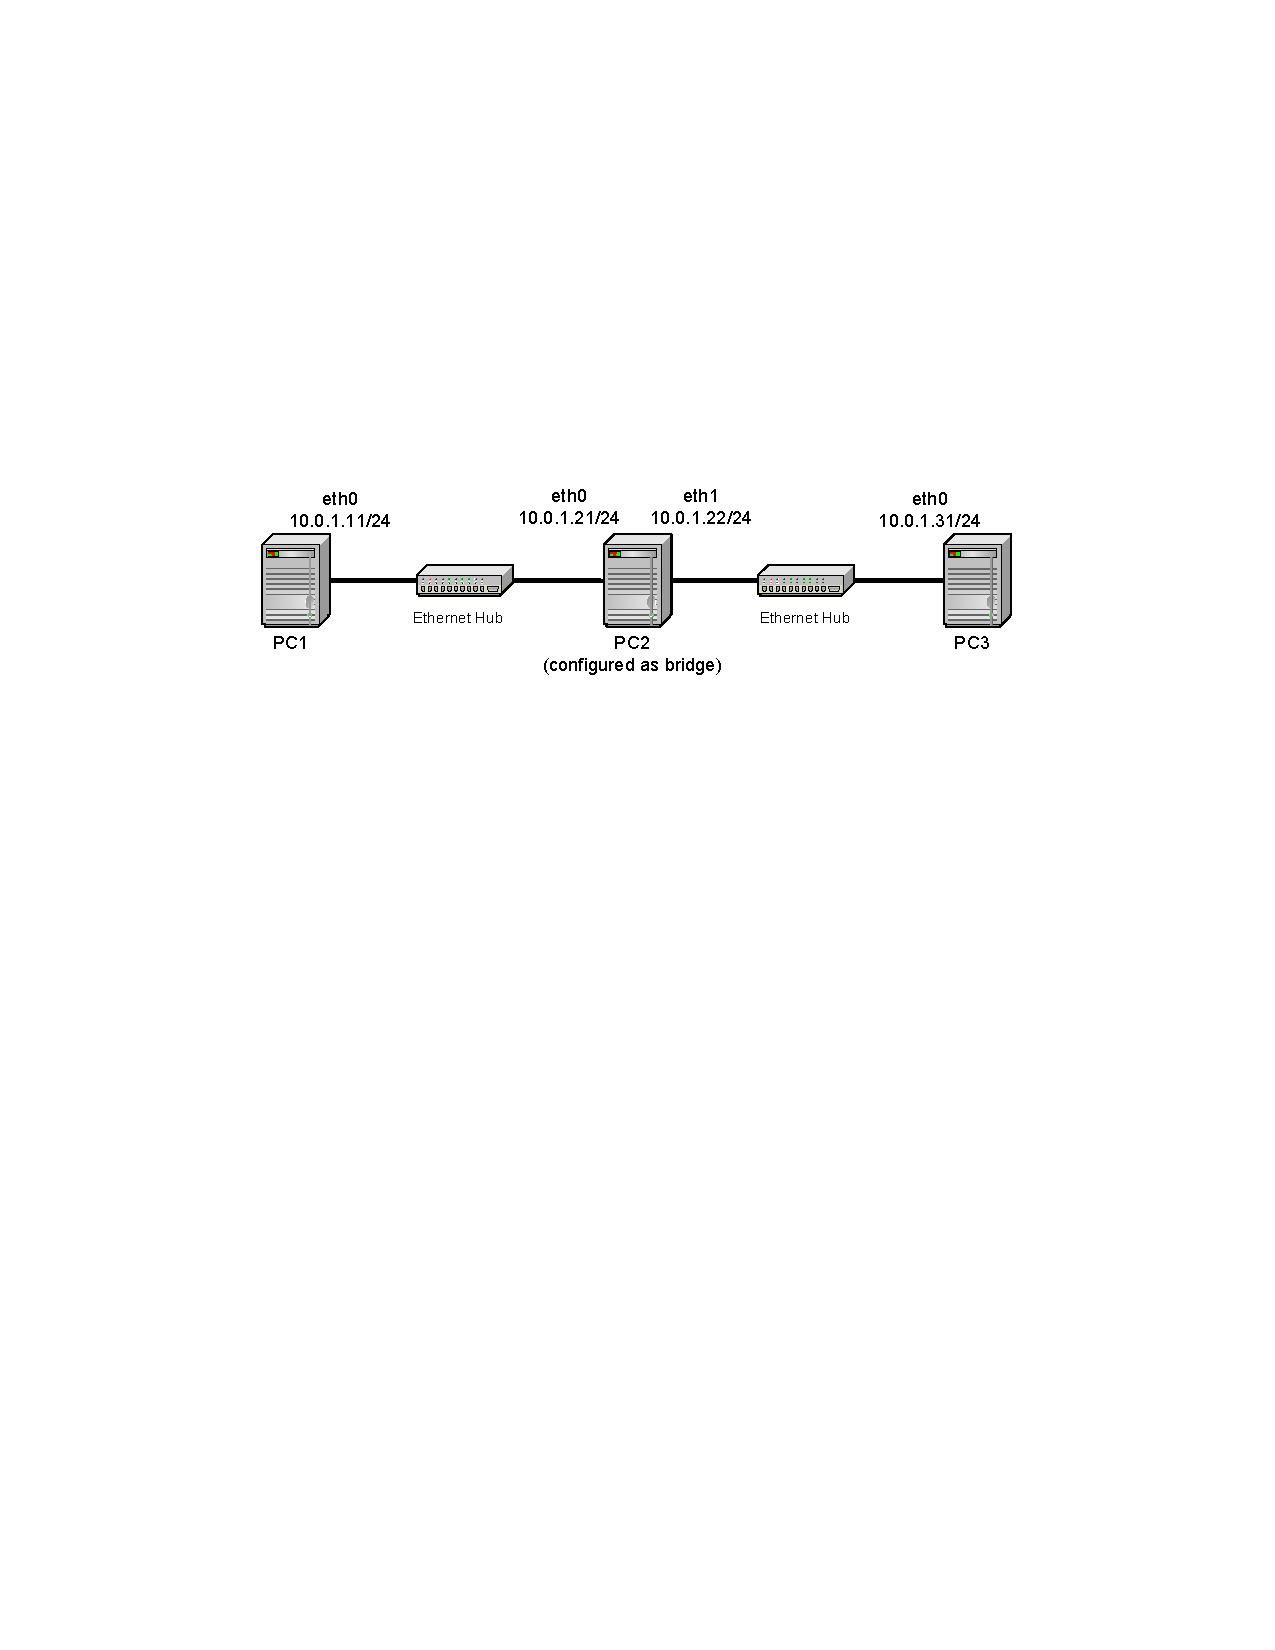
\includegraphics[width=\linewidth]{graphics/lab6-network1.pdf}	
	\caption{Network Topology for Part 1.}
	\label{fig:lab6-network1}
\end{figure}

\subsubsection{Exercise 1-a. IP configuration of Linux PCs}
\begin{enumerate}
	\item Set up the network configuration as shown in Figure \ref{fig:lab6-network1}.
	\item Configure the interfaces of PC1, PC2, and PC3, with the IP addresses given in Table \ref{tab:lab6-network1}. Disable the interfaces that are not used in the configuration, that is, disable interface \iface{eth1} on both PC1 and PC3.
	\item Since, throughout Lab 6, you frequently work with MAC addresses, you should record the MAC addresses of the Linux PCs. Log in to each of the PCs and obtain the MAC addresses of both Ethernet interfaces with the command \cmd{ifconfig -a}. Enter the MAC addresses in Table \ref{tab:lab6-macs-pcs}. (In Part 2, you will repeat the same exercise on the Cisco routers.)
		\begin{table}[h!t]
			\centering
			\begin{tabular}{| c | c | c |}	
				\hline
				\textbf{Linux PC} & \textbf{MAC address of eth0} & \textbf{MAC address of eth1} \\ \hline
				PC1 & 68:05:ca:36:33:a0 & 68:05:ca:39:cc:79 \\ 
				PC2 & 68:05:ca:36:31:f0 & 68:05:ca:39:e1:36 \\
				PC3 & 68:05:ca:36:39:c7 & 68:05:ca:36:51:3f \\
				PC4 & 68:05:ca:39:e1:2f & 68:05:ca:39:e1:32 \\ \hline
			\end{tabular}
			\caption{MAC addresses of the linux PCs}
			\label{tab:lab6-macs-pcs}
		\end{table}
\end{enumerate}

\subsubsection{Exercise 1-b. Configure a Linux PC as a bridge}
In this exercise, you configure PC2 as a bridge that forwards packets between the two Ethernet segments shown in Figure \ref{fig:lab6-network1}. The bridge configuration on the Linux PCs is done with the tool \cmd{brctl}.
\begin{enumerate}
	\item Creating a bridge with \cmd{brctl}: It is possible to configure multiple independently operating bridges on the same PC. Each bridge is assigned a name and is associated with a set of interfaces. Here, you configure one bridge on PC2 and assign the bridge the name Bridge1.
		\begin{cmdblock}
	brctl addbr Bridge1	
		\end{cmdblock}
		Check if the bridge has been created by typing:
		\begin{cmdblock}
	brctl show
		\end{cmdblock}
	\item Configuring a bridge with \cmd{brctl}: After the bridge is created, the bridge is configured in the following steps:
		\begin{itemize}
			\item Assign interfaces to the bridge. e.g. for PC2, add the interfaces \iface{eth0} and \iface{eth1}.
				\begin{cmdblock}
	brctl addif Bridge1 eth0
	brctl addif Bridge1 eth1
				\end{cmdblock}
			\item The next part of the configuration sets the parameters of the spanning tree protocol (STP). In Part 1, the spanning tree protocol is not used. Therefore, you need to disable the spanning tree protocol by toggling the button next to the STP label, so that it shows the label Disabled.
				\begin{cmdblock}
	brctl stp Bridge1 off
				\end{cmdblock}
			\item In the last part of the bridge configuration, you activate the bridge \iface{Bridge1} from a terminal window. On a Linux PC, each created bridge is represented as a network interface. Therefore, if you type the command ifconfig -a on PC2, the command shows an interface Bridge1, in addition to the other interfaces \iface{eth0}, \iface{eth1}, and \iface{lo}. The bridge is activated by enabling the interface associated with the bridge. This is done with the following command:
				\begin{cmdblock}
	PC1% ifconfig Bridge1 up
			\end{cmdblock}
			\boxwarning{Activating the bridge disables the IP configuration of the interfaces assigned to a bridge. Hence, it is no longer possible to issue ping commands to these interfaces.}
		\end{itemize}
\end{enumerate}

\boxinfo{The following settings can also be configured on a bridge interface. You don't need to change them for this exercise however.
	\begin{description}
		\item[\texttt{setageing <bridge> <time>}] \hfill \\
			Set ageing time to <time> for bridge interface \iface{<bridge>}
		\item[\texttt{setbridgeprio <bridge> <prio>}] \hfill \\
			Set bridge priority to <prio> for bridge interface \iface{<bridge>}
		\item[\texttt{setfd <bridge> <time>}] \hfill \\
			Set bridge forward delay to <time> for bridge interface \iface{<bridge>}
		\item[\texttt{sethello <bridge> <time>}] \hfill \\
			Set hello time to <time> for bridge interface \iface{<bridge>}
		\item[\texttt{setmaxage <bridge> <time>}] \hfill \\
			Set the maximum message age to <time> for bridge interface \iface{<bridge>}
		\item[\texttt{stp <bridge> {on|off}}] \hfill \\
			Turn the Spanning Tree Protocol on/off for bridge interface \iface{bridge}
	\end{description}
}


\subsubsection{Exercise 1-c. Observing a bridge in operation}
\boxwarning{You will use Wireshark in this exercise. Do not forget to append the binary dump (pcap format) to your lab report}

When the bridge configuration of PC2 is complete, PC2 forwards packets between PC1 and PC3. This exercise asks you to observe the forwarding.
\begin{enumerate}
	\item Start Wireshark on PC1 and PC3, and capture traffic on interface \iface{eth0} on both systems.
	\item When bridging is activated on PC2, the configured IP addresses on PC2 should be disabled. To verify this, issue a ping command to interfaces \iface{eth0} and \iface{eth1} of PC2 from PC1 and PC3.
		\begin{cmdblock}
	PC1% ping 10.0.1.21
	PC3% ping 10.0.1.22
		\end{cmdblock}
		If PC2 is configured as a bridge, these ping commands should fail.
	\item Clear the ARP caches on PC1 and PC3. Note that in Linux, each ARP entry has to be deleted separately with the command \cmd{arp -d <MACaddress>}.
	\item Issue a ping command from PC1 to PC3 and save the output.
		\begin{cmdblock}
	PC1% ping -c 1 10.0.1.31
		\end{cmdblock}
		Observe that PC2 actually forwards the packets between PC1 and PC3.
\end{enumerate}

\begin{questions}
\q{1.C.1}{Do the source and destination MAC/IP addresses change when a packet traverses a bridge? Provide an explanation and include an example from the captured data. Suppose that PC2 was configured as an IP router, which differences would you observe in the Ethernet and IP headers?}
\end{questions}

\begin{enumerate}[resume]
	\item Run \cmd{traceroute} from PC1 to PC3 and save the output 
		\begin{cmdblock}
	PC1% traceroute 10.0.1.31
		\end{cmdblock}
		Here, you should observe that PC2 does not appear in the output of \cmd{traceroute}.
\end{enumerate}

\begin{questions}
	\q{1.C.2}{Include the output from the \cmd{traceroute} command. Why is PC2 not visible from PC1?}
	\q{1.C.3}{If PC2 was configured as an IP router, how would the output differ?}
\end{questions}

\begin{enumerate}[resume]
	\item Change the IP address of PC3 to 10.0.2.12/24. Note that PC1 and PC3 now have different IP network prefixes. Repeat Step 4.
\end{enumerate}

\begin{questions}
\q{1.C.4}{Does the ping command from PC1 to PC3 still work? Explain the outcome.}
\end{questions}

\subsubsection{Exercise 1-d. Manipulating a PC bridge}

This exercise familiarizes you with a few tasks related to running \cmd{brctl} on a Linux PC. You learn how to display the MAC forwarding table, how to delete the contents of the MAC forwarding table, and, finally, how to turn off the bridging functions. All of the tasks are performed on PC2.
\begin{enumerate}
	\item First, reset the IP address of the \iface{eth0} interface of PC3 to 10.0.1.31/24.
	\item Displaying the MAC forwarding table: The MAC forwarding table of a bridge plays the same role as the routing table of an IP router. To view the contents of the MAC forwarding table of Bridge1 on PC2, perform the following steps:
		\begin{cmdblock}
	brctl showmacs Bridge1
		\end{cmdblock}
	\item Clearing the MAC forwarding table of a bridge: The \cmd{brctl} tool does not have a convenient way to delete the contents of the MAC forwarding table. Instead you must exploit that a bridge automatically deletes an entry in the forwarding table that has not been looked up for a certain time, which is determined by the ageing parameter of \cmd{brctl}. To delete the entries in the forwarding table, you must set the ageing parameter to zero seconds. Once the entries are deleted, set the Ageing entry back to the original value (The default value is 300 seconds).
		\begin{cmdblock}
	brctl setageing Bridge1 0
	brctl setageing Bridge1 300
		\end{cmdblock}
	\item Disabling a bridge: Disabling a bridge on a Linux PC is done in two steps: (1) deactivate the interface associated with \iface{Bridge1} and (2) delete the bridge.
		\begin{cmdblock}
	ifconfig Bridge1 down
	brctl delbr Bridge1
		\end{cmdblock}
		You can verify that the bridge is disabled as follows: Verify that PC2 is operating as a normal host. To do this, issue a ping command to interfaces \iface{eth0} and \iface{eth1} of PC2 from PC1 and PC3. 
		\begin{cmdblock}
	PC1% ping -c 1 10.0.1.21
	PC3% ping -c 1 10.0.1.22
		\end{cmdblock}
		Verify that PC2 does not forward packets by issuing the following ping command:
		\begin{cmdblock}
	PC1% ping -c 1 10.0.1.31
		\end{cmdblock}
		The ping command should not be successful.
\end{enumerate}


\newpage
\subsection{Configuring a Cisco Router as a bridge}

Next you learn how to configure a Cisco Router as a bridge. The topology for this part is shown in Figure \ref{fig:lab6-network2}. Router1 is configured as a bridge that connects the two Ethernet segments.

\begin{figure}[h!t]
	\centering
	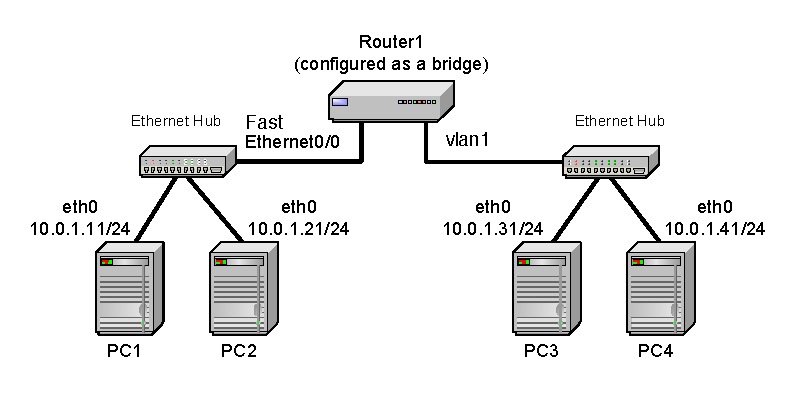
\includegraphics[width=\linewidth]{graphics/lab6-network2-updated.pdf}	
	\caption{Network Topology for Parts 2 and 3-b.}
	\label{fig:lab6-network2}
\end{figure}

\subsubsection{Exercise 2-a. Setup of network configuration}
After the network is configured, as in Exercise 1-a above for the Linux PCs, you are asked to record the MAC addresses of the Cisco routers.
\begin{enumerate}
	\item Connect the PCs and Router1 with Ethernet hubs as shown in Figure \ref{fig:lab6-network2}.
	\item Configure the \iface{eth0} interfaces of the Linux PCs with the IP addresses given in Table \ref{tab:lab6-network1}. (The IP addresses of PC1, PC2, and PC3 are the same as in Part 1). Disable the \iface{eth1} interfaces of all Linux PCs.
	\item Establish a \cmd{minimcom} session to each Cisco router: from PC1 to Router1, from PC2 to Router2, and so on.
	\item On each router, type \cmd{enable} and then use the command \cmd{show interfaces} to display the MAC addresses of the Ethernet interfaces. Record the MAC addresses in Table \ref{tab:lab6-macs-routers}.
		\begin{table}[h!t]
			\centering
			\begin{tabular}{| c | c | c |}	
				\hline
				\textbf{Linux PC} & \textbf{MAC address of FastEthernet0/0} & \textbf{MAC address of interface vlan1} \\ \hline
				Router1 & 00:0d:65:17:01:29 & 00:0d:65:17:01:29 \\ 
				Router2 & 00:0d:bc:ef:b1:a3 & 00:0d:bc:ef:b1:a3 \\
				Router3 & 00:0d:bc:ef:eb:24 & 00:0d:bc:ef:eb:24 \\
				Router4 & 00:0d:bc:ef:b9:48 & 00:0d:bc:ef:b9:48 \\ \hline
			\end{tabular}
			\caption{MAC addresses of the linux PCs}
			\label{tab:lab6-macs-routers}
		\end{table}
\end{enumerate}

\subsubsection{Exercise 2-b. Configuring a Cisco Router as a bridge}

Next you configure Router1 as a bridge. A Cisco router is configured as a bridge by disabling IP forwarding functions (with the command \cmd{no ip routing}) and by enabling bridging functions.

Similar as on the Linux PCs, a Cisco router can be configured to perform the functions of multiple independently operating bridges. This is done by defining a bridge group, which is identified by a number, and associating two or more network interfaces with each bridge group. Packets are forwarded only between interfaces that are assigned to the same bridge group. Since the exercises in Lab 6 only use one bridge group, we always use 1 to identify the group.

In order to create a bridge on the Cisco router, go into IOS's Global Configuration Mode and execute the following commands:
\begin{cmdblock}
	Router1(config)# bridge 1 protocol ieee
	Router1(config)# bridge 1 priority 128
\end{cmdblock}

The first command defines a bridge group identified by number 1 and assigns the spanning tree protocol as defined in IEEE 802.1d to bridge group 1. After the command is issued, the Cisco router forwards packets between all interfaces that are assigned to bridge group 1. A bridge group can be any number between 1 and 63. After defining a bridge group, one can assign network interfaces to the bridge group. It is possible to define multiple bridge groups. In Lab 6, only one bridge group (with identifier 1) is used.
The second command assigns the priority 128 to bridge group 1. The priority of a bridge group plays a role in the spanning tree protocol, which is covered in Part 5.

\boxinfo{Each interface is individually configured to participate in a bridge group. This is done with the following commands (all need to be run from the IOS Interface Configuration Mode):
	\begin{description}
		\item[\texttt{bridge-group 1}] \hfill \\
			Assign the current network interface to bridge group 1.
		\item[\texttt{no bridge-group 1}] \hfill \\
			Remove the current network interface from bridge group 1.
		\item[\texttt{bridge-group 1 spanning-disabled}] \hfill \\
			Disable the spanning tree protocol on the current interface for bridge group 1.
		\item[\texttt{no bridge-group 1 spanning-disabled}] \hfill \\
			Enable the spanning tree protocol on the current interface for bridge group 1.
	\end{description}
}

\boxinfo{Once a Cisco router is configured as a bridge, the following commands can be used to display the status of the bridge (all need to be run from the Privileged Exec IOS Mode):
	\begin{description}
		\item[\texttt{show bridge}] \hfill \\
			Display the entries of the MAC forwarding table.
		\item[\texttt{show spanning-tree}] \hfill \\
			Display the spanning tree topology information known to this bridge.
		\item[\texttt{show interfaces}] \hfill \\
			Display statistics of all interfaces, including the MAC addresses of all interfaces.
	\end{description}
}

\boxinfo{The following commands disable bridging functions on a Cisco router. The first must be executed in IOS's Global Configuration Mode, the subsequent commands must be run from the Privileged Exec IOS Mode):
	\begin{description}
		\item[\texttt{no bridge 1}] \hfill \\
			Delete the defined bridge group. After the command is issued, the Cisco router stops forwarding packets between interfaces that are assigned to bridge group 1.
		\item[\texttt{clear bridge}] \hfill \\
			Remove all entries from the MAC forwarding table.
		\item[\texttt{clear arp-cache}] \hfill \\
			Clear the ARP table.
	\end{description}
}

\begin{enumerate}
	\item Configure a Cisco Router as a Bridge: Use the above commands to configure Router1 as a bridge. On Router1, type the following commands:
		\begin{cmdblock}
	Router1> enable Password: <enable secret>
	Router1# configure terminal
	Router1(config)# no ip routing 
	Router1(config)# bridge 1 protocol ieee 
	Router1(config)# bridge 1 priority 128 
	Router1(config)# interface FastEthernet0/0 
	Router1(config-if)# bridge-group 1
	Router1(config-if)# bridge-group 1 spanning-disabled 
	Router1(config-if)# no shutdown
	Router1(config-if)# interface FastEthernet0/1 
	Router1(config-if)# no shutdown
	Router1(config-if)# interface vlan1 
	Router1(config-if)# bridge-group 1 
	Router1(config-if)# bridge-group 1 spanning-disabled 
	Router1(config-if)# no shutdown
	Router1(config-if)# end 
	Router1# clear bridge 
	Router1# clear arp-cache
		\end{cmdblock}
		The commands disable IP forwarding and set up Router1 as a bridge that runs with priority 128. Both Ethernet interfaces are assigned to the bridge, but the spanning tree protocol is disabled.
	\item Once Router1 has been configured as a bridge, configure the Linux PCs as shown in Figure \ref{fig:lab6-network1} with the IP addresses of Table \ref{tab:lab6-network1}.
	\item Delete all entries in the ARP caches of PC1 and PC3.
	\item Issue a ping command from PC1 to PC3.
		\begin{cmdblock}
	PC1% ping -c 1 10.0.1.31
		\end{cmdblock}
	\item Run \cmd{traceroute} from PC1 to PC3 and save the output. 
		\begin{cmdblock}
	PC1% traceroute 10.0.1.31
		\end{cmdblock}
\end{enumerate}

\begin{questions}
	\q{2.1}{Include the output of the \cmd{traceroute} command.}
	\q{2.2}{Compare the results to the outcome of the \cmd{traceroute} command in Exercise 1-c.}
	\q{2.3}{Why is it not possible to issue a \cmd{ping} command to Router1?}
\end{questions}

\newpage
\subsubsection{The Difference Between an Ethernet Hub and an Ethernet Switch}
In this part of the lab, you try to observe the difference between the operation of an Ethernet hub and an Ethernet switch. The main observation to be made is that traffic going over an Ethernet hub may experience collisions, whereas an Ethernet switch does not have collisions.

An Ethernet hub is a relatively simple device that merely repeats a signal received on one network interface (port) to all other ports. When multiple devices connected to the same hub transmit a packet at the same time, the transmissions are corrupted. This is referred to as a collision.

An Ethernet switch, which performs the functions of a bridge for Ethernet segments, is a store-and-forward device. When a packet is received, the Ethernet switch looks up the destination MAC address in its MAC forwarding table, and then forwards the packet to one of its ports. Transmissions on an outgoing link are done one packet at a time, and packets are buffered if multiple packets must be forwarded on the same output port at the same time.

In this context, dual-speed Ethernet hubs, which connect both 10 Mbps (10BaseT) and 100 Mbps (100BaseTX) Ethernet devices, are a special case. A dual-speed hub operates as two Ethernet hubs, one running at 10 Mbps and one running at 100 Mbps, that are connected by a bridge. Thus, there can be collisions between devices that operate at the same speed, but there are no collisions between devices at different speeds.

We point out that it is not always possible to observe collisions on an Ethernet hub. Not only does the rate of collision depend on the traffic load and pattern. In addition, hubs increasingly use internal buffering and avoid collisions in many cases.

\subsubsection{Exercise 3-a. Observe collisions on an Ethernet hub}
Try to generate collisions by flooding an Ethernet hub with traffic. The network configuration is as shown in Figure \ref{fig:lab6-network3}. You intentionally flood the hub that connects PC1 and PC2 with traffic and hopefully force collisions to occur.

\begin{figure}[h!t]
	\centering
	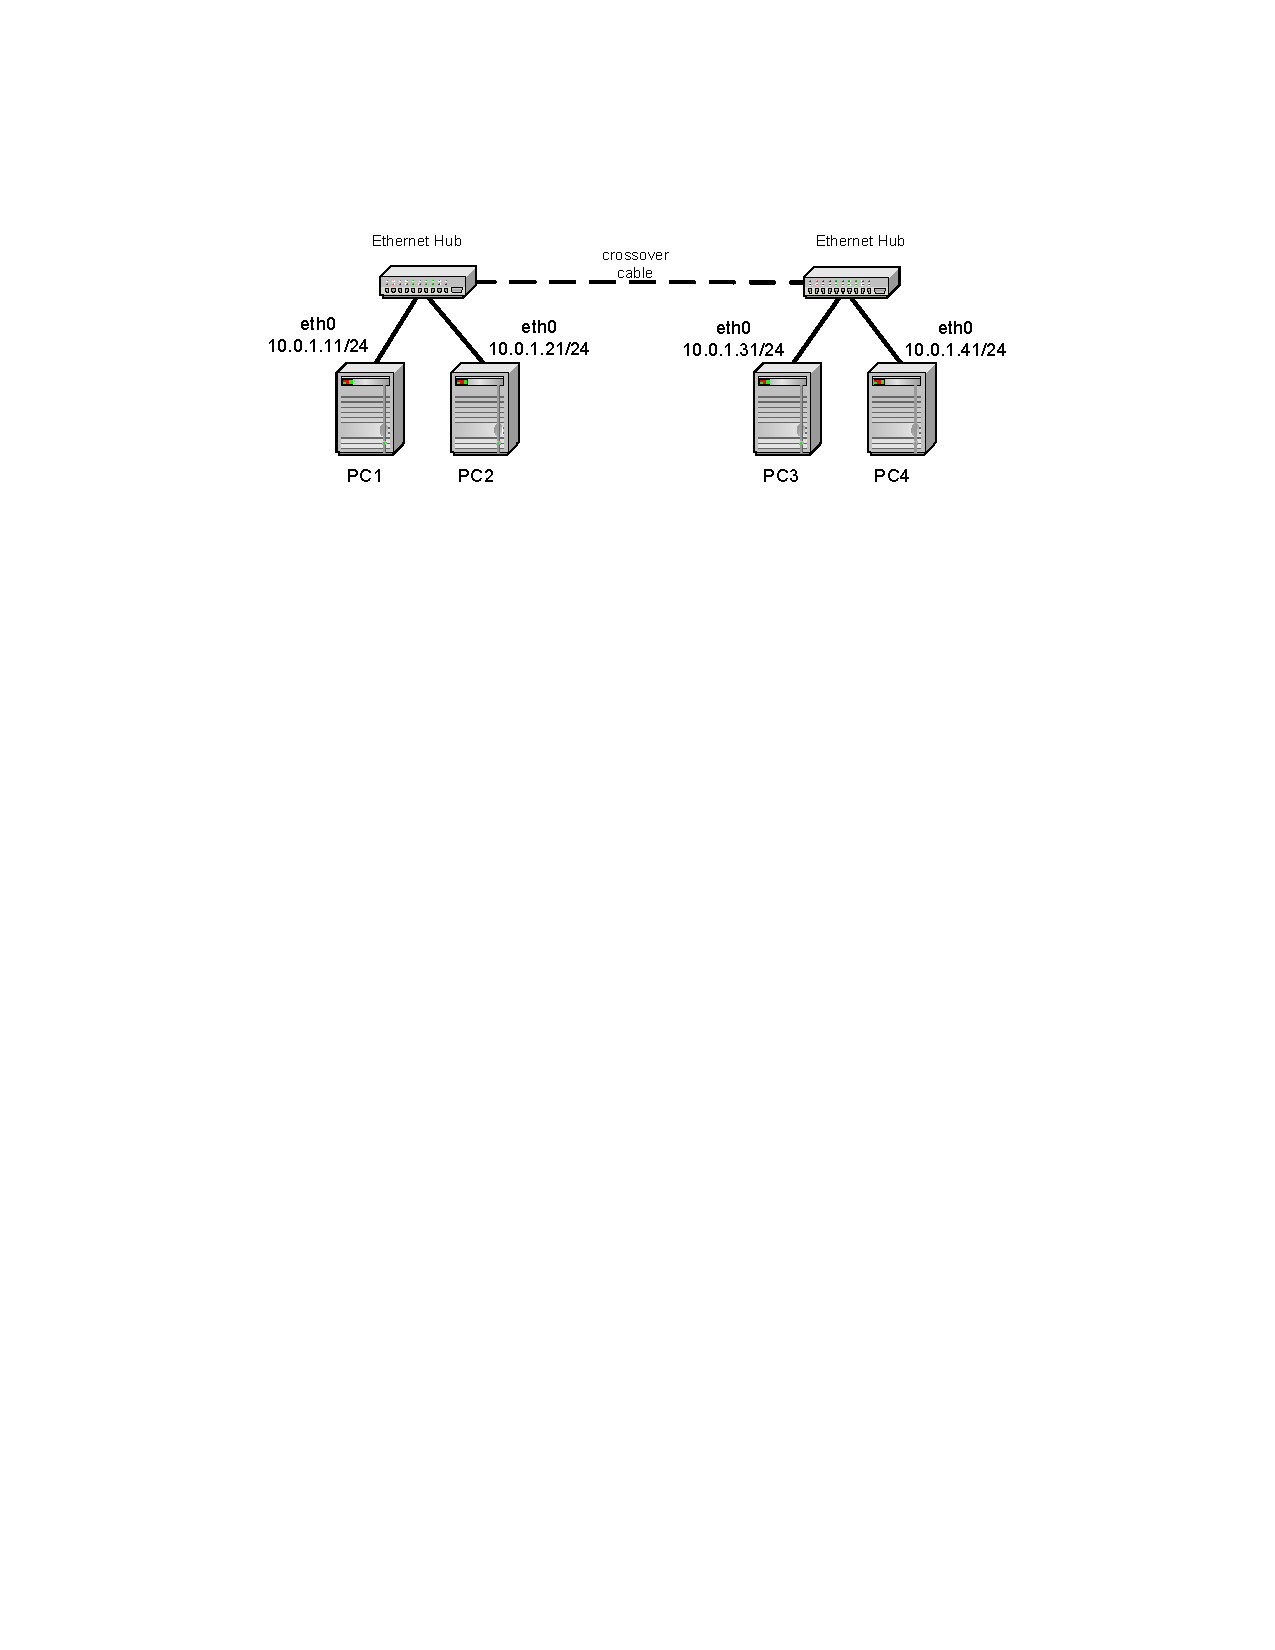
\includegraphics[width=\linewidth]{graphics/lab6-network3.pdf}	
	\caption{Network Topology for Part 3}
	\label{fig:lab6-network3}
\end{figure}

\begin{enumerate}
	\item Configure the network as shown in Figure \ref{fig:lab6-network3}. Starting from the network configuration from Part 2 (in Figure \ref{fig:lab6-network2}), disconnect Router1 and connect the two hubs directly with a crossover Ethernet cable (black cable, red RJ45 plugs).
	\item Determine the number of collisions on interface \iface{eth0} of PC1 and PC3, that have occurred since the PCs have been rebooted the last time, by typing
		\begin{cmdblock}
	PC1% ifconfig -a
	PC3% ifconfig -a
		\end{cmdblock}
		Save the output.
	\item Flood the network by generating a large number of ICMP Echo Request and Reply packets between PC1 and PC2, by typing
		\begin{cmdblock}
	PC1% ping -f 10.0.1.21
		\end{cmdblock}
	\item While the above ping command is running, start sending 100 ICMP Echo Request packets from PC3 to PC4.
		\begin{cmdblock}
	PC3% ping -c 100 10.0.1.41
		\end{cmdblock}
		Hopefully, these ping messages cause some collisions at the Ethernet hub.
	\item On PC1 and PC3, save the output of \cmd{ifconfig -a} again. Observe the number of new collisions that the above experiment has generated.
\end{enumerate}

\begin{questions}
	\q{3.A}{Calculate the number of new collision as seen by PC1 and PC3, in the above exercise. Briefly explain what causes the collisions.}
\end{questions}	

\subsubsection{Exercise 3-b. No collisions when using an Ethernet switch}
Repeat the steps of the previous exercise, but place an Ethernet switch (Router1, which has been configured as a bridge), between the two Ethernet hubs.

\begin{enumerate}
	\item Reconstitute the network configuration shown in Figure \ref{fig:lab6-network2}, by connecting Router1 between the two hubs.
	\item Obtain the number of collisions that have been observed on interface \iface{eth0} of PC1 and PC3 by typing
		\begin{cmdblock}
	PC1% ifconfig -a
	PC3% ifconfig -a
		\end{cmdblock}
		Save the output.
	\item Flood the network with traffic by generating a large number of ICMP Echo Request and Reply packets between PC1 to PC2, by typing 
		\begin{cmdblock}
	PC1% ping -f 10.0.1.21
		\end{cmdblock}
	\item Now issue 100 ICMP Echo Request packets from PC3 to PC4: 
		\begin{cmdblock}
	PC3% ping -c 100 10.0.1.41
		\end{cmdblock}
	\item Once again, save the output of the command \cmd{ifconfig -a} on PC1 and PC3, and record the number of collisions on interface \iface{eth0}.
	\item Access Router1 and run the \cmd{show bridge} command to display the bridge forwarding table. Save the data.
\end{enumerate}

\begin{questions}
	\q{3.B}{Use the \cmd{ifconfig -a} output to calculate the new collisions seen at the interfaces of PC1 and PC3. Explain the differences between the outcomes in Exercise 3-a and Exercise 3-b.}
\end{questions}
	
\newpage
\subsection{Learning Bridges}

Each bridge has a MAC forwarding table that determines the port where a packet is transmitted from. When a packet arrives, the bridge looks up the destination MAC address of the packet in its MAC forwarding table, and retrieves the outgoing port for this packet. If the destination MAC address is not found in the forwarding table, the bridge floods the packet on all ports, with exception of the port where the packet arrived.

Bridges update their MAC forwarding table using what is called a learning algorithm, which works as follows. A bridge examines the source MAC address of each packet that arrives on a particular port, and memorizes that the source address is reachable via that port. This is done by adding the source MAC address and the port to the MAC forwarding table. The next time the bridge receives a packet which has this MAC address as destination, the bridge finds the outgoing port in its forwarding table. Bridges that run this algorithm are referred to as learning bridges. All currently deployed Ethernet switches execute the learning algorithm.

An entry in the MAC forwarding table is deleted if it is not used (looked up) for a certain amount of time. The maximum time that a MAC address can stay in the forwarding table without a lookup is determined by the \emph{Ageing} value, which is a configuration parameter.

Here you investigate the learning algorithm of bridges. The network configuration is as shown in Figure \ref{fig:lab6-network4}.

\begin{figure}[h!t]
	\centering
	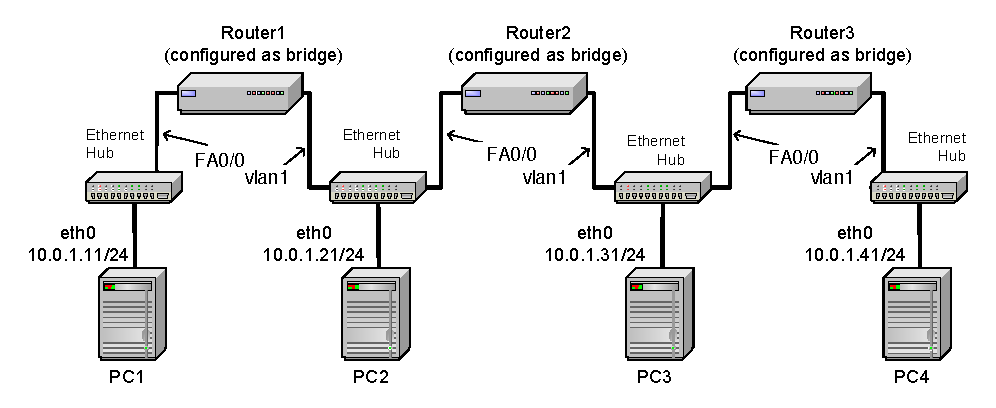
\includegraphics[width=\linewidth]{graphics/lab6-network4-updated.pdf}	
	\caption{Network Topology for Part 4}
	\label{fig:lab6-network4}
\end{figure}

\subsubsection{Exercise 4-a. Exploring the learning algorithm of bridges}

In this exercise you study how bridges set up their MAC forwarding tables from the network traffic.
\begin{enumerate}
	\item Set up the network configuration as shown in Figure \ref{fig:lab6-network4}.
	\item Establish a \cmd{minicom} session to Router1, Router2, and Router3.
		\begin{itemize}
			\item Configure Router1, Router2, and Router3 as bridges (Disable the spanning tree protocol).
			\item On each of the bridges, delete the contents of the MAC forwarding table with the \cmd{clear bridge} command.
		\end{itemize}
	\item Verify that PC2 is not running as a bridge. If necessary, follow the instructions in Exercise 1-d to disable the bridging functions on PC2. Also, verify that on each PC only interface \iface{eth0} is enabled.
	\item Start to capture traffic with ethereal on the \iface{eth0} interfaces of PC1, PC2, PC3, and PC4.
	\item Clear the ARP cache on PC1, PC2, and PC3.
	\item Now, issue a set of \cmd{ping} commands. After each command, save the MAC forwarding table on all bridges with the command show bridge, and observe how far the ICMP Echo Request and Reply packets travel.
		\begin{cmdblock}
	PC1% ping -c 1 10.0.1.21 
	PC2% ping -c 1 10.0.1.11 
	PC2% ping -c 1 10.0.1.41 
	PC3% ping -c 1 10.0.1.21
		\end{cmdblock}
	\item Stop the traffic capture on the PCs, and save the ethereal output.
\end{enumerate}

\begin{questions}
	\q{4.A.1}{ Use the captured data to illustrate the algorithm used by bridges to forward packets.}
	\q{4.A.2}{For each of the transmitted packets, explain if the learning algorithm results in changes to the MAC forwarding table. Describe the changes.}
\end{questions}

\subsubsection{Exercise 4-b. Learning about new locations of hosts}

Learning bridges adapt their MAC forwarding tables automatically when the location of a host changes. Due to the learning algorithm, the time it takes to adapt to a change depends on the network traffic and on the value of the Ageing parameter. This is illustrated in the following exercise.

\begin{enumerate}
	\item Continue with the configuration of the previous exercise. First, create or refresh entries in the MAC forwarding table at the bridges by issuing the following commands from PC1:
		\begin{cmdblock}
	PC1% ping -c 3 10.0.1.31 
	PC1% ping -c 3 10.0.1.41
		\end{cmdblock}
	\item Now, connect PC2 to the same hub that PC4 is connected to.
	\item Issue a ping command from PC1 that continuously sends ICMP Echo Request packets to PC2
		\begin{cmdblock}
	PC1% ping 10.0.1.21
		\end{cmdblock}
		Since Router2 does not know that PC2 has moved, it does not forward the ICMP Echo Request packet, and packet does not reach PC2. As a result, the ARP requests and the ping are unsuccessful. Eventually, since the MAC forwarding entry for PC2 is not refreshed at Router2 and Router3, the entry is deleted. When the entry is removed, the next ICMP Echo Request from PC1 is flooded on all ports, thus reaching PC2. When PC2 responds, all bridges update their MAC forwarding table using the source MAC address of PC2.
		Record the amount of time that the ping from PC1 to PC2 is not successful after PC2 has been moved to a different hub.
	\item Now connect PC3 to the same hub as PC4.
	\item Issue a \cmd{ping} command from PC1 to PC3 that continuously sends ICMP Echo Request packets to PC3: 
		\begin{cmdblock}
	PC1% ping 10.0.1.31
		\end{cmdblock}
	\item Then, generate a single ICMP Echo Request packet from PC3 to PC1 with the command
		\begin{cmdblock}
	PC3% ping -c 1 10.0.1.11
		\end{cmdblock}
		Now, if you look on PC1, you notice that the \cmd{ping} command is successful again. Explain this outcome and compare it to the outcome of Step 2.
\end{enumerate}

\begin{questions}
	\q{4.B.1}{Include the times that you recorded in Steps 3.}
	\q{4.B.2}{Explain the outcome of Step 6. That is, explain why the ping issued by PC3 has the effect that the ping commands from PC1 to PC3 (in Step 5) are successful. Compare the outcome with the outcome in Step 3.}
\end{questions}

\setcounter {chapter} {6}
%!TEX root = labo.tex

\setcounter {chapter} {6} 

\chapter{Network Address Translation (NAT)\\Dynamic Host Configuration Protocol (DHCP)}

What you will learn in this lab:
\begin{itemize}
	\item How NAT (Network Address Translation) works.
	\item How DHCP (Dynamic Host Configuration Protocol) works.
	\item How DHCP works together with NAT.
\end{itemize}

\newpage
\setsession{prelab7}
\section{Prelab 7}\label{sec:prelab7}
%!TEX root = labo.tex

\subsubsection*{NAT and DHCP}
Use the following resources to prepare yourself for this lab session:
\begin{enumerate}
	\item Unix commands for NAT, DHCP: Go to the online manual pages at \url{http://manpages.ubuntu.com/}. Read the manual pages of the following commands for the operating system version "trusty 14.04 LTS":
		\begin{itemize}
			\item iptables
			\item dhclient
			\item dhcpd
			\item dhcpd.conf
			\item dhcp-options
			\item dhcpd.leases
		\end{itemize}
	\item Private IP addresses: Read RFC 1918 on address allocation in private networks \url{http://tools.ietf.org/html/rfc1918}.
	\item Network Address Translation (NAT): Read the following tutorial on NAT at \url{http://www.firewall.cx/networking-topics/network-address-translation-nat.html}.
	\item Netfilter/iptables Read about netfilter and iptables at \url{http://www.netfilter.org} and \url{http://www.thegeekstuff.com/2011/01/iptables-fundamentals/}.
	\item Dynamic Host Configuration Protocol (DHCP): Read RFC 2131 on DHCP at \url{http://tools.ietf.org/html/rfc2131}.
\end{enumerate}

\newpage
\subsection*{Prelab Questions}
\begin{questions}
	\q{1}{Explain why NAT is often mentioned as a solution to counteract the depletion of IP addresses on the global Internet? Which alternatives to NAT exist that address the scarcity of available IP addresses?}
	\q{2}{What does the following comment refer to: ``NAT destroys the ability to do host-to-host communication over the Internet``?}
\end{questions}

Explain the following terms which are used in the context of Network Address Translation:
\begin{questions}
	\q{3.a}{Static NAT}
	\q{3.b}{Dynamic NAT}
	\q{3.c}{NAT with IP overload}
	\q{3.d}{Port Address Translations e.g. IP Masquerading}
	\q{4}{Refer to RFC 1918 and list the IP address blocks that are reserved for use in private networks. Why is there a need to specify IP addresses for private networks?}	
	\q{5}{The utility netfilter and the command iptables provide support for NAT in Linux systems. Explain the relationship between the netfilter utility and the iptables command?}
\end{questions}

Describe the following terms which are used in the iptables command:
\begin{questions}
	\q{6.a}{Chain}
	\q{6.b}{Postrouting }
	\q{6.c}{Prerouting}
\end{questions}

Consider a NAT device between a private and the public network. Suppose the private network uses addresses in the range 10.0.1.0-10.0.1.255, and suppose that the interface of the NAT device to the public network has IP address 128.143.136.80.
\begin{questions}
	\q{7.a}{Write the iptables command so that the addresses in the private network are mapped to the public IP address 128.143.136.80.}
	\q{7.b}{Write an IOS command so that the addresses in the private network are mapped to the public IP address 128.143.136.80.}
\end{questions}

Answer the following questions about DHCP:
\begin{questions}
	\q{8}{Explain the meaning of the ``magic cookie'' in the DHCP protocol.}
	\q{9}{If the command \cmd{dhcpd} is issued (without arguments) on a Linux PC with multiple network interfaces, which network interfaces does the DHCP server listen on?}
\end{questions}


\newpage
\setsession{lab7}
\section{Lab 7}\label{sec:lab7}

Figure \ref{fig:lab7-part1-network} shows two private networks which are connected to a public network. Each private network is connected to the public network by a NAT device, which is either a PC or a Cisco router. On each NAT device, IP forwarding must be enabled.

\boxwarning{In the private networks in Figure \ref{fig:lab7-part1-network}, Router1 and Router3 are used to mimic hosts, i.e., they are not configured to act as IP routers.)}

\begin{figure}[ht]
	\centering
	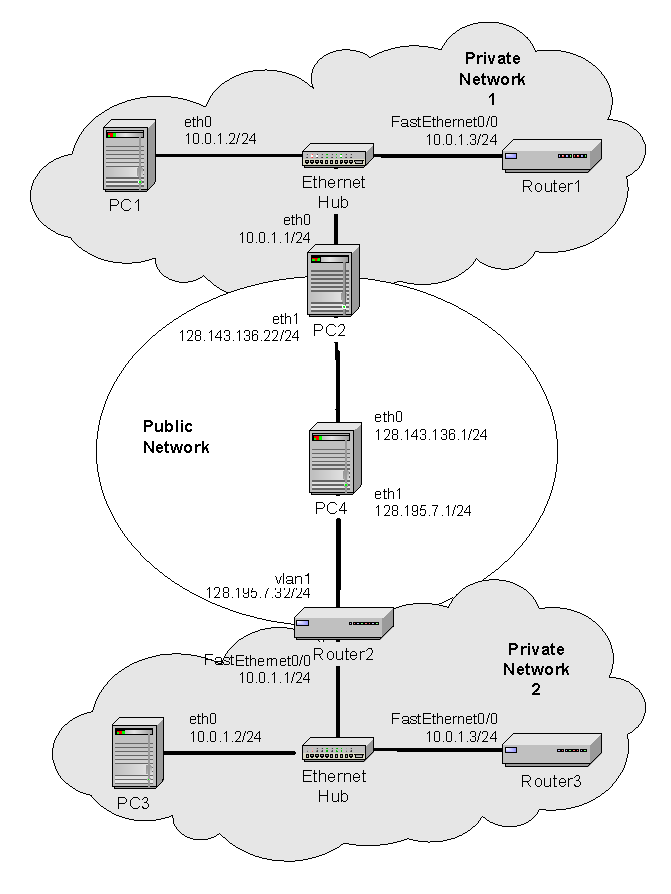
\includegraphics{graphics/lab7-part1-updated.pdf}	
	\caption{Network configuration for Part 1.}
	\label{fig:lab7-part1-network}
\end{figure}

\begin{table}[h!t]
	\centering
	\begin{tabular}{| c | c | c | c |}	
		\hline
		\textbf{Linux PC} & \textbf{IP Addresses of eth0} & \textbf{IP Addresses of eth1} & \textbf{Default Gateway} \\ \hline
		PC1 & 10.0.1.2/24 & none & 10.0.1.1 \\ 
		PC2 & 10.0.1.1/24 & 128.143.136.22/24 & 128.143.136.1 \\
		PC3 & 10.0.1.2/24 & none & 10.0.1.1 \\
		PC3 & 128.143.136.1/24 & 128.195.7.1/24 & none \\ \hline
	\end{tabular}
	\caption{IP addresses and gateways assignment of all PCs for Part 1.}
	\label{tab:lab7-part1-ip-addresses-pc}
\end{table}

\begin{itemize}
	\item In this lab, PC2 and Router2 are routers that provide the gateways between the private and the public networks. Both PC2 and Router2 are configured as NAT devices.
	\item On PC2, the kernel is built with netfilter, an extension to the Linux kernel that provides the kernel with the ability to set IP packet filters, including NAT functions. On Router2, you will use Cisco IOS commands to configure NAT rules.
	\item PC4 runs as an IP router. (We use a Linux PC instead of a Cisco Router so that wireshark can be used to capture traffic on the public network).
	\item The assignment of IP addresses and default gateways for all PCs and routers are shown in Table1 and Table 2.
	\item The console port of Router1 is connected to a serial port of PC1, the console port of Router2 is connected to a serial port of PC2, and the console port of Router3 is connected to a serial port of PC3.
\end{itemize}

\begin{table}[h!t]
	\centering
	\begin{tabular}{| c | c | c | c | c |}	
		\hline
		\textbf{Linux PC} & \textbf{IP Addresses of FA0/0} & \textbf{IP Addresses of vlan1} & \textbf{Default Gateway} & \textbf{Connected PC} \\ \hline
		Router1 & 10.0.1.3/24 & none & 10.0.1.1 & PC1 \\ 
		Router2 & 10.0.1.1/24 & 128.195.7.32/24 & 128.195.7.1 & PC2 \\
		Router3 & 10.0.1.3/24 & none & 10.0.1.1 & PC3\\ \hline
	\end{tabular}
	\caption{IP addresses and gateways assignment of all routers for Part1.}
	\label{tab:lab7-part1-ip-addresses-routers}
\end{table}

\newpage
\subsection{NAT (Network Address Translation)}

NAT (Network Address Translation) refers to a function that replaces the IP addresses (and possibly the port numbers) of IP datagrams. NAT is run on routers that connect private networks to the public Internet, to replace the IP address-port pair of an IP packet with another IP address-port pair. Generally, the operations of NAT are specified in terms of a set of rules which determines how IP addresses are to be replaced.

Often, a NAT device is referred to as a NAT box. One of the reasons for using NAT is that it conserves IP addresses. NAT allows hosts in a private network to share public IP addresses, or to limit the use of public IP addresses to a small number of hosts in the private network.

Private networks may have IP addresses that are non-Internet routable, as specified in RFC 1918. This means that the Internet routers do not have entries in their routing tables for these addresses.

In the network in Figure \ref{fig:lab7-part1-network}, both PC2 and Router2 will be configured as NAT devices. With NAT, the hosts in the private networks can access the public network, i.e., they are able to reach the addresses on the 128.143.136.0/24 and 128.195.7.0/24 networks.

\subsubsection{Exercise 1-a: Network Setup}
Configure the network in Figure \ref{fig:lab7-part1-network} with the IP address configuration shown in Table \ref{tab:lab7-part1-ip-addresses-pc} and Table \ref{tab:lab7-part1-ip-addresses-routers}. The following commands review the steps involved in the configuration.
\begin{enumerate}
	\item On the Linux PCs, use \cmd{ifconfig} to configure the IP address of the interfaces. Add a default gateway on each PC with the command (shown for PC1):
		\begin{cmdblock}
	PC1% route add default gw gateway_address
	\end{cmdblock}
	\item IP forwarding must be enabled on PC2 and PC4.
	\item Use a serial cable to connect a serial port of a PC to the console port of a router. Use the \cmd{minicom} command to access the routers.
	\item Configure the IP addresses of interfaces \iface{Fa/0} and \iface{vlan1} on the routers, and set the default gateways as shown in Table \ref{tab:lab7-part1-ip-addresses-routers}. Below is the sample configuration for Router2.
		\begin{cmdblock}
	Router2> enable
	Password: <enable secret>
	Router2# configure terminal
	Router2(config)# no ip routing
	Router2(config)# ip routing
	Router2(config)#ip route 0.0.0.0 0.0.0.0 128.195.7.1
	Router2(config)# interface FastEthernet0/0 
	Router2(config-if)# no shutdown
	Router2(config-if)# ip address 10.0.1.1 255.255.255.0 
	Router2(config-if)# interface FastEthernet0/1 
	Router2(config-if)# no shutdown
	Router2(config-if)# interface vlan1 
	Router2(config-if)# no shutdown
	Router2(config-if)# ip address 128.195.7.32 255.255.255.0
	Router2(config-if)# end
		\end{cmdblock}
		The following commands sets 128.195.7.1 as the default gateway of Router2.
		\begin{cmdblock}
	Router2(config)# ip route 0.0.0.0 0.0.0.0 128.195.7.1
		\end{cmdblock}
\end{enumerate}

After completing the set up of the configuration you should be able to issue successful intra network ping commands i.e., between hosts in the private network, and between hosts in the public network. However, ping commands across a private/public network boundary are not successful.

\subsubsection{Exercise 1-b: Configuration of NAT on a Cisco Router}
\boxwarning{You will use Wireshark in this exercise. Do not forget to append the binary dump (pcap format) to your lab report}
A Cisco router can be set up to run as a NAT device.

\boxinfo {In Cisco IOS, the private network is referred to as ``inside'' and the public network is referred to as ``outside''. An IP address that is seen by hosts on the inside is called a local address, and an IP address that is seen by hosts on the outside is called a global address. There are four different types of addresses:
\begin{itemize}
	\item An inside local address is an address in the private network that is not visible in the public network.
	\item An inside global address can be used in the public network for devices in the private network.
	\item An outside global address is an address in the public network that is not made known in the private network.
	\item An outside local address is used by devices in the private network to addresses in the public network.
\end{itemize}
Using this terminology, a NAT device translates inside local addresses to outside global addresses and outside global addresses to inside local addresses.
}

\begin{enumerate}
	\item Modify the NAT table of Router2: Use the following commands to set up Router2 as a NAT device.
		\begin{itemize}
			\item A NAT rule is added so that the private IP address of PC3, 10.0.1.2, is translated to the public address 200.0.0.2.
				The IOS commands are as follows:
				\begin{cmdblock}
	Router2> enable
	Password: <enable secret>
	Router2# show ip nat translations
	Router2# configure terminal
	Router2(config)# interface FastEthernet0/0
	Router2(config-if)# ip nat inside
	Router2(config-if)# interface vlan1
	Router2(config-if)# ip nat outside
	Router2(config-if)# exit
	Router2(config)# ip nat inside source static 10.0.1.2 200.0.0.2 
	Router2(config)# end
	Router2# show ip nat translations
				\end{cmdblock}
			\item After the above rule has been entered, display the content of the NAT table and save it to a file.
				The commands used above are explained below:
				\begin{itemize}
					\item Displays the content of the NAT table:
						\begin{cmdblock}
	Router2# show ip nat translations
						\end{cmdblock}
					\item Specifies that interface \iface{FastEthernet0/0} is connected to the private network.
						\begin{cmdblock}
	Router2(config)# interface FastEthernet0/0
	Router2(config-if)# ip nat inside
						\end{cmdblock}
					\item Specifies that interface \iface{vlan1} is connected to the public network.
						\begin{cmdblock}
	Router2(config-if) #interface vlan1
	Router2(config-if)# ip nat outside
						\end{cmdblock}
					\item Adds a rule so that the private address 10.0.1.2 is mapped to the public address 200.0.0.2
						\begin{cmdblock}
	Router2(config)# ip nat inside source static 10.0.1.2 200.0.0.2
						\end{cmdblock}
				\end{itemize}
			\end{itemize}
		\boxinfo {``Dynamic NAT'' is an alternative to the static NAT table entries used in this exercise. With dynamic NAT, a pool of global addresses is specified at the NAT device. Addresses from the pool are dynamically mapped to the private addresses whenever there is a demand for a new address.}
	\item Update routing tables: Add static routing entries to the routing table of PC4, so that traffic with destination IP address 200.0.0.0/24 is forwarded to Router2.
	\item Observe traffic at a NAT device: To observe the IP address translation, issue ping commands between machines in the public and private network. Use Wireshark to capture packets on the private and public interfaces of Router2.
		\begin{itemize}	
			\item Start an Wireshark session on PC3 to capture the traffic from Router2 on the private network.
			\item Start an Wireshark session on interface \iface{eth1} of PC4 to capture the traffic from Router2 on the public network.
			\item Issue the following ping commands: 
				On PC3:
				\begin{cmdblock}
	PC3% ping -c 3 10.0.1.3
	PC3% ping -c 3 128.143.136.1
				\end{cmdblock}
				On Router3:
				\begin{cmdblock}
	Router3# ping 10.0.1.2
	Router3# ping 128.143.136.1
				\end{cmdblock}
				On PC4:
				\begin{cmdblock}
	PC4% ping -c 3 10.0.1.2 
	PC4% ping -c 3 200.0.0.2
				\end{cmdblock}
			\item Save the Wireshark data to files. Observe which ping commands succeed.
		\end{itemize}
	\item Add additional NAT table entries: Add NAT rules to Router2, so that Router2 and Router3 (on interface \iface{Etherenet0/0}) are addressable from the public network. The private and public addresses are given in Table \ref{tab:lab7-nat-router2-router3}.
		\begin{table}[h!t]
			\centering
			\begin{tabular}{| c | c | c |}	
				\hline
				\textbf{Linux PC} & \textbf{Inside local address} & \textbf{Outside local address}  \\ \hline
				Router2 & 10.0.1.1/24 & 200.0.0.1 \\ 
				Router3 & 10.0.1.3/24 & 200.0.0.3 \\ \hline
			\end{tabular}
			\caption{Private and public addresses of Router2 and Router3.}
			\label{tab:lab7-nat-router2-router3}
		\end{table}
\end {enumerate}

\begin{questions}
	\q{1.B.a}{Include the NAT table of Router2 and provide an explanation of the columns of the table.}
	\q{1.B.b}{For each of the ping commands above, provide an explanation why the command succeeds or fails.}
	\q{1.B.c}{Include the IP source address and IP destination address from the IP header data of an ICMP request and the corresponding ICMP reply packet before and after it passes through Router2.}
\end{questions}
	
\subsubsection{Exercise 1-c: IP Masquerading with a Linux PC}
\boxwarning{You will use Wireshark in this exercise. Do not forget to append the binary dump (pcap format) to your lab report}
In this exercise, we consider a special use of NAT that allows multiple private IP addresses to be mapped to a single public IP address. This use of NAT is called IP masquerading, port address translation (PAT) or Network Address and Port Translation (NAPT). Here, the private network has only a single public IP address, but has multiple hosts in the private network. IP Masquerading modifies the port number of packets so that the single public IP address can be overloaded.

In this exercise, PC2 will be configured to perform IP masquerading. The Linux kernel on all PCs has been built with netfilter, which adds the ability to set IP packet filters in a Linux system. IP packet filters are used to add firewalls as well as NAT functionality to a system. The \cmd{iptables} command is used to set up, maintain, and inspect IP packet filter rules to a Linux kernel.

\boxinfo {On a Linux system, the configuration of NAT manipulates a set of rules of the netfilter utility, called NAT table. The rules in the NAT table are grouped in so- called chains. Two of the built-in chains are called \texttt{PREROUTING} and \texttt{POSTROUTING}:
	\begin{description}
		\item[\texttt{PREROUTING}] \hfill \\
			The rules in this chain are applied to incoming datagrams.
		\item[\texttt{POSTROUTING}] \hfill \\
			The rules in this chain are applied to outgoing datagrams. The main rule is SNAT (Source Network Address Translation), which specifies how the source address of an outgoing IP datagram should be modified.
	\end{description}
}

Commands that manipulate the NAT table start with
\begin{cmdblock}
	PC2% iptables -t nat
\end{cmdblock}

\boxinfo {The following are some of the most important commands that manipulate the NAT table:
	\begin{description}
		\item[\texttt{iptables -t nat -L}] \hfill \\
			Displays all rules in the NAT table
		\item[\texttt{iptables -t nat -L}] \hfill \\
			Deletes the first rule in the \texttt{POSTROUTING} chain of the NAT table
		\item[\texttt{iptables -t nat -F}] \hfill \\
			Deletes all entries in (``flushes'') the NAT table
		\item[\texttt{iptables -t nat -A POSTROUTING -j SNAT -{}-to IPAddr -s PrivateIPAddr/netmask}] \hfill \\
			Adds the following rule to the \texttt{POSTROUTING} chain of the NAT table: ``In IP datagrams that go to the public network, the IP source address PrivateIPAddr/netmask is changed to IPAddr''.\\
			Example: The source address of outgoing IP datagrams that match ``10.0.1.0/24'' is changed to 128.195.7.32.\\
			\cmd{iptables -t nat -A POSTROUTING -j SNAT -{}-to 128.195.7.32 -s 10.0.1.0/24}
	\end{description}
}

\begin{enumerate}
	\item Modify the NAT table of PC2: On PC2, add a rule to the NAT table so that the IP source address of all outgoing IP datagrams are set to IP address 128.143.136.22. Display the content of the NAT table and save it to a file.
	\item Observe traffic at a NAT device:
		\begin{itemize}
			\item To observe the IP address translation, capture packets on both interfaces of PC2 that are between the private networks and the Internet. On PC2, run Wireshark on both \iface{eth0} and \iface{eth1}.
			\item Establish a set of Telnet session and login to remote machines, using the following \cmd{telnet} commands:
				On PC1:
				\begin{cmdblock}
	PC1% telnet 10.0.1.3
	PC1% telnet 128.143.136.1
				\end{cmdblock}
				On Router1:
				\begin{cmdblock}
	Router1# telnet 10.0.1.2
	Router1# telnet 128.143.136.1
				\end{cmdblock}
				On PC4:
				\begin{cmdblock}
	PC4% telnet 10.0.1.2
				\end{cmdblock}
			\item Save the Wireshark data to files. Observe which Telnet commands succeed.
			\item For the successful Telnet sessions, observe how the IP addresses and port numbers are mapped.
		\end{itemize}
	\item Observe mapping of ICMP packets: The ping command sends out ICMP Echo Request messages and receives ICMP Echo Reply messages. Since ICMP messages do not contain a port number, it is not entirely obvious how a NAT device that performs IP masquerading can direct ICMP Echo Reply messages that return from the public network to the private network. In this exercise, you will explore how a NAT device handles ICMP messages.
		\begin{itemize}
			\item On PC2, run Wireshark on both \iface{eth0} and \iface{eth1}. Use the appropriate filters to capture the traffic generated by ping commands.
			\item Issue the following ping commands:
				On PC1:
				\begin{cmdblock}
	PC1% ping -c 3 10.0.1.3
	PC1% ping -c 3 128.143.136.1
				\end{cmdblock}
				On Router1:
				\begin{cmdblock}
	Router1# ping 10.0.1.2
	Router1# ping 128.143.136.1
				\end{cmdblock}
				On PC4:
				\begin{cmdblock}
	PC4% ping -c 3 10.0.1.2
				\end{cmdblock}
			\item Save the Wireshark output and the output of ping commands into files.
		\end{itemize}
\end{enumerate}

\begin{questions}
	\q{1.C.a}{For each of the \cmd{telnet} and \cmd{ping} commands above, provide an explanation why a command succeeds or fails.}
	\q{1.C.b}{For each successful telnet session, include the IP header data of an outgoing and an incoming packet header (with respect to the private network).}
	\q{1.C.c}{For each successful ping command, include the IP header data of an outgoing ICMP Request message and an incoming ICMP reply message (with respect to the private network).}
	\q{1.C.d}{How does PC know that a packet coming from the public network is destined to a host in the private network?}
	\q{1.C.e}{Explain the steps performed by the kernel during IP address translation.}
\end{questions}

\subsubsection{Exercise 1-d: NAT and FTP}
\boxwarning{You will use Wireshark in this exercise. Do not forget to append the binary dump (pcap format) to your lab report}

NAT can create problems for applications, which carry the IP addresses in the payload of an IP datagram. An example of such an application is the file transfer program (FTP).

In this exercise, you establish an FTP connection from PC3 in the private network to PC2 in the public network, and observe how the FTP application works with NAT.

\begin{enumerate}
	\item Start Wireshark on interface \iface{eth0} of PC4 and on interface \iface{eth0} of PC3.
	\item FTP session between two hosts in the public network:
		\begin {itemize}
			\item Start the FTP server on PC2 by typing
				\begin{cmdblock}
	PC2% service vsftpd start
				\end{cmdblock}
			\item Start an FTP connection from PC4 to PC2 (the -d option prints out debug messages).
				\begin{cmdblock}
	PC4% cd /root/labdata
	PC4% ftp -d 128.143.136.22
				\end{cmdblock}
				Login with user name ``root'' and enter the root password.
			\item Download a file from the FTP server.
				\begin{cmdblock}
	ftp> get fname
				\end{cmdblock}
				where \path{fname} is a file on the remote server. (You can use the command ls to obtain a list of all files in the remote directory.)
			\item Use the traffic captured by Wireshark to determine where the payload of FTP data carries information on IP addresses.
			\item Save the Wireshark output and the FTP debug information output into files.
		\end{itemize}
	\item FTP session from a private to the public network:
		\begin{itemize}
			\item Use the same commands as previously to download a file from PC2 to PC3
				\begin{cmdblock}
	PC3% ftp -d 128.143.136.22
				\end{cmdblock}
				Is the FTP session establishment successful?
			\item Save the traffic captured by wireshark and save the FTP debug information output. Make sure that you save enough data to answer the lab report questions.
		\end{itemize}
\end{enumerate}

\begin{questions}
	\q{1.D.a}{Use the captured data to explain the outcome of the FTP experiment. In particular, if the file was successfully downloaded, explain how the problem of sending the IP address as part of the data payload of the IP packet is solved.}
	\q{1.D.b}{How can NAT be used to spoof a host address? How can you prevent this?}
\end{questions}

\newpage
\subsection{Dynamic Host Configuration Protocol (DHCP)}

The Dynamic Host Configuration Protocol (DHCP) can be used to dynamically set and change configuration parameters of Internet hosts, including IP address, subnet mask, default router, and DNS server. DHCP is based on a client-server model. DHCP clients send requests to a DHCP server and the server responds with an allocation of IP addresses and other configuration parameters.

In this part of the lab, you will also learn about DHCP relay agents. When the DHCP client and DHCP server are not on the same IP network, DHCP relay agents can act as routers of DHCP messages. A DHCP relay agent can forward DHCP requests from a DHCP client to a DHCP server and it can forward the reply messages from the DHCP server to the DHCP client.

The network configuration for Part 2 is shown in Figure \ref{fig:lab7-part2}. PC1, PC3, and PC4 are set up as DHCP clients, and initially do not have IP addresses. PC2 is configured as a DHCP server, which listens for DHCP requests on all of its interfaces and transmits network configuration parameters. Router1 acts as a DHCP relay agent, which forwards DHCP messages between different IP networks.

Table \ref{tab:lab7-part2-ip-addresses-pc} lists the range of addresses that are associated at the DHCP server PC2 with each IP network.

\begin{figure}[h!t]
	\centering
	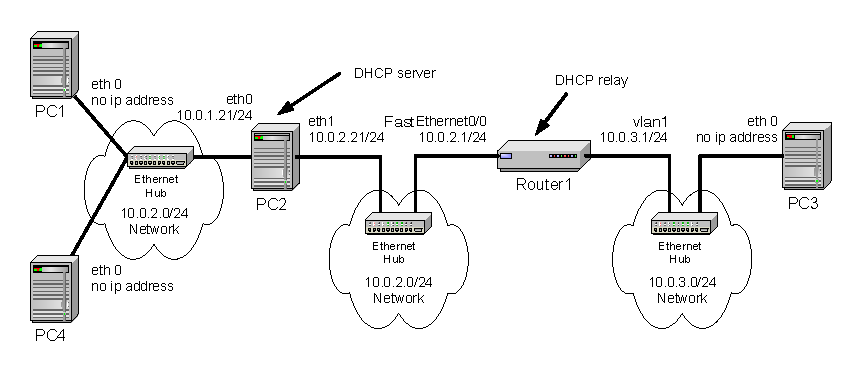
\includegraphics{graphics/lab7-part2-updated.pdf}	
	\caption{Network configuration for Part 2.}
	\label{fig:lab7-part2}
\end{figure}

\begin{table}[h!t]
	\centering
	\begin{tabular}{| c | c | c | c |}	
		\hline
		\textbf{Linux PC} & \textbf{IP Addresses of eth0} & \textbf{IP Addresses of eth1} & \textbf{Default Gateway} \\ \hline
		PC1 & none & none & none \\ 
		PC2 & 10.0.1.21/24 & 10.0.2.21/24 & 10.0.2.1 \\
		PC3 & none & none & none \\ 
		PC3 & none & none & none \\ \hline
	\end{tabular}
	\caption{Configuration of the PCs in Part 2.}
	\label{tab:lab7-part2-ip-addresses-pc}
\end{table}

\begin{table}[h!t]
	\centering
	\begin{tabular}{| c | c | c | c | c |}	
		\hline
		\textbf{Linux PC} & \textbf{IP Addresses of eth0} & \textbf{IP Addresses of eth1} & \textbf{Default Gateway} & \textbf{Connected PC} \\ \hline
Router1 & 10.0.2.1/24 & 10.0.3.1/24 & 10.0.2.21 & PC1 \\ \hline
	\end{tabular}
	\caption{Configuration of the Routers in Part 2.}
	\label{tab:lab7-part2-ip-addresses-routers}
\end{table}

\begin{table}[h!t]
	\centering
	\begin{tabular}{| c | c | c | c | c |}	
		\hline
		\textbf{Subnet} & \textbf{Range of Addresses} & \textbf{Default Router} \\ \hline
		10.0.1.0/24 & 10.0.1.2 to 10.0.1.10 & 10.0.1.21 \\ 
		10.0.3.0/24 & 10.0.3.2 to 10.0.3.10 & 10.0.3.1 \\ \hline
	\end{tabular}
	\caption{DHCP server configuration.}
	\label{tab:lab7-part2-dhcp}
\end{table}

\subsubsection{Exercise 2-a: Network Setup}
\begin{enumerate}
	\item We strongly recommend that you reboot the PCs and the routers before you proceed. Don't forget to save your files on a USB stick or online before rebooting.
	\item Set up the network topology as shown in Figure \ref{fig:lab7-part2}. Configure the IP addresses of the PCs and Router1 as shown in Table \ref{tab:lab7-part2-ip-addresses-pc} and Table {tab:lab7-part2-ip-addresses-routers}.
	\item It is important that PC1, PC3 and PC4 do not have a default route and do not have an IP address associated with their respective interface eth0.
\end{enumerate}

Review the routing table and the interface configuration. On PC1, this is done with the commands:

\begin{cmdblock}
	PC1% netstat -rn
	PC1% ifconfig -a
\end{cmdblock}

In Linux, routing tables display the default route as an entry with destination 0.0.0.0. If the routing table shows a default route, you can delete this and all other routing table entries by setting the IP address to 0.0.0.0. This is done with the following command:

\begin{cmdblock}
	PC1% ifconfig eth0 0.0.0.0 up
\end{cmdblock}

\subsubsection{Exercise 2-b: Configuring and starting a DHCP server}
On a Linux system, a DHCP server is started with the command \cmd{dhcpd}. The DHCP server reads the configuration file \path{/etc/dhcpd.conf}. The configuration file contains information on available IP addresses, and other configuration information. The following is an example of a configuration file for a DCHP server:

\begin{cmdblock}
	#dhcpd.conf file
	default-lease-time 600;

	subnet 10.0.1.0 netmask 255.255.255.0 {
		range 10.0.1.10 10.0.1.100; 
		option routers 10.0.1.1; 
		default-lease-time 120;
	}
	subnet 10.0.2.0 netmask 255.255.255.0 {
		range 10.0.2.101 10.0.2.200; 
	}

	subnet 10.0.3.0 netmask 255.255.255.0 { 
		range 10.0.3.6 10.0.3.10;
	}
\end{cmdblock}

The DHCP client is assigned an IP address for a period of time that is known as a lease. The above configuration file assigns IP addresses for a lease time of 600 seconds (default-lease- time). For requests on network 10.0.1.0/24, the DHCP server assigns IP addresses in the range 10.0.1.10 - 10.0.1.100, assigns 10.0.1.1 as the default gateway, and limits the lease of addresses to 120 seconds, thus, overruling the global limit of 600 seconds. For requests on network 10.0.2.0/24, the server assigns IP addresses in the range 10.0.2.101- 10.0.2.200.

\begin{enumerate}
	\item Set the DHCP configuration file: On PC2, set up the configuration file so that IP addresses are assigned as follows. On network 10.0.1.0/24, IP addresses are assigned in the range 10.0.1.2-10.0.1.10 with default gateway 10.0.1.21. On network 10.0.3.0/24, IP addresses are assigned in the range 10.0.3.2-10.0.3.10 with default gateway 10.0.3.1.
Note that these assignments are similar to, but not identical with the configuration file shown above.
	\item Start the DHCP server: On PC2, start the DHCP server by typing 
		\begin{cmdblock}
	PC2% dhcpd
		\end{cmdblock}
		The DHCP server daemon listens for requests from DHCP clients on all its interfaces. In Linux, the DHCP server must be restarted each time the configuration file is modified. Since only one DHCP server can run at a time, you may need to terminate the current DHCP server process.
\end{enumerate}

\subsubsection{Exercise 2-c: Starting a DHCP client}
\boxwarning{You will use Wireshark in this exercise. Do not forget to append the binary dump (pcap format) to your lab report}

The following steps start a DHCP client on PC1.
\begin{enumerate}
	\item On PC1, perform the following functions:
		\begin{itemize}
			\item Ensure that no default router entry exists in the routing table.
			\item A Linux DHCP client caches information from previous uses of DHCP. The cached information is stored in :
				\begin{cmdblock}
	/var/lib/dhcp3/
				\end{cmdblock}
				Since this cached information may interfere with your work, delete the lease files related to dhclient, if they exist:
				\begin{cmdblock}
	rm /var/lib/dhcp3/dhclient*
				\end{cmdblock}
			\item Start Wireshark on interface \iface{eth0} of PC2. (Set the display filter to ``bootp.dhcp'' so that only DHCP traffic is displayed in the window.)
		\end{itemize}
	\item Start a DHCP client with the command
		\begin{cmdblock}
	PC1% dhclient eth0
		\end{cmdblock}
\end{enumerate}

Save the data that is captured by Wireshark to a file. Save enough data to answer the following questions from the captured traffic:

\begin{questions}
	\q{2.C.2.a}{Which IP address is assigned to PC1?}
	\q{2.C.2.b}{	Observe the source and destination IP addresses of the packets that are sent between DHCP client and DHCP server.}
	\q{2.C.2.c}{How is it possible that a host can send and receive DHCP packets, even though it does not have an IP address?}
	\q{2.C.2.d}{Do you observe any ARP packets? If so, explain the function of the ARP in this context.}
	\q{2.C.2.e}{Observe and interpret the output of the DHCP packets. You should see the following packet types: DHCP Discover, DHCP Offer, DHCP Request, DHCP ACK.}
	\q{2.C.2.f}{Identify and interpret all option fields in the DHCP packet types that you observe.}
\end{questions}

\begin{enumerate}
	\item Renewing leases of IP addresses: The DHCP client is assigned an IP address for a limited period of time, which is called a lease. The maximum time of a lease is specified in the \path{dhcpd.conf} file. Information on current leases is stored at both the client side and the server side.
		\begin{itemize}
			\item In Linux, information on the current leases is stored in the following files \path{/etc/dhcpd.leases} at the DHCP server and \path{/var/lib/dhcp3/dhclient-eth0.lease} at the DHCP client (note that the latter name may differ).
			\item To interpret the content of the files, refer to the manual pages of dhcpd.conf, dhcp-options, and dhcpd.leases.
			\item Save the files that contain the information on current leases.
			\item Observe how a DHCP client renews a lease and save the captured traffic to a file.
				\begin{itemize}
					\item What type of DHCP message can be observed?
					\item How long does a DHCP client wait until it attempts to renew its lease?
				\end{itemize}
			\item Stop the process that runs the DHCP server by terminating the process \cmd{dhcpd} with the command
				\begin{cmdblock}
	PC2% pkill dhcpd
				\end{cmdblock}
				Observe what the DHCP client does when it cannot reach the DHCP server. Use the command \cmd{ifconfig -a} to see how long the DHCP client waits until it releases the leased IP address.
			\item Restart the DHCP server process by typing
				\begin{cmdblock}
	PC2% dhcpd
				\end{cmdblock}
		\end{itemize}
	\item Starting more DHCP clients: Repeat the instructions in Step 2 and start DHCP clients on PC3 and PC4.
\end{enumerate}

\begin{questions}
	\q{2.C.4.a}{The expected outcome is that PC4 receives an IP address, but that PC3 is not successful. Why is the negative outcome for PC3 expected?}
	\q{2.C.4.b}{Compare the IP addresses assigned to PC1 and PC4. Is there a specific order in which IP addresses are assigned by the DHCP server?}
	\q{2.C.a}{Use a figure to explain the packets that were exchanged by the DHCP client and the DHCP server as part of the process of acquiring an IP address.}
	\q{2.C.b}{Explain the entries in the lease file. How is the content of the lease file used when a DHCP server cannot contact the DHCP server?}
	\q{2.C.c}{In most client-server application, the port number of a server is a well-known number (e.g., an FTP server uses port number 21, the telnet server uses port number 23, etc.), while the client uses a currently available (ephemeral) port number. DHCP is different. Here, both the client and the server use a well-known port: UDP port 67 for the DHCP server, and UDP port 68 for the DHCP client. Refer to RFC 2131 and provide an explanation for this protocol design choice.}
	\q{2.C.d}{Another protocol that can be used to assign IP addresses is the Reverse ARP (RARP) protocol. Compare the services provided by RARP and DHCP.}
\end{questions}
	
\subsubsection{Exercise 2-d: DHCP relay agent}
\boxwarning{You will use Wireshark in this exercise. Do not forget to append the binary dump (pcap format) to your lab report}

A DHCP relay agent can forward DHCP packets when both the DHCP server and the DHCP client are not on the same network. Note that the role of a DHCP relay agent is not entirely trivial, since it acts as a router for a host that does not have an IP address. Here you explore, how packets from the client reach the server on another network, and how the response from the server reaches the DHCP client.
The DHCP server is configured to allocate addresses as shown in Table \ref{tab:lab7-part2-dhcp}

\begin{enumerate}
	\item Setting up a Cisco router as a DHCP relay agent: The following commands set up Router1 as a DHCP relay agent. In essence, Router1 is configured to forward UDP packets.
		Start the DHCP relay agent on Router1 as follows:
		\begin{cmdblock}
	Router> enable Password: <enable secret>
	Router1# configure terminal
	Router1(config)
	Router1(config) ip forward-protocol udp 
	Router1(config) interface vlan1 
	Router1(config-if) ip helper-address 10.0.2.21 
	Router1(config-if) end
		\end{cmdblock}
		\boxinfo{The following explains some of the above used commands:
			\begin{description}
				\item[\texttt{ip forward-protocol udp}] \hfill \\
					Enables UDP packet forwarding.
				\item[\texttt{ip helper-address 10.0.2.21}] \hfill \\
					The DHCP request packets received on vlan1 will be forwarded to the DHCP server with address 10.0.2.21.
			\end{description}
		}
	\item Start Wireshark on PC2 and PC3.
	\item Make sure that the DHCP server is running on PC2. If necessary, start a new DHCP
server.
	\item Start a DHCP client on PC3 with
		\begin{cmdblock}
	PC3% dhclient eth0
		\end{cmdblock}
	\item Verify that an IP address has been assigned to PC3. According to the configuration file, the DHCP configuration on network 10.0.2.0/24 does not set a default router. Verify that this is correct, by inspecting the routing table.
\end{enumerate}

\begin{questions}
	\q{2.D.a}{Include the Wireshark data of the first three DHCP packets that are exchanged between PC3 and PC2.}
	\q{2.D.6.a}{Does the DHCP relay server modify DHCP packets or the IP header? If so, what are the modifications?}
	\q{2.D.6.b}{How does the relay agent redirect the replies from the DHCP server? Does it broadcast them or unicast them to the DHCP client?}
	\q{2.D.6.c}{Is there a difference in the response of the DHCP server as compared to the DHCP configuration of PC1? If so, explain the difference.}
	\q{2.D.6.d}{How does the DHCP server (PC2) know on which network PC3 is located, when it receives the DHCP request?}
	\q{2.D.6.e}{What is the destination IP address of the first DHCP packet that the DHCP server sends to PC3?}
	\q{2.D.c}{What happens if a network has multiple DHCP servers?}
\end{questions}

\newpage
\section{Combining NAT and DHCP}

Figure \ref{fig:lab7-part3} shows a network configuration which can be found in many SOHO (small office, home office) networks.

\begin{itemize}
	\item The SOHO network is a private network with multiple hosts (PC1 and PC4) and one IP router (PC2).
	\item The IP router of the SOHO network (SOHO router) provides access to the public Internet by connecting to a router of an Internet service provider. The SOHO router obtains a single IP address on the "public" interface of the SOHO network via DHCP from a DHCP server (PC3) of the Internet service provider.
	\item The SOHO router works as a DHCP server and NAT server for the hosts in the SOHO network.
\end{itemize}

In this network setup, all SOHO hosts can share a single public IP address, which is dynamically assigned by the Internet service provider. Furthermore, the SOHO network requires minimal IP configuration. The hosts in the SOHO network obtain their IP address from the SOHO router. The SOHO router obtains its (public) IP address from the Internet service provider.

Your task is to setup the entire SOHO network, including the router and the DHCP server of the Internet service provider.

\begin{figure}[h!t]
	\centering
	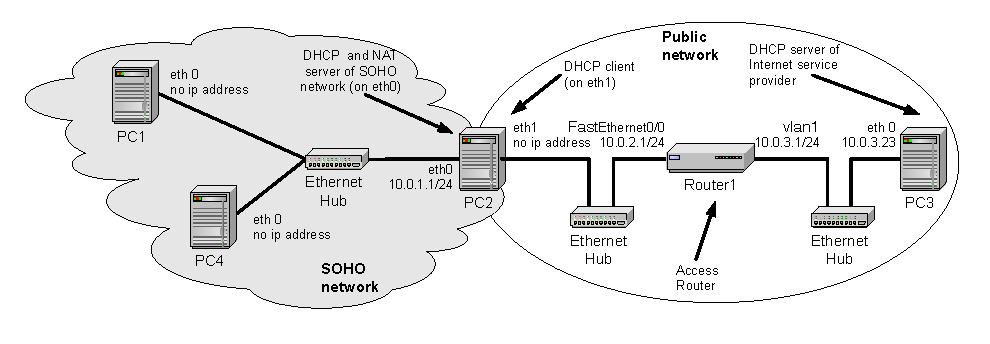
\includegraphics{graphics/lab7-part3-updated.pdf}	
	\caption{Network configuration for Part 3.}
	\label{fig:lab7-part3}
\end{figure}

\subsection{Exercise 3:}
\boxwarning{You will use Wireshark in this exercise. Do not forget to append the binary dump (pcap format) to your lab report}

The network configuration is shown as Figure \ref{fig:lab7-part3}. (The connections of the cables are identical to Figure \ref{fig:lab7-part2}). To reset the configuration of all machines, we recommend rebooting the PCs and the router.

\begin{enumerate}
	\item DHCP Server: PC3 is the DHCP server of the Internet service provider.
		\begin{itemize}
			\item Configure PC3 with IP address 10.0.3.23/24 on interface \iface{eth0} and with default gateway 10.0.3.1.
			\item Configure and start a DHCP server on PC3. On PC3, set up the configuration file so that IP addresses in the range 10.0.2.2-10.0.2.10 are assigned for requests on network 10.0.2.0/24, and addresses in the range 10.0.3.2-10.0.3.10 are assigned for requests on network 10.0.3.0/24.
		\end{itemize}
	\item Router and DHCP relay agent: Router1 is the IP router to which the SOHO network sends its external traffic. Also, Router1 is a DHCP relay agent.
		\begin{itemize}
			\item Configure Router1 with IP addresses 10.0.2.1/24 on interface \iface{FastEthernet0/0} and 10.0.3.1/24 on interface \iface{vlan1}.
			\item The routing table of Router1 should reflect that all traffic to network 10.0.2.0/24 is sent on interface \iface{FastEthernet0/0}, and all other traffic is sent on interface \iface{vlan1}.
			\item Configure Router1 as a DHCP relay agent, so that requests from DHCP client PC2 reach DHCP server PC3.
		\end{itemize}
	\item SOHO Router: PC2 is the SOHO router.
		\begin{itemize}
			\item Set up PC2 so that it is a DHCP client on interface \iface{eth1}.
			\item Set up PC2 as an IP router. That is, IP forwarding must be enabled. The routing table entries must reflect that traffic to network 10.0.1.0/24 must be routed on interface \iface{eth0}, and all other traffic must be sent to Router1 at 10.0.2.1.
			\item Configure PC2 as DHCP server on interface \iface{eth0} for addresses in the range 0.0.1.2 - 10.0.1.10. Execute the following command to start a DHCP server process on PC2:
				\begin{cmdblock}
	PC2% dhcpd eth0
				\end{cmdblock}
			\item Start a NAT server on PC2 and set up a NAT table, which maps packets from the SOHO network with source IP address from network 10.0.1.0/24 to the IP address of interface \iface{eth1}, PC2 obtained through DHCP protocol from PC3. The command for adding a rule that will achieve this is:
				\begin{cmdblock}
	iptables -t nat -A POSTROUTING -j MASQUERADE -o eth1 -s 10.0.1.0/24
				\end{cmdblock}
		\end{itemize}
	\item Hosts in PCs: PC1 and PC4 are hosts in the SOHO network.
		\begin{itemize}
			\item Set up PC1 and PC4 as DHCP clients on interfaces \iface{eth0}.
		\end{itemize}
	\item Collecting the results:
		\begin{itemize}
			\item Display the routing tables from all PCs with \cmd{netstat -rn}, and the IP configuration with \cmd{ifconfig -a}, and save the results.
			\item What are the IP addresses assigned to PC1 and PC4? How are the IP addresses mapped to the public IP address defined on the NAT server PC2?
			\item Display and save the NAT table of PC2.
			\item Start Wireshark on PC1 (\iface{eth0}), PC2 (\iface{eth1}), and PC3 (\iface{eth0}).
			\item Issue a \cmd{ping} command from PC1 to PC3:
				\begin{cmdblock}
	PC1% ping -c 5 10.0.3.23
				\end{cmdblock}
			\item Save the traffic captured by Wireshark on one of the PCs to a file.
		\end{itemize}
\end{enumerate}

\begin{questions}
	\q{3.a}{Include the Wireshark data from the first ICMP Request and ICMP Reply messages.}
	\q{3.b}{Include the routing table and the output of the \cmd{ifconfig} command from all PCs.}
	\q{3.c}{Include the NAT table form PC2.}
\end{questions}

\backmatter

\end{document}
 
